\documentclass[]{book}
\usepackage{lmodern}
\usepackage{amssymb,amsmath}
\usepackage{ifxetex,ifluatex}
\usepackage{fixltx2e} % provides \textsubscript
\ifnum 0\ifxetex 1\fi\ifluatex 1\fi=0 % if pdftex
  \usepackage[T1]{fontenc}
  \usepackage[utf8]{inputenc}
\else % if luatex or xelatex
  \ifxetex
    \usepackage{mathspec}
  \else
    \usepackage{fontspec}
  \fi
  \defaultfontfeatures{Ligatures=TeX,Scale=MatchLowercase}
\fi
% use upquote if available, for straight quotes in verbatim environments
\IfFileExists{upquote.sty}{\usepackage{upquote}}{}
% use microtype if available
\IfFileExists{microtype.sty}{%
\usepackage[]{microtype}
\UseMicrotypeSet[protrusion]{basicmath} % disable protrusion for tt fonts
}{}
\PassOptionsToPackage{hyphens}{url} % url is loaded by hyperref
\usepackage[unicode=true]{hyperref}
\hypersetup{
            pdftitle={Aprendizaje Estadístico},
            pdfauthor={Rubén Fernández Casal (ruben.fcasal@udc.es), Julián Costa (julian.costa@udc.es)},
            pdfborder={0 0 0},
            breaklinks=true}
\urlstyle{same}  % don't use monospace font for urls
\usepackage{natbib}
\bibliographystyle{apalike}
\usepackage{color}
\usepackage{fancyvrb}
\newcommand{\VerbBar}{|}
\newcommand{\VERB}{\Verb[commandchars=\\\{\}]}
\DefineVerbatimEnvironment{Highlighting}{Verbatim}{commandchars=\\\{\}}
% Add ',fontsize=\small' for more characters per line
\usepackage{framed}
\definecolor{shadecolor}{RGB}{248,248,248}
\newenvironment{Shaded}{\begin{snugshade}}{\end{snugshade}}
\newcommand{\KeywordTok}[1]{\textcolor[rgb]{0.13,0.29,0.53}{\textbf{#1}}}
\newcommand{\DataTypeTok}[1]{\textcolor[rgb]{0.13,0.29,0.53}{#1}}
\newcommand{\DecValTok}[1]{\textcolor[rgb]{0.00,0.00,0.81}{#1}}
\newcommand{\BaseNTok}[1]{\textcolor[rgb]{0.00,0.00,0.81}{#1}}
\newcommand{\FloatTok}[1]{\textcolor[rgb]{0.00,0.00,0.81}{#1}}
\newcommand{\ConstantTok}[1]{\textcolor[rgb]{0.00,0.00,0.00}{#1}}
\newcommand{\CharTok}[1]{\textcolor[rgb]{0.31,0.60,0.02}{#1}}
\newcommand{\SpecialCharTok}[1]{\textcolor[rgb]{0.00,0.00,0.00}{#1}}
\newcommand{\StringTok}[1]{\textcolor[rgb]{0.31,0.60,0.02}{#1}}
\newcommand{\VerbatimStringTok}[1]{\textcolor[rgb]{0.31,0.60,0.02}{#1}}
\newcommand{\SpecialStringTok}[1]{\textcolor[rgb]{0.31,0.60,0.02}{#1}}
\newcommand{\ImportTok}[1]{#1}
\newcommand{\CommentTok}[1]{\textcolor[rgb]{0.56,0.35,0.01}{\textit{#1}}}
\newcommand{\DocumentationTok}[1]{\textcolor[rgb]{0.56,0.35,0.01}{\textbf{\textit{#1}}}}
\newcommand{\AnnotationTok}[1]{\textcolor[rgb]{0.56,0.35,0.01}{\textbf{\textit{#1}}}}
\newcommand{\CommentVarTok}[1]{\textcolor[rgb]{0.56,0.35,0.01}{\textbf{\textit{#1}}}}
\newcommand{\OtherTok}[1]{\textcolor[rgb]{0.56,0.35,0.01}{#1}}
\newcommand{\FunctionTok}[1]{\textcolor[rgb]{0.00,0.00,0.00}{#1}}
\newcommand{\VariableTok}[1]{\textcolor[rgb]{0.00,0.00,0.00}{#1}}
\newcommand{\ControlFlowTok}[1]{\textcolor[rgb]{0.13,0.29,0.53}{\textbf{#1}}}
\newcommand{\OperatorTok}[1]{\textcolor[rgb]{0.81,0.36,0.00}{\textbf{#1}}}
\newcommand{\BuiltInTok}[1]{#1}
\newcommand{\ExtensionTok}[1]{#1}
\newcommand{\PreprocessorTok}[1]{\textcolor[rgb]{0.56,0.35,0.01}{\textit{#1}}}
\newcommand{\AttributeTok}[1]{\textcolor[rgb]{0.77,0.63,0.00}{#1}}
\newcommand{\RegionMarkerTok}[1]{#1}
\newcommand{\InformationTok}[1]{\textcolor[rgb]{0.56,0.35,0.01}{\textbf{\textit{#1}}}}
\newcommand{\WarningTok}[1]{\textcolor[rgb]{0.56,0.35,0.01}{\textbf{\textit{#1}}}}
\newcommand{\AlertTok}[1]{\textcolor[rgb]{0.94,0.16,0.16}{#1}}
\newcommand{\ErrorTok}[1]{\textcolor[rgb]{0.64,0.00,0.00}{\textbf{#1}}}
\newcommand{\NormalTok}[1]{#1}
\usepackage{longtable,booktabs}
% Fix footnotes in tables (requires footnote package)
\IfFileExists{footnote.sty}{\usepackage{footnote}\makesavenoteenv{long table}}{}
\usepackage{graphicx,grffile}
\makeatletter
\def\maxwidth{\ifdim\Gin@nat@width>\linewidth\linewidth\else\Gin@nat@width\fi}
\def\maxheight{\ifdim\Gin@nat@height>\textheight\textheight\else\Gin@nat@height\fi}
\makeatother
% Scale images if necessary, so that they will not overflow the page
% margins by default, and it is still possible to overwrite the defaults
% using explicit options in \includegraphics[width, height, ...]{}
\setkeys{Gin}{width=\maxwidth,height=\maxheight,keepaspectratio}
\IfFileExists{parskip.sty}{%
\usepackage{parskip}
}{% else
\setlength{\parindent}{0pt}
\setlength{\parskip}{6pt plus 2pt minus 1pt}
}
\setlength{\emergencystretch}{3em}  % prevent overfull lines
\providecommand{\tightlist}{%
  \setlength{\itemsep}{0pt}\setlength{\parskip}{0pt}}
\setcounter{secnumdepth}{5}
% Redefines (sub)paragraphs to behave more like sections
\ifx\paragraph\undefined\else
\let\oldparagraph\paragraph
\renewcommand{\paragraph}[1]{\oldparagraph{#1}\mbox{}}
\fi
\ifx\subparagraph\undefined\else
\let\oldsubparagraph\subparagraph
\renewcommand{\subparagraph}[1]{\oldsubparagraph{#1}\mbox{}}
\fi

% set default figure placement to htbp
\makeatletter
\def\fps@figure{htbp}
\makeatother

\usepackage{booktabs}
\usepackage{amsthm}
\usepackage[a4paper, top=3.25cm, bottom=2.5cm, left=3cm, right=2.5cm]{geometry}
%\usepackage{fontspec}
%\setmainfont{Arial}
% Espacio después de teorema
% https://tex.stackexchange.com/questions/37797/theorem-environment-line-break-after-label
\newtheoremstyle{break}
  {\topsep}{\topsep}%
  {\itshape}{}%
  {\bfseries}{}%
  {\newline}%
  {}%

\theoremstyle{break}

\ifxetex
  \usepackage{polyglossia}
  \setmainlanguage{spanish}
  % Tabla en lugar de cuadro
  \gappto\captionsspanish{\renewcommand{\tablename}{Tabla}
          \renewcommand{\listtablename}{Índice de tablas}}

\else
  \usepackage[spanish,es-tabla]{babel}
\fi
\makeatletter
\def\thm@space@setup{
  \thm@preskip=8pt plus 2pt minus 4pt
  \thm@postskip=\thm@preskip
}
\makeatother

\title{Aprendizaje Estadístico}
\author{Rubén Fernández Casal
(\href{mailto:ruben.fcasal@udc.es}{\nolinkurl{ruben.fcasal@udc.es}}),
Julián Costa
(\href{mailto:julian.costa@udc.es}{\nolinkurl{julian.costa@udc.es}})}
\date{2020-10-20}

\usepackage{amsthm}
\newtheorem{theorem}{Teorema}[chapter]
\newtheorem{lemma}{Lema}[chapter]
\newtheorem{corollary}{Corolario}[chapter]
\newtheorem{proposition}{Proposición}[chapter]
\newtheorem{conjecture}{Algoritmo}[chapter]
\theoremstyle{definition}
\newtheorem{definition}{Definición}[chapter]
\theoremstyle{definition}
\newtheorem{example}{Ejemplo}[chapter]
\theoremstyle{definition}
\newtheorem{exercise}{Ejercicio}[chapter]
\theoremstyle{remark}
\newtheorem*{remark}{Nota: }
\newtheorem*{solution}{Solución}
\let\BeginKnitrBlock\begin \let\EndKnitrBlock\end
\begin{document}
\maketitle

{
\setcounter{tocdepth}{1}
\tableofcontents
}
\chapter*{Prólogo}\label{pruxf3logo}
\addcontentsline{toc}{chapter}{Prólogo}

Este libro contiene los apuntes de la asignatura de
\href{http://eamo.usc.es/pub/mte/index.php?option=com_content\&view=article\&id=74}{Aprendizaje
Estadístico} del \href{http://eio.usc.es/pub/mte}{Máster en Técnicas
Estadísticas}.

Este libro ha sido escrito en
\href{http://rmarkdown.rstudio.com}{R-Markdown} empleando el paquete
\href{https://bookdown.org/yihui/bookdown/}{\texttt{bookdown}} y está
disponible en el repositorio Github:
\href{https://github.com/rubenfcasal/aprendizaje_estadistico}{rubenfcasal/aprendizaje\_estadistico}.
Se puede acceder a la versión en línea a través del siguiente enlace:

\url{https://rubenfcasal.github.io/aprendizaje_estadistico}.

donde puede descargarse en formato
\href{https://rubenfcasal.github.io/aprendizaje_estadistico/aprendizaje_estadistico.pdf}{pdf}.

Para ejecutar los ejemplos mostrados en el libro sería necesario tener
instalados los siguientes paquetes:
\href{https://CRAN.R-project.org/package=caret}{\texttt{caret}},
\href{https://CRAN.R-project.org/package=rattle}{\texttt{rattle}},
\href{https://CRAN.R-project.org/package=car}{\texttt{car}},
\href{https://CRAN.R-project.org/package=leaps}{\texttt{leaps}},
\href{https://CRAN.R-project.org/package=MASS}{\texttt{MASS}},
\href{https://CRAN.R-project.org/package=RcmdrMisc}{\texttt{RcmdrMisc}},
\href{https://CRAN.R-project.org/package=lmtest}{\texttt{lmtest}},
\href{https://CRAN.R-project.org/package=glmnet}{\texttt{glmnet}},
\href{https://CRAN.R-project.org/package=mgcv}{\texttt{mgcv}},
\href{https://CRAN.R-project.org/package=AppliedPredictiveModeling}{\texttt{AppliedPredictiveModeling}},
\href{https://CRAN.R-project.org/package=ISLR}{\texttt{ISLR}}. Por
ejemplo mediante los siguientes comandos:

\begin{Shaded}
\begin{Highlighting}[]
\NormalTok{pkgs <-}\StringTok{ }\KeywordTok{c}\NormalTok{(}\StringTok{"caret"}\NormalTok{, }\StringTok{"rattle"}\NormalTok{, }\StringTok{"car"}\NormalTok{, }\StringTok{"leaps"}\NormalTok{, }\StringTok{"MASS"}\NormalTok{, }\StringTok{"RcmdrMisc"}\NormalTok{, }
          \StringTok{"lmtest"}\NormalTok{, }\StringTok{"glmnet"}\NormalTok{, }\StringTok{"mgcv"}\NormalTok{, }
          \StringTok{"AppliedPredictiveModeling"}\NormalTok{, }\StringTok{"ISLR"}\NormalTok{)}

\KeywordTok{install.packages}\NormalTok{(}\KeywordTok{setdiff}\NormalTok{(pkgs, }\KeywordTok{installed.packages}\NormalTok{()[,}\StringTok{"Package"}\NormalTok{]), }\DataTypeTok{dependencies =} \OtherTok{TRUE}\NormalTok{)}
\CommentTok{# Si aparecen errores (normalmente debidos a incompatibilidades con versiones ya instaladas), }
\CommentTok{# probar a ejecutar en lugar de lo anterior:}
\CommentTok{# install.packages(pkgs, dependencies=TRUE) # Instala todos...}
\end{Highlighting}
\end{Shaded}

Para generar el libro (compilar) serán necesarios paquetes adicionales,
para lo que se recomendaría consultar el libro de
\href{https://rubenfcasal.github.io/bookdown_intro}{``Escritura de
libros con bookdown''} en castellano.


\includegraphics[width=1.22in]{images/by-nc-nd-88x31}

Este obra está bajo una licencia de
\href{https://creativecommons.org/licenses/by-nc-nd/4.0/deed.es_ES}{Creative
Commons Reconocimiento-NoComercial-SinObraDerivada 4.0 Internacional}
(esperamos poder liberarlo bajo una licencia menos restrictiva más
adelante\ldots{}).

\chapter{Introducción al Aprendizaje Estadístico}\label{intro-AE}

La denominada \emph{Ciencia de Datos} (Data Science; también denominada
\emph{Science of Learning}) se ha vuelto muy popular hoy en día. Se
trata de un campo multidisciplicar, con importantes aportaciones
estadísticas e informáticas, dentro del que se incluirían disciplinas
como \emph{Minería de Datos} (Data Mining), \emph{Aprendizaje
Automático} (Machine Learning), \emph{Aprendizaje Profundo} (Deep
Learning), \emph{Modelado Predictivo} (Predictive Modeling),
\emph{Extracción de Conocimiento} (Knowlegde Discovery) y también el
\emph{Aprendizaje Estadístico} (Statistical Learning).

Podríamos definir la Ciencia de Datos como el conjunto de conocimientos
y herramientas utilizados en las distintas etapas del análisis de datos
(ver Figura \ref{fig:esquema}). Otras definiciones podrían ser:

\begin{itemize}
\item
  El arte y la ciencia del análisis inteligente de los datos.
\item
  El conjunto de herramientas para entender y modelizar conjuntos
  (complejos) de datos.
\item
  El proceso de descubrir patrones y obtener conocimiento a partir de
  grandes conjuntos de datos (\emph{Big Data}).
\end{itemize}

Aunque esta ciencia incluiría también la gestión (sin olvidarnos del
proceso de obtención) y la manipulación de los datos.

\begin{figure}[!htb]

{\centering 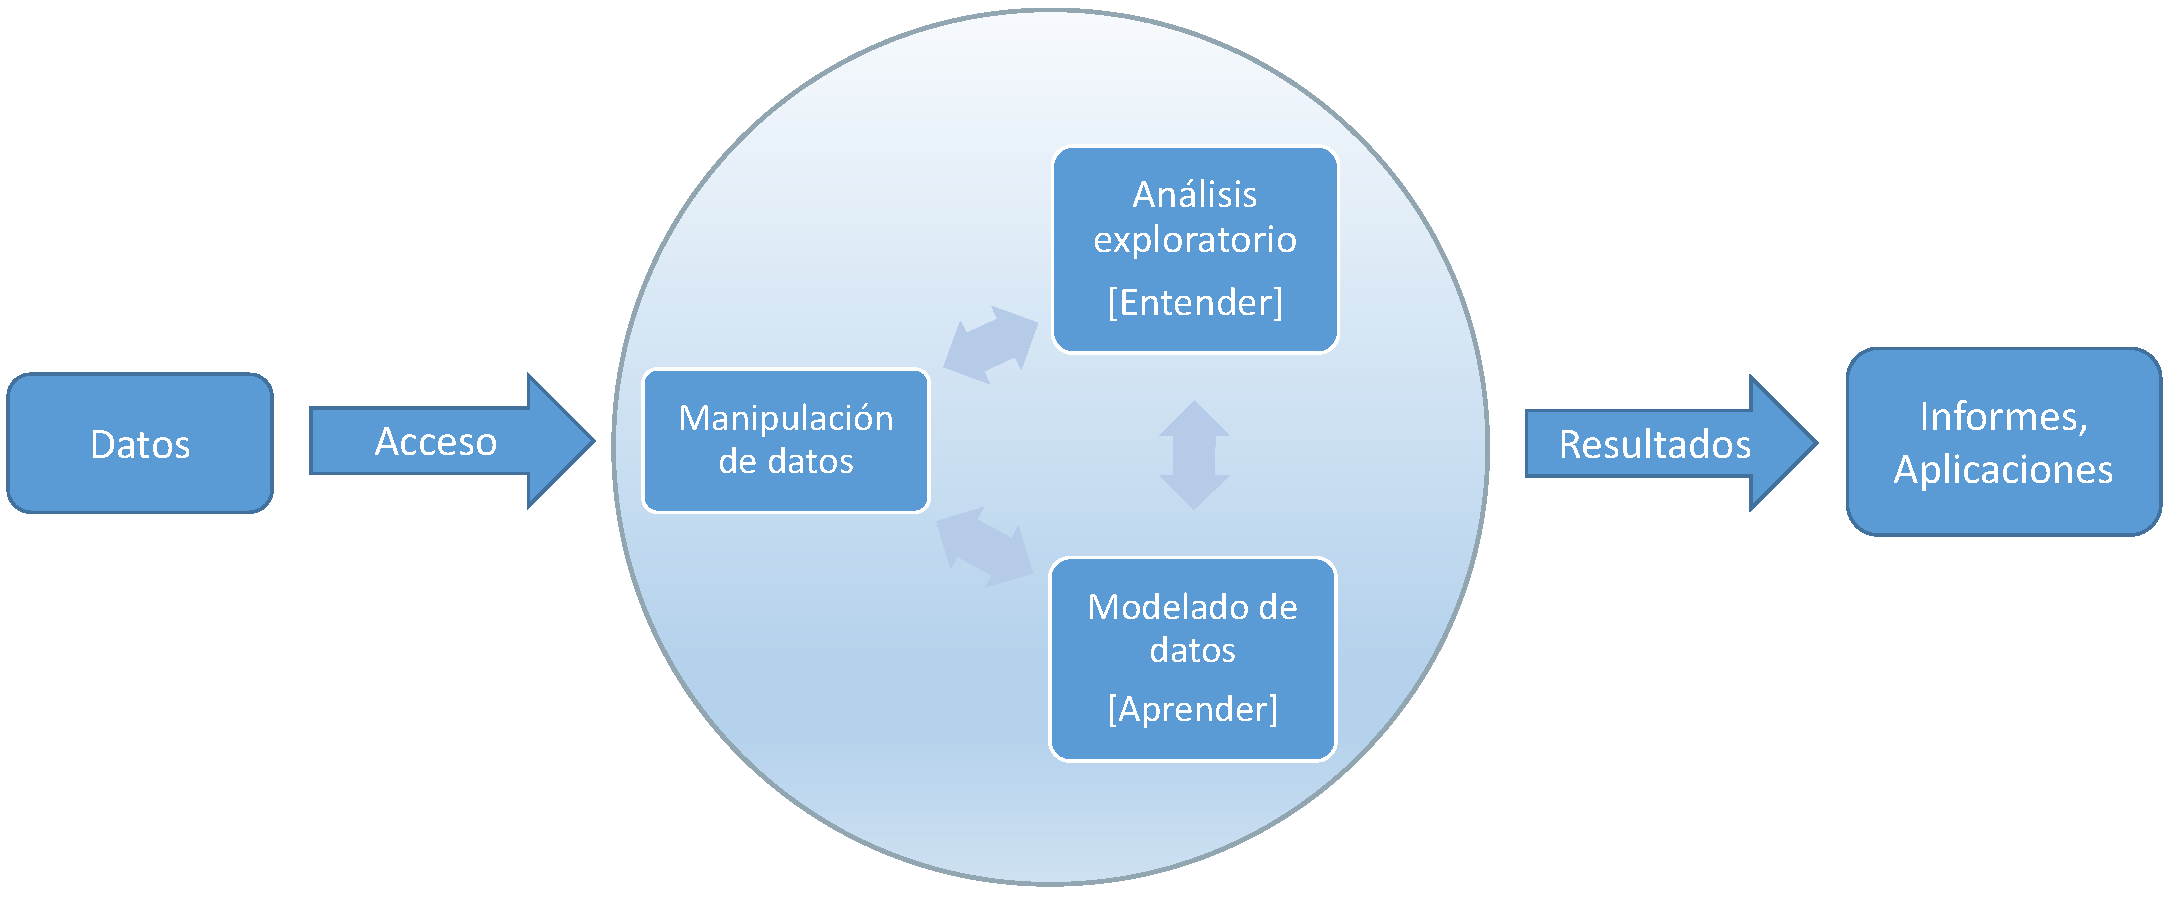
\includegraphics[width=0.8\linewidth]{images/esquema2} 

}

\caption{Etapas del proceso}\label{fig:esquema}
\end{figure}

Una de estas etapas (que están interrelacionadas) es la construcción de
modelos a partir de los datos para aprender y predecir. Podríamos decir
que el Aprendizaje Estadístico (AE) se encarga de este problema desde el
punto de vista estadístico.

En Estadística se consideran modelos estocásticos (con componente
aleatoria), para tratar de tener en cuenta la incertidumbre debida a que
no se disponga de toda la información (sobre las variables que influyen
en el fenómeno de interés).

\begin{quote}
``Nothing in Nature is random\ldots{} a thing appears random only
through the incompleteness of our knowledge.''

--- Spinoza, Baruch (Ethics, 1677)
\end{quote}

\begin{quote}
``To my mind, although Spinoza lived and thought long before Darwin,
Freud, Einstein, and the startling implications of quantum theory, he
had a vision of truth beyond what is normally granted to human beings.''

--- Shirley, Samuel (Complete Works, 2002). Traductor de la obra
completa de Spinoza al inglés.
\end{quote}

La Inferencia Estadística proporciona herramientas para ajustar este
tipo de modelos a los datos observados (seleccionar un modelo adecuado,
estimar sus parámetros y contrastar su validez). Sin embargo, en la
aproximación estadística clásica como primer objetivo se trata de
explicar por completo lo que ocurre en la población y suponiendo que
esto se puede hacer con modelos tratables analíticamente, emplear
resultados teóricos (típicamente resultados asintóticos) para realizar
inferencias (entre ellas la predicción). Los avances en computación han
permitido el uso de modelos estadísticos más avanzados, principalmente
métodos no paramétricos, muchos de los cuales no pueden ser tratados
analíticamente (por lo menos no por completo o no inicialmente), este es
el campo de la Estadística Computacional\footnote{Lauro (1996) definió
  la Estadística Computacional como la disciplina que tiene como
  objetivo ``diseñar algoritmos para implementar métodos estadísticos en
  computadoras, incluidos los impensables antes de la era de las
  computadoras (por ejemplo, bootstrap, simulación), así como hacer
  frente a problemas analíticamente intratables''.}. Desde este punto de
vista, el AE se enmarcaría dentro del campo de la Estadística
Computacional.

Cuando pensamos en AE pensamos en:

\begin{itemize}
\item
  Flexibilidad (hay menos suposiciones sobre los datos).
\item
  Procesamiento automático de datos.
\item
  Big Data (en el sentido amplio, donde ``big'' puede hacer referencia a
  datos complejos).
\item
  Predicción.
\end{itemize}

Por el contrario, muchos de los métodos del AE no se preocupan (o se
preocupan poco) por:

\begin{itemize}
\item
  Reproducibilidad.
\item
  Cuantificación de la incertidumbre (en términos de probabilidad).
\item
  Inferencia.
\end{itemize}

La idea es ``dejar hablar a los datos'' y no ``encorsetarlos'' a priori,
dándoles mayor peso que a los modelos. Sin embargo, esta aproximación
puede presentar diversos inconvenientes:

\begin{itemize}
\item
  Algunos métodos son poco interpretables (se sacrifica la
  interpretabilidad por la precisión de las predicciones).
\item
  Pueden aparecer problemas de sobreajuste (\emph{overfitting}; en los
  métodos estadísticos clásicos es más habitual que aparezcan problemas
  de infraajuste, \emph{underfitting}).
\item
  Pueden presentar más problemas al extrapolar o interpolar (en
  comparación con los métodos clásicos).
\end{itemize}

\section{Aprendizaje Estadístico vs.~Aprendizaje
Automático}\label{aprendizaje-estaduxedstico-vs.aprendizaje-automuxe1tico}

El término \emph{Machine Learning} (ML; Aprendizaje Automático) se
utiliza en el campo de la \emph{Intelingencia Artificial} desde 1959
para hacer referencia, fundamentalmente, a algoritmos de predicción
(inicialmente para reconocimiento de patrones). Muchas de las
herramientas que utilizan provienen del campo de la Estadística y, en
cualquier caso, la Estadística (y por tanto las Matemáticas) es la base
de todos estos enfoques para analizar datos (y no conviene perder la
base formal). Por este motivo desde la Estadística Computacional se
introdujo el término \emph{Statistical Learning} (Aprendizaje
Estadístico) para hacer referencia a este tipo de herramientas, pero
desde el punto de vista estadístico (teniendo en cuenta la incertidumbre
debida a no disponer de toda la información).

Tradicionalmente ML no se preocupa del origen de los datos e incluso es
habitual que se considere que un conjunto enorme de datos es equivalente
a disponer de toda la información (i.e.~a la población).

\begin{quote}
``The sheer volume of data would obviate the need of theory and even
scientific method''

--- Chris Anderson, físico y periodista, 2008
\end{quote}

Por el contrario en el caso del AE se trata de comprender, si es
posible, el proceso subyacente del que provienen los datos y si estos
son representativos de la población de interés (i.e.~si tienen algún
tipo de sesgo). No obstante, en este libro se considerará en general
ambos términos como sinónimos.

ML/AE hacen un importante uso de la programación matemática, ya que
muchos de sus problemas se plantean en términos de la optimización de
funciones bajo restricciones. Recíprocamente, en optimización también se
utilizan algoritmos de ML/AE.

\subsection{Machine Learning vs.~Data
Mining}\label{machine-learning-vs.data-mining}

Mucha gente utiliza indistintamente los nombres ML y \emph{Data Mining}
(DM). Sin embargo, aunque tienen mucho solapamiento, lo cierto es que
hacen referencia a conceptos ligeramente distintos.

ML es un conjunto de algoritmos principalmente dedicados a hacer
predicciones y que son esencialmente automáticos minimizando la
intervención humana.

DM intenta \emph{entender} conjuntos de datos (en el sentido de
encontrar sus patrones), requiere de una intervención humana activa (al
igual que la Inferencia Estadística tradicional), pero utiliza entre
otras las técnicas automáticas de ML. Por tanto podríamos pensar que es
más parecido al AE.

\subsection{Las dos culturas (Breiman,
2001)}\label{las-dos-culturas-breiman-2001}

Breiman diferencia dos objetivos en el análisis de datos, que él llama
\emph{información} (en el sentido de \emph{inferencia}) y
\emph{predicción}. Cada uno de estos objetivos da lugar a una cultura:

\begin{itemize}
\item
  \emph{Modelización de datos}: desarrollo de modelos (estocásticos) que
  permitan ajustar los datos y hacer inferencia. Es el trabajo habitual
  de los estadísticos académicos.
\item
  \emph{Modelización algorítmica} (en el sentido de predictiva): esta
  cultura no está interesada en los mecanismos que generan los datos,
  sólo en los algoritmos de predicción. Es el trabajo habitual de muchos
  estadísticos industriales y de muchos ingenieros informáticos. El ML
  es el núcleo de esta cultura que pone todo el énfasis en la precisión
  predictiva (así, un importante elemento dinamizador son las
  competiciones entre algoritmos predictivos, al estilo del
  \href{https://en.wikipedia.org/wiki/Netflix_Prize}{Netflix
  Challenge}).
\end{itemize}

\subsection{Machine Learning vs.~Estadística (Dunson,
2018)}\label{machine-learning-vs.estaduxedstica-dunson-2018}

\begin{itemize}
\item
  ``Machine learning: The main publication outlets tend to be
  peer-reviewed conference proceedings and the style of research is very
  fast paced, trendy, and driven by performance metrics in prediction
  and related tasks''.
\item
  ``Statistical community: The main publication outlets are
  peer-reviewed journals, most of which have a long drawn out review
  process, and the style of research tends to be careful, slower paced,
  intellectual as opposed to primarily performance driven, emphasizing
  theoretical support (e.g., through asymptotic properties),
  under-stated, and conservative''.
\item
  ``\emph{Big data} in ML typically means that the number of examples
  (i.e.~sample size) is very large''.
\item
  ``In statistics (\ldots{}) it has become common to collect high
  dimensional, complex and intricately structured data. Often the
  dimensionality of the data vastly exceeds the available sample size,
  and the fundamental challenge of the statistical analysis is obtaining
  new insights from these huge data, while maintaining
  reproducibility/replicability and reliability of the results''.
\end{itemize}

\section{Métodos de Aprendizaje
Estadístico}\label{muxe9todos-de-aprendizaje-estaduxedstico}

Dentro de los problemas que aborda el Aprendizaje Estadístico se suelen
diferenciar dos grandes bloques: el aprendizaje no supervisado y el
supervisado. El \emph{aprendizaje no supervisado} comprende los métodos
exploratorios, es decir, aquellos en los que no hay una variable
respuesta (al menos no de forma explícita). El principal objetivo de
estos métodos es entender las relaciones entre los datos y su
estructura, y pueden clasificarse en las siguientes categorías:

\begin{itemize}
\item
  Análisis descriptivo.
\item
  Métodos de reducción de la dimensión (análisis de componentes
  principales, análisis factorial\ldots{}).
\item
  Clúster.
\item
  Detección de datos atípicos.
\end{itemize}

El \emph{aprendizaje supervisado} engloba los métodos predictivos, en
los que una de las variables está definida como variable respuesta. Su
principal objetivo es la construcción de modelos que posteriormente se
utilizarán, sobre todo, para hacer predicciones. Dependiendo del tipo de
variable respuesta se diferencia entre:

\begin{itemize}
\item
  Clasificación: respuesta categórica (también se emplea la denominación
  de variable cualitativa, discreta o factor).
\item
  Regresión: respuesta numérica (cuantitativa).
\end{itemize}

En este libro nos centraremos únicamente en el campo del aprendizaje
supervisado y combinaremos la terminología propia de la Estadística con
la empleada en AE (por ejemplo, en Estadística es habitual considerar un
problema de clasificación como un caso particular de regresión).

\subsection{Notación y terminología}\label{notacion}

Denotaremos por \(\mathbf{X}=(X_1, X_2, \ldots, X_p)\) al vector formado
por las variables predictoras (variables explicativas o variables
independientes; también \emph{inputs} o \emph{features} en la
terminología de ML), cada una de las cuales podría ser tanto numérica
como categórica\footnote{Aunque hay que tener en cuenta que algunos
  métodos están diseñados para predictores numéricos, otros para
  categóricos y algunos para ambos tipos.}. En general (ver comentarios
más adelante), emplearemos \(Y\left(\mathbf{X} \right)\) para referirnos
a la variable objetivo (variable respuesta o variable dependiente;
también \emph{output} en la terminología de ML), que como ya se comentó
puede ser una variable numérica (regresión) o categórica
(clasificación).

Supondremos que el objetivo principal es, a partir de una muestra:
\[\left\{ \left( x_{1i}, \ldots, x_{pi}, y_{i} \right)  : i = 1, \ldots, n \right\},\]
obtener (futuras) predicciones \(\hat Y\left(\mathbf{x} \right)\) de la
respuesta para
\(\mathbf{X}=\mathbf{x}=\left(x_{1}, \ldots, x_{p}\right)\).

En regresión consideraremos como base el siguiente modelo general
(podría ser después de una transformación de la respuesta):

\begin{equation} 
  Y(\mathbf{X})=m(\mathbf{X})+\varepsilon,
  \label{eq:modelogeneral}
\end{equation}

donde
\(m(\mathbf{x}) = E\left( \left. Y\right\vert_{\mathbf{X}=\mathbf{x}} \right)\)
es la media condicional, denominada función de regresión (o tendencia),
y \(\varepsilon\) es un error aleatorio de media cero y varianza
\(\sigma^2\), independiente de \(\mathbf{X}\). Este modelo puede
generalizarse de diversas formas, por ejemplo, asumiendo que la
distribución del error depende de \(X\) (considerando
\(\varepsilon(\mathbf{X})\) en lugar de \(\varepsilon\)) podríamos
incluir dependencia y heterocedasticidad. En estos casos normalmente se
supone que lo hace únicamente a través de la varianza (error
heterocedástico independiente), denotando por
\(\sigma^2(\mathbf{x}) = Var\left( \left. Y\right\vert_{\mathbf{X}=\mathbf{x}} \right)\)
la varianza condicional\footnote{Por ejemplo considerando en el modelo
  base \(\sigma(\mathbf{X})\varepsilon\) como termino de error y
  suponiendo adicionalmente que \(\varepsilon\) tiene varianza uno.}.

Como ya se comentó se podría considerar clasificación como un caso
particular, por ejemplo definiendo \(Y\left(\mathbf{X} \right)\) de
forma que tome los valores \(1, 2, \ldots, K\), etiquetas que
identifican las \(K\) posibles categorías (también se habla de
modalidades, niveles, clases o grupos). Sin embargo, muchos métodos de
clasificación emplean variables auxiliares (variables \emph{dummy}),
indicadoras de las distintas categorías, y emplearemos la notación
anterior para referirnos a estas variables (también denominadas
variables \emph{target}). En cuyo caso, denotaremos por
\(G \left(\mathbf{X} \right)\) la respuesta categórica (la clase
verdadera; \(g_i\), \(i =1, \ldots, n\), serían los valores observados)
y por \(\hat G \left(\mathbf{X} \right)\) el predictor.

Por ejemplo, en el caso de dos categorías, se suele definir \(Y\) de
forma que toma el valor 1 en la categoría de interés (también denominada
\emph{éxito} o \emph{resultado positivo}) y 0 en caso contrario
(\emph{fracaso} o \emph{resultado negativo})\footnote{Otra alternativa
  sería emplear 1 y -1, algo que simplifica las expresiones de algunos
  métodos.}. Además, en este caso, los modelos típicamente devuelven
estimaciones de la probabilidad de la clase de interés en lugar de
predecir directamente la clase, por lo que se empleará \(\hat p\) en
lugar de \(\hat Y\). A partir de esa estimación se obtiene una
predicción de la categoría. Normalmente se predice la clase más
probable, i.e. ``éxito'' si \(\hat p(\mathbf{x}) > c = 0.5\) y
``fracaso'' en caso contrario (con probabilidad estimada
\(1 - \hat p(\mathbf{x})\)).

Resulta claro que el modelo base general \eqref{eq:modelogeneral} puede no
ser adecuado para modelar variables indicadoras (o probabilidades).
Muchos de los métodos de AE emplean \eqref{eq:modelogeneral} para una
variable auxiliar numérica (denominada puntuación o \emph{score}) que se
transforma a escala de probabilidades mediante la función logística
(denominada función sigmoidal, \emph{sigmoid function}, en ML)\footnote{De
  especial interés en regresión logística y en redes neuronales
  artificiales.}: \[p(s) = \frac{1}{1 + e^{-s}},\] cuya inversa es la
\emph{función logit}:
\[\operatorname{logit}(p)=\log\left( \frac{p}{1-p} \right).\]

Lo anterior se puede generalizar para el caso de múltiples categorías,
considerando variables indicadoras de cada categoría
\(Y_1, \ldots, Y_K\) (es lo que se conoce como la estrategia de ``uno
contra todos''). En este caso típicamente:
\[\hat G \left(\mathbf{x} \right) = \underset{k}{\operatorname{argmax}} \left\{ \hat p_k(\mathbf{x}) : k = 1, 2, \ldots, K \right\}.\]

\subsection{Métodos (de aprendizaje supervisado) y paquetes de
R}\label{metodos-pkgs}

Hay una gran cantidad de métodos de aprendizaje supervisado
implementados en centenares de paquetes de \texttt{R} (ver por ejemplo
\href{https://cran.r-project.org/web/views/MachineLearning.html}{CRAN
Task View: Machine Learning \& Statistical Learning}). A continuación se
muestran los principales métodos y algunos de los paquetes de R que los
implementan (muchos son válidos para regresión y clasificación, como por
ejemplo los basados en árboles, aunque aquí aparecen en su aplicación
habitual).

Métodos de Clasificación:

\begin{itemize}
\item
  Análisis discriminante (lineal, cuadrático), Regresión logística,
  multinomial\ldots{}: \texttt{stats}, \texttt{MASS}\ldots{}
\item
  Árboles de decisión, \emph{bagging}, \emph{random forest},
  \emph{boosting}: \texttt{rpart}, \texttt{party}, \texttt{C50},
  \texttt{Cubist}, \texttt{randomForest}, \texttt{adabag},
  \texttt{xgboost}\ldots{}
\item
  \emph{Support vector machines} (SVM): \texttt{kernlab},
  \texttt{e1071}\ldots{}
\end{itemize}

Métodos de regresión:

\begin{itemize}
\item
  Modelos lineales:

  \begin{itemize}
  \item
    Regresión lineal: \texttt{lm()}, \texttt{lme()},
    \texttt{biglm}\ldots{}
  \item
    Regresión lineal robusta: \texttt{MASS::rlm()}\ldots{}
  \item
    Métodos de regularización (Ridge regression, Lasso):
    \texttt{glmnet}, \texttt{elasticnet}\ldots{}
  \end{itemize}
\item
  Modelos lineales generalizados: \texttt{glm()}, \texttt{bigglm}, ..
\item
  Modelos paramétricos no lineales: \texttt{nls()},
  \texttt{nlme}\ldots{}
\item
  Regresión local (vecinos más próximos y métodos de suavizado):
  \texttt{kknn}, \texttt{loess()}, \texttt{KernSmooth}, \texttt{sm},
  \texttt{np}\ldots{}
\item
  Modelos aditivos generalizados (GAM): \texttt{mgcv},
  \texttt{gam}\ldots{}
\item
  Redes neuronales: \texttt{nnet}\ldots{}
\end{itemize}

También existen paquetes de \texttt{R} que permiten utilizar plataformas
de ML externas, como por ejemplo
\href{https://github.com/h2oai/h2o-3/tree/master/h2o-r}{\texttt{h2o}} o
\href{https://CRAN.R-project.org/package=RWeka}{\texttt{RWeka}}.

Como todos estos paquetes emplean opciones, estructuras y convenciones
sintácticas diferentes, se han desarrollado paquetes que proporcionan
interfaces unificadas a muchas de estas implementaciones. Entre ellos
podríamos citar
\href{https://topepo.github.io/caret}{\texttt{caret}},\href{https://mlr3.mlr-org.com}{\texttt{mlr3}}
y \href{https://www.tidymodels.org}{\texttt{tidymodels}}. En la Sección
\ref{caret} se incluye una breve introducción al paquete
\href{https://topepo.github.io/caret}{\texttt{caret}} que será empleado
en diversas ocasiones a lo largo del presente libro.

Adicionalmente hay paquetes de R que disponen de entornos gráficos que
permiten emplear estos métodos evitando el uso de comandos. Entre ellos
estarían R-Commander con el plugin FactoMineR (\texttt{Rcmdr},
\texttt{RcmdrPlugin.FactoMineR}) y
\href{https://rattle.togaware.com}{\texttt{rattle}}.

\section{Construcción y evaluación de los modelos}\label{const-eval}

En Inferencia Estadística clásica el procedimiento habitual es emplear
toda la información disponible para construir un modelo válido (que
refleje de la forma más fiel posible lo que ocurre en la población) y
asumiendo que el modelo es el verdadero (lo que en general sería falso)
utilizar métodos de inferencia para evaluar su precisión. Por ejemplo,
en el caso de regresión lineal múltiple, el coeficiente de determinación
ajustado sería una medida del la precisión del modelo para predecir
nuevas observaciones (no se debería emplear el coeficiente de
determinación sin ajustar; aunque, en cualquier caso, su validez
dependería de la de las suposiciones estructurales del modelo).

Alternativamente, en Estadística Computacional es habitual emplear
técnicas de remuestreo para evaluar la precisión (entrenando también el
modelo con todos los datos disponibles), principalmente validación
cruzada (leave-one-out, k-fold), jackniffe o bootstrap.

Por otra parte, como ya se comentó, algunos de los modelos empleados en
AE son muy flexibles (están hiperparametrizados) y pueden aparecer
problemas si se permite que se ajusten demasiado bien a las
observaciones (podrían llegar a interpolar los datos). En estos casos
habrá que controlar el procedimiento de aprendizaje, típicamente a
traves de parámetros relacionados con la complejidad del modelo (ver
sección siguiente).

En AE se distingue entre parámetros estructurales, los que van a ser
estimados al ajustar el modelo a los datos (en el entrenamiento), e
hiperparámetros (\emph{tuning parameters} o parámetros de ajuste), que
imponen restricciones al aprendizaje del modelo (por ejemplo
determinando el número de parámetros estructurales). Si los
hiperparámetros seleccionados producen un modelo demasiado complejo
aparecerán problemas de sobreajuste (\emph{overfitting}) y en caso
contrario de infraajuste (\emph{undefitting}).

Hay que tener en cuenta también que al aumentar la complejidad disminuye
la interpretabilidad de los modelos. Se trataría entonces de conseguir
buenas predicciones (habrá que evaluar la capacidad predictiva) con el
modelo más sencillo posible.

\subsection{Equilibrio entre sesgo y varianza: infraajuste y
sobreajuste}\label{bias-variance}

La idea es que queremos aprender más allá de los datos empleados en el
entrenamiento (en Estadística diríamos que queremos hacer inferencia
sobre nuevas observaciones). Como ya se comentó, en AE hay que tener
especial cuidado con el sobreajuste. Este problema ocurre cuando el
modelo se ajusta demasiado bien a los datos de entrenamiento pero falla
cuando se utiliza en un nuevo conjunto de datos (nunca antes visto).

Como ejemplo ilustrativo emplearemos regresión polinómica, considerando
el grado del polinomio como un hiperparámetro que determina la
complejidad del modelo. En primer lugar simulamos una muestra y
ajustamos modelos polinómicos con distintos grados de complejidad.

\begin{Shaded}
\begin{Highlighting}[]
\CommentTok{# Simulación datos}
\NormalTok{n <-}\StringTok{ }\DecValTok{30}
\NormalTok{x <-}\StringTok{ }\KeywordTok{seq}\NormalTok{(}\DecValTok{0}\NormalTok{, }\DecValTok{1}\NormalTok{, }\DataTypeTok{length =}\NormalTok{ n)}
\NormalTok{mu <-}\StringTok{ }\DecValTok{2} \OperatorTok{+}\StringTok{ }\DecValTok{4}\OperatorTok{*}\NormalTok{(}\DecValTok{5}\OperatorTok{*}\NormalTok{x }\OperatorTok{-}\StringTok{ }\DecValTok{1}\NormalTok{)}\OperatorTok{*}\NormalTok{(}\DecValTok{4}\OperatorTok{*}\NormalTok{x }\OperatorTok{-}\StringTok{ }\DecValTok{2}\NormalTok{)}\OperatorTok{*}\NormalTok{(x }\OperatorTok{-}\StringTok{ }\FloatTok{0.8}\NormalTok{)}\OperatorTok{^}\DecValTok{2} \CommentTok{# grado 4}
\NormalTok{sd <-}\StringTok{ }\FloatTok{0.5}
\KeywordTok{set.seed}\NormalTok{(}\DecValTok{1}\NormalTok{)}
\NormalTok{y <-}\StringTok{ }\NormalTok{mu }\OperatorTok{+}\StringTok{ }\KeywordTok{rnorm}\NormalTok{(n, }\DecValTok{0}\NormalTok{, sd)}
\KeywordTok{plot}\NormalTok{(x, y) }
\KeywordTok{lines}\NormalTok{(x, mu, }\DataTypeTok{lwd =} \DecValTok{2}\NormalTok{)}
\CommentTok{# Ajuste de los modelos}
\NormalTok{fit1 <-}\StringTok{ }\KeywordTok{lm}\NormalTok{(y }\OperatorTok{~}\StringTok{ }\NormalTok{x)}
\KeywordTok{lines}\NormalTok{(x, }\KeywordTok{fitted}\NormalTok{(fit1))}
\NormalTok{fit2 <-}\StringTok{ }\KeywordTok{lm}\NormalTok{(y }\OperatorTok{~}\StringTok{ }\KeywordTok{poly}\NormalTok{(x, }\DecValTok{4}\NormalTok{))}
\KeywordTok{lines}\NormalTok{(x, }\KeywordTok{fitted}\NormalTok{(fit2), }\DataTypeTok{lty =} \DecValTok{2}\NormalTok{)}
\NormalTok{fit3 <-}\StringTok{ }\KeywordTok{lm}\NormalTok{(y }\OperatorTok{~}\StringTok{ }\KeywordTok{poly}\NormalTok{(x, }\DecValTok{20}\NormalTok{)) }
\CommentTok{# NOTA: poly(x, degree, raw = FALSE) tiene un problema de desbordamiento si degree > 25}
\KeywordTok{lines}\NormalTok{(x, }\KeywordTok{fitted}\NormalTok{(fit3), }\DataTypeTok{lty =} \DecValTok{3}\NormalTok{)}
\KeywordTok{legend}\NormalTok{(}\StringTok{"topright"}\NormalTok{, }\DataTypeTok{legend =} \KeywordTok{c}\NormalTok{(}\StringTok{"Verdadero"}\NormalTok{, }\StringTok{"Ajuste con grado 1"}\NormalTok{, }
                              \StringTok{"Ajuste con grado 4"}\NormalTok{, }\StringTok{"Ajuste con grado 20"}\NormalTok{), }
       \DataTypeTok{lty =} \KeywordTok{c}\NormalTok{(}\DecValTok{1}\NormalTok{, }\DecValTok{1}\NormalTok{, }\DecValTok{2}\NormalTok{, }\DecValTok{3}\NormalTok{), }\DataTypeTok{lwd =} \KeywordTok{c}\NormalTok{(}\DecValTok{2}\NormalTok{, }\DecValTok{1}\NormalTok{, }\DecValTok{1}\NormalTok{, }\DecValTok{1}\NormalTok{))}
\end{Highlighting}
\end{Shaded}

\begin{figure}[!htb]

{\centering 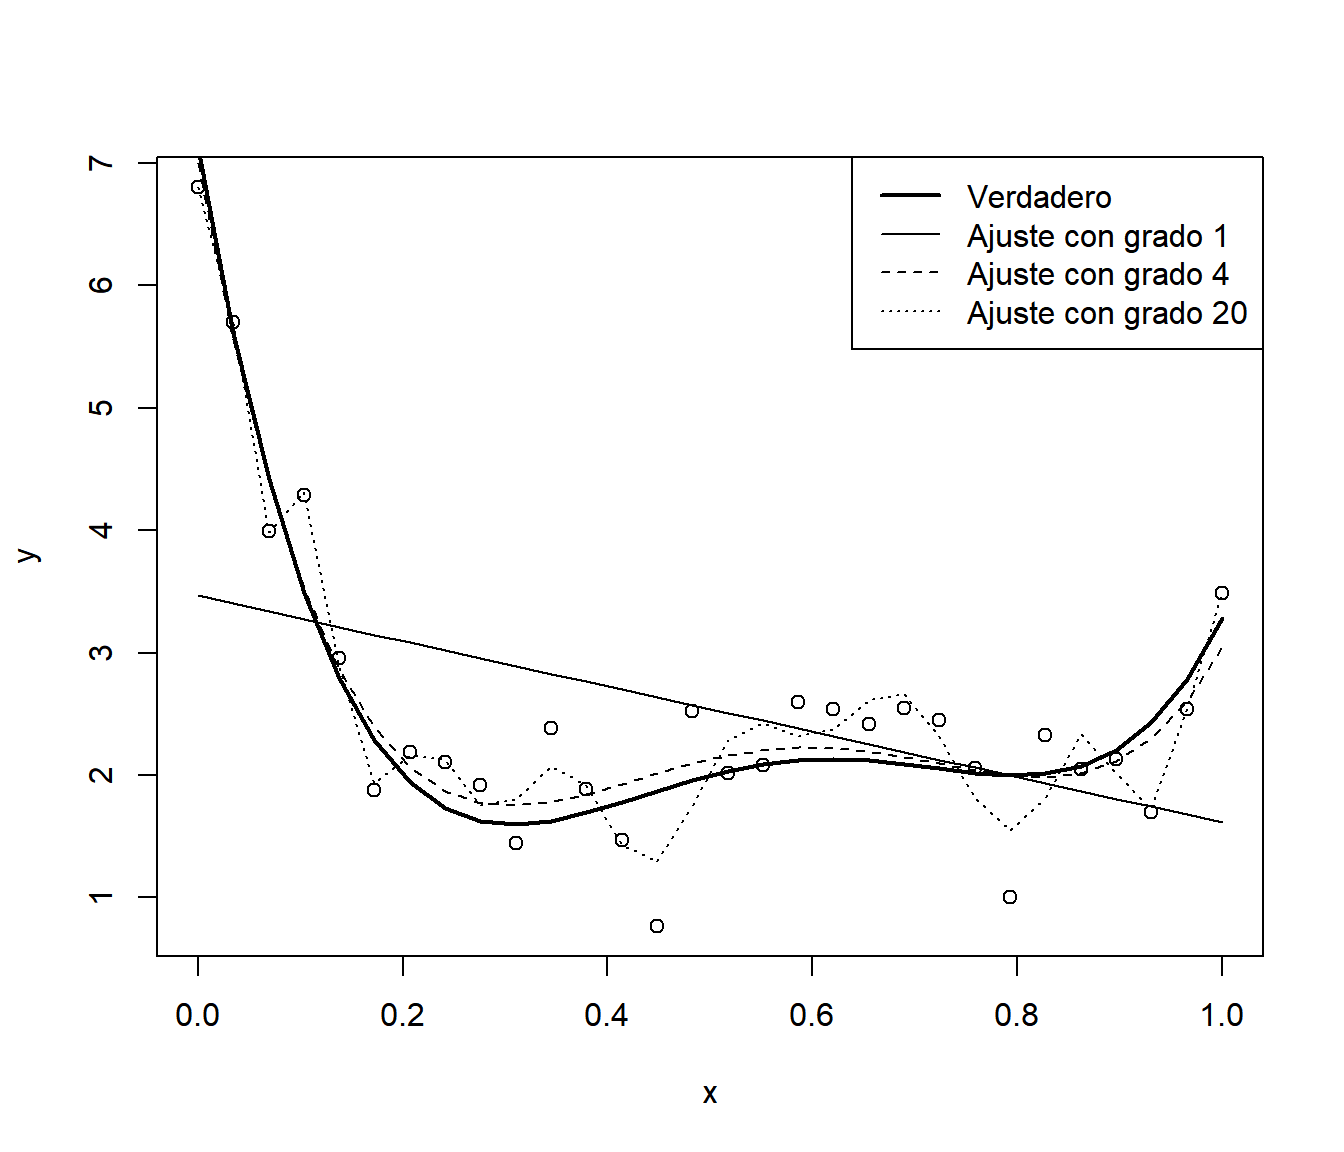
\includegraphics[width=0.8\linewidth]{01-introduccion_files/figure-latex/polyfit-1} 

}

\caption{Muestra (simulada) y ajustes polinómicos con distinta complejidad.}\label{fig:polyfit}
\end{figure}

Como se observa en la Figura \ref{fig:polyfit} al aumentar la
complejidad del modelo se consigue un mejor ajuste a los datos
observados (empleados en el entrenamiento), a costa de un incremento en
la variabilidad de las predicciones, lo que puede producir un mal
comportamiento del modelo a ser empleado en un conjunto de datos
distinto del observado.

Si calculamos medidas de bondad de ajuste, como el error cuadrático
medio (MSE) o el coeficiente de determinación, se obtienen mejores
resultados al aumentar la complejidad. Como se trata de modelos
lineales, podríamos obtener también el coeficiente de determinación
ajustado, que sería preferible (en principio, ya que dependería de la
validez de las hipótesis estructurales del modelo) para medir la
precisión al emplear los modelos en un nuevo conjunto de datos.

\begin{Shaded}
\begin{Highlighting}[]
\NormalTok{knitr}\OperatorTok{::}\KeywordTok{kable}\NormalTok{(}\KeywordTok{t}\NormalTok{(}\KeywordTok{sapply}\NormalTok{(}\KeywordTok{list}\NormalTok{(}\DataTypeTok{fit1 =}\NormalTok{ fit1, }\DataTypeTok{fit2 =}\NormalTok{ fit2, }\DataTypeTok{fit3 =}\NormalTok{ fit3), }
       \ControlFlowTok{function}\NormalTok{(x) }\KeywordTok{with}\NormalTok{(}\KeywordTok{summary}\NormalTok{(x), }
                        \KeywordTok{c}\NormalTok{(}\DataTypeTok{MSE =} \KeywordTok{mean}\NormalTok{(residuals}\OperatorTok{^}\DecValTok{2}\NormalTok{), }\DataTypeTok{R2 =}\NormalTok{ r.squared, }\DataTypeTok{R2adj =}\NormalTok{ adj.r.squared)))), }\DataTypeTok{digits =} \DecValTok{2}\NormalTok{)}
\end{Highlighting}
\end{Shaded}

\begin{tabular}{l|r|r|r}
\hline
  & MSE & R2 & R2adj\\
\hline
fit1 & 1.22 & 0.20 & 0.17\\
\hline
fit2 & 0.19 & 0.87 & 0.85\\
\hline
fit3 & 0.07 & 0.95 & 0.84\\
\hline
\end{tabular}

Por ejemplo, si generamos nuevas respuestas de este proceso, la
precisión del modelo más complejo empeorará considerablemente:

\begin{Shaded}
\begin{Highlighting}[]
\NormalTok{y.new <-}\StringTok{ }\NormalTok{mu }\OperatorTok{+}\StringTok{ }\KeywordTok{rnorm}\NormalTok{(n, }\DecValTok{0}\NormalTok{, sd)}
\KeywordTok{plot}\NormalTok{(x, y) }
\KeywordTok{points}\NormalTok{(x, y.new, }\DataTypeTok{pch =} \DecValTok{2}\NormalTok{)}
\KeywordTok{lines}\NormalTok{(x, mu, }\DataTypeTok{lwd =} \DecValTok{2}\NormalTok{)}
\KeywordTok{lines}\NormalTok{(x, }\KeywordTok{fitted}\NormalTok{(fit1))}
\KeywordTok{lines}\NormalTok{(x, }\KeywordTok{fitted}\NormalTok{(fit2), }\DataTypeTok{lty =} \DecValTok{2}\NormalTok{)}
\KeywordTok{lines}\NormalTok{(x, }\KeywordTok{fitted}\NormalTok{(fit3), }\DataTypeTok{lty =} \DecValTok{3}\NormalTok{)}
\KeywordTok{legend}\NormalTok{(}\StringTok{"topright"}\NormalTok{, }\DataTypeTok{legend =} \KeywordTok{c}\NormalTok{(}\StringTok{"Verdadero"}\NormalTok{, }\StringTok{"Muestra"}\NormalTok{, }\StringTok{"Ajuste con grado 1"}\NormalTok{, }\StringTok{"Ajuste con grado 4"}\NormalTok{, }
                              \StringTok{"Ajuste con grado 20"}\NormalTok{, }\StringTok{"Nuevas observaciones"}\NormalTok{), }
       \DataTypeTok{lty =} \KeywordTok{c}\NormalTok{(}\DecValTok{1}\NormalTok{, }\OtherTok{NA}\NormalTok{, }\DecValTok{1}\NormalTok{, }\DecValTok{2}\NormalTok{, }\DecValTok{3}\NormalTok{, }\OtherTok{NA}\NormalTok{), }\DataTypeTok{lwd =} \KeywordTok{c}\NormalTok{(}\DecValTok{2}\NormalTok{, }\OtherTok{NA}\NormalTok{, }\DecValTok{1}\NormalTok{, }\DecValTok{1}\NormalTok{, }\DecValTok{1}\NormalTok{, }\OtherTok{NA}\NormalTok{), }\DataTypeTok{pch =} \KeywordTok{c}\NormalTok{(}\OtherTok{NA}\NormalTok{, }\DecValTok{1}\NormalTok{, }\OtherTok{NA}\NormalTok{, }\OtherTok{NA}\NormalTok{, }\OtherTok{NA}\NormalTok{, }\DecValTok{2}\NormalTok{))}
\end{Highlighting}
\end{Shaded}

\begin{figure}[!htb]

{\centering 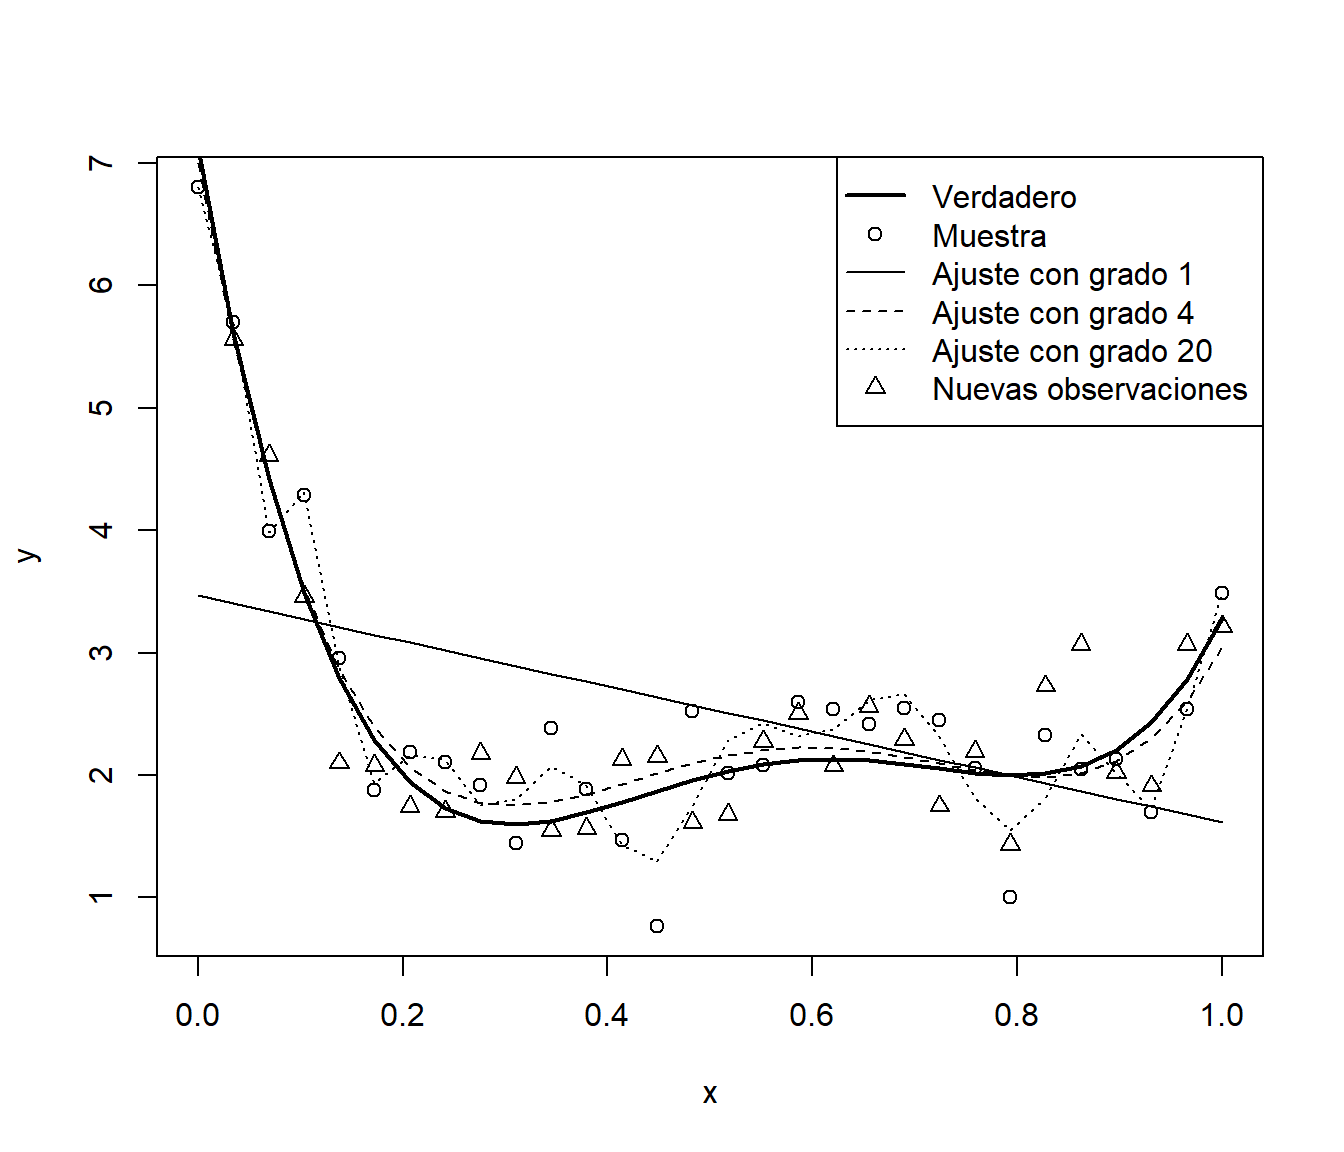
\includegraphics[width=0.8\linewidth]{01-introduccion_files/figure-latex/polyfit2-1} 

}

\caption{Muestra con ajustes polinómicos con distinta complejidad y nuevas observaciones.}\label{fig:polyfit2}
\end{figure}

\begin{Shaded}
\begin{Highlighting}[]
\NormalTok{MSEP <-}\StringTok{ }\KeywordTok{sapply}\NormalTok{(}\KeywordTok{list}\NormalTok{(}\DataTypeTok{fit1 =}\NormalTok{ fit1, }\DataTypeTok{fit2 =}\NormalTok{ fit2, }\DataTypeTok{fit3 =}\NormalTok{ fit3), }
               \ControlFlowTok{function}\NormalTok{(x) }\KeywordTok{mean}\NormalTok{((y.new }\OperatorTok{-}\StringTok{ }\KeywordTok{fitted}\NormalTok{(x))}\OperatorTok{^}\DecValTok{2}\NormalTok{))}
\NormalTok{MSEP}
\end{Highlighting}
\end{Shaded}

\begin{verbatim}
##      fit1      fit2      fit3 
## 1.4983208 0.1711238 0.2621064
\end{verbatim}

Como ejemplo adicional, para evitar el efecto de la aleatoriedad de la
muestra, en el siguiente código se simulan 100 muestras del proceso
anterior a las que se les ajustan modelos polinómicos variando el grado
de 1 a 20. Posteriormente se evalua la precisión en la muestra empleada
en el ajuste y en un nuevo conjunto de datos procedente de la misma
población.

\begin{Shaded}
\begin{Highlighting}[]
\NormalTok{nsim <-}\StringTok{ }\DecValTok{100}
\KeywordTok{set.seed}\NormalTok{(}\DecValTok{1}\NormalTok{)}
\NormalTok{grado.max <-}\StringTok{ }\DecValTok{20}
\NormalTok{grados <-}\StringTok{ }\KeywordTok{seq_len}\NormalTok{(grado.max) }
\NormalTok{mse <-}\StringTok{ }\NormalTok{mse.new <-}\StringTok{ }\KeywordTok{matrix}\NormalTok{(}\DataTypeTok{nrow =}\NormalTok{ grado.max, }\DataTypeTok{ncol =}\NormalTok{ nsim) }\CommentTok{# Error cuadrático medio}
\ControlFlowTok{for}\NormalTok{(i }\ControlFlowTok{in} \KeywordTok{seq_len}\NormalTok{(nsim)) \{}
\NormalTok{  y <-}\StringTok{ }\NormalTok{mu }\OperatorTok{+}\StringTok{ }\KeywordTok{rnorm}\NormalTok{(n, }\DecValTok{0}\NormalTok{, sd)}
\NormalTok{  y.new <-}\StringTok{ }\NormalTok{mu }\OperatorTok{+}\StringTok{ }\KeywordTok{rnorm}\NormalTok{(n, }\DecValTok{0}\NormalTok{, sd)}
  \ControlFlowTok{for}\NormalTok{ (grado }\ControlFlowTok{in}\NormalTok{ grados) \{ }\CommentTok{# grado <- 1}
\NormalTok{    fit <-}\StringTok{ }\KeywordTok{lm}\NormalTok{(y }\OperatorTok{~}\StringTok{ }\KeywordTok{poly}\NormalTok{(x, grado))}
\NormalTok{    mse[grado, i] <-}\StringTok{ }\KeywordTok{mean}\NormalTok{(}\KeywordTok{residuals}\NormalTok{(fit)}\OperatorTok{^}\DecValTok{2}\NormalTok{)}
\NormalTok{    mse.new[grado, i] <-}\StringTok{ }\KeywordTok{mean}\NormalTok{((y.new }\OperatorTok{-}\StringTok{ }\KeywordTok{fitted}\NormalTok{(fit))}\OperatorTok{^}\DecValTok{2}\NormalTok{)}
\NormalTok{  \}}
\NormalTok{\}}
\CommentTok{# Simulaciones}
\KeywordTok{matplot}\NormalTok{(grados, mse, }\DataTypeTok{type =} \StringTok{"l"}\NormalTok{, }\DataTypeTok{col =} \StringTok{"lightgray"}\NormalTok{, }\DataTypeTok{lty =} \DecValTok{1}\NormalTok{, }\DataTypeTok{ylim =} \KeywordTok{c}\NormalTok{(}\DecValTok{0}\NormalTok{, }\DecValTok{2}\NormalTok{),}
        \DataTypeTok{xlab =} \StringTok{"Grado del polinomio (complejidad)"}\NormalTok{,}
        \DataTypeTok{ylab =} \StringTok{"Error cuadrático medio"}\NormalTok{)}
\KeywordTok{matlines}\NormalTok{(grados, mse.new, }\DataTypeTok{type =} \StringTok{"l"}\NormalTok{, }\DataTypeTok{lty =} \DecValTok{2}\NormalTok{, }\DataTypeTok{col =} \StringTok{"lightgray"}\NormalTok{) }
\CommentTok{# Global}
\NormalTok{precision <-}\StringTok{ }\KeywordTok{rowMeans}\NormalTok{(mse)}
\NormalTok{precision.new <-}\StringTok{ }\KeywordTok{rowMeans}\NormalTok{(mse.new)}
\KeywordTok{lines}\NormalTok{(grados, precision, }\DataTypeTok{lwd =} \DecValTok{2}\NormalTok{)}
\KeywordTok{lines}\NormalTok{(grados, precision.new, }\DataTypeTok{lty =} \DecValTok{2}\NormalTok{, }\DataTypeTok{lwd =} \DecValTok{2}\NormalTok{)}
\KeywordTok{abline}\NormalTok{(}\DataTypeTok{h =}\NormalTok{ sd}\OperatorTok{^}\DecValTok{2}\NormalTok{, }\DataTypeTok{lty =} \DecValTok{3}\NormalTok{)}
\KeywordTok{abline}\NormalTok{(}\DataTypeTok{v =} \DecValTok{4}\NormalTok{, }\DataTypeTok{lty =} \DecValTok{3}\NormalTok{)}
\KeywordTok{legend}\NormalTok{(}\StringTok{"topright"}\NormalTok{, }\DataTypeTok{legend =} \KeywordTok{c}\NormalTok{(}\StringTok{"Muestras"}\NormalTok{, }\StringTok{"Nuevas observaciones"}\NormalTok{), }\DataTypeTok{lty =} \KeywordTok{c}\NormalTok{(}\DecValTok{1}\NormalTok{, }\DecValTok{2}\NormalTok{))}
\end{Highlighting}
\end{Shaded}

\begin{figure}[!htb]

{\centering 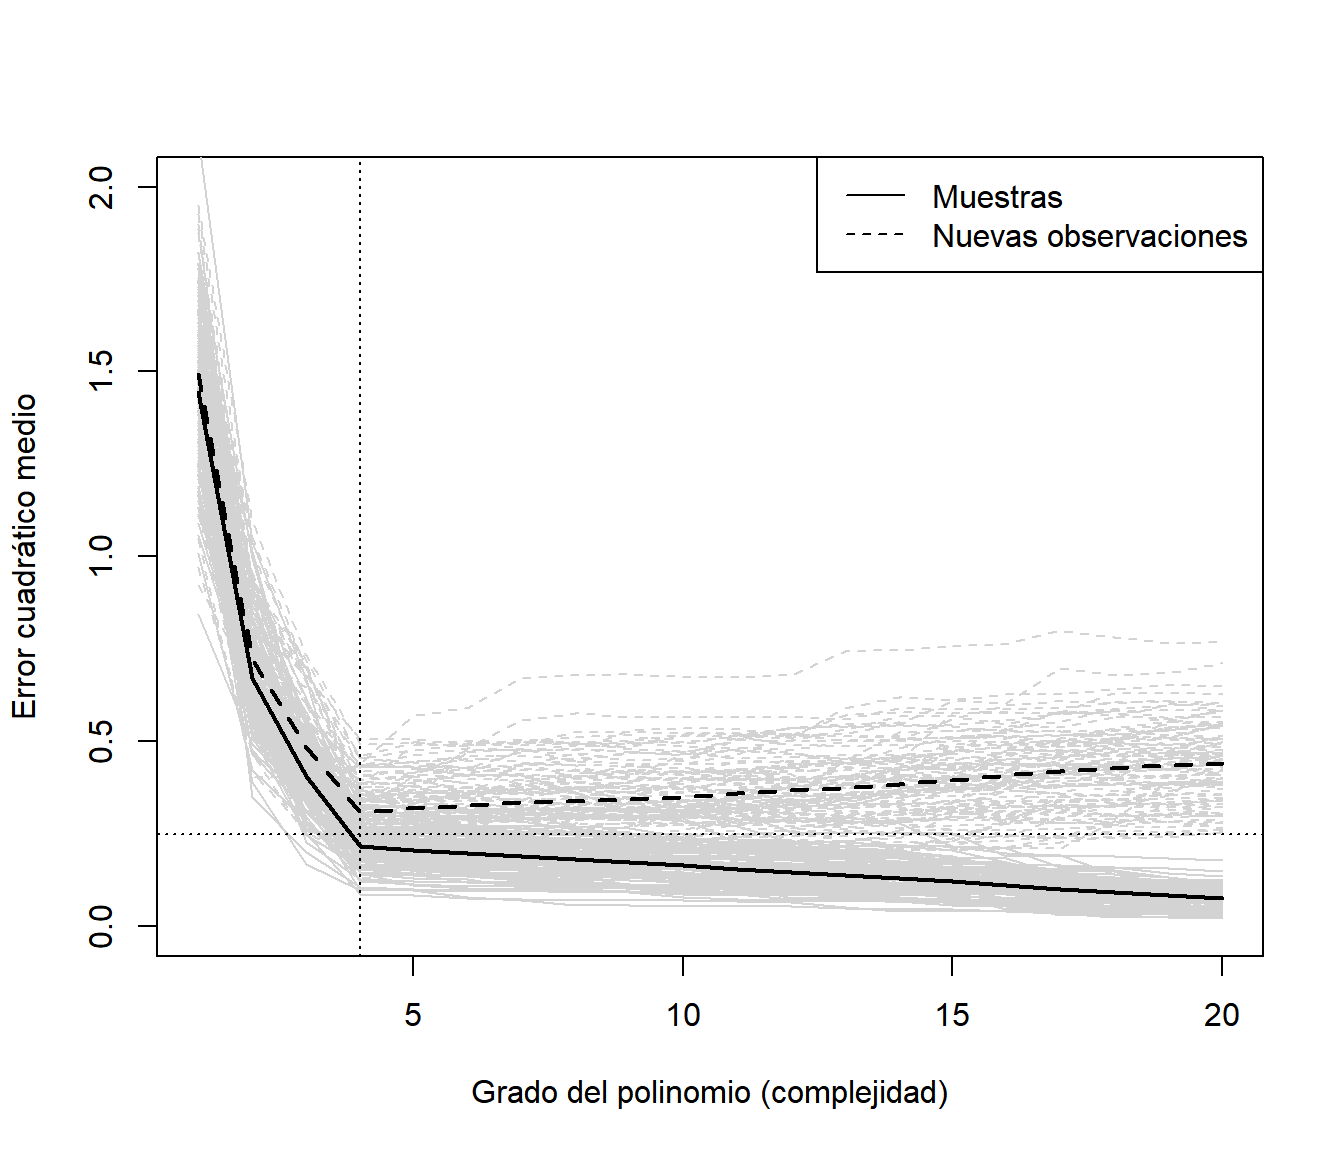
\includegraphics[width=0.8\linewidth]{01-introduccion_files/figure-latex/polyfitsim-1} 

}

\caption{Precisiones (errores cuadráticos medios) de ajustes polinómicos variando la complejidad, en las muestras empleadas en el ajuste y en nuevas observaciones (simulados).}\label{fig:polyfitsim}
\end{figure}

Como se puede observar en la Figura \ref{fig:polyfitsim} los errores de
entrenamiento disminuyen a medida que aumenta la complejidad del modelo.
Sin embargo los errores de predicción en nuevas observaciones primero
disminuyen hasta alcanzar un mínimo, marcado por la línea de puntos
vertical que se corresponde con el modelo de grado 4, y después aumentan
(la línea de puntos horizontal es la varianza del proceso; el error
cuadrático medio de predicción asintótico). La línea vertical representa
el equilibrio entre el sesgo y la varianza. Considerando un valor de
complejidad a la izquierda de esa línea tendríamos infraajuste (mayor
sesgo y menor varianza) y a la derecha sobreajuste (menor sesgo y mayor
varianza).

Desde un punto de vista más formal, considerando el modelo
\eqref{eq:modelogeneral} y una función de pérdidas cuadrática, el
predictor óptimo (desconocido) sería la media condicional
\(m(\mathbf{x}) = E\left( \left. Y\right\vert_{\mathbf{X}=\mathbf{x}} \right)\)\footnote{Se
  podrían considerar otras funciones de pérdida, por ejemplo con la
  distancia \(L_1\) sería la mediana condicional, pero las
  consideraciones serían análogas.}. Por tanto los predictores serían
realmente estimaciones de la función de regresión,
\(\hat Y(\mathbf{x}) = \hat m(\mathbf{x})\) y podemos expresar la media
del error cuadrático de predicción en términos del sesgo y la varianza:
\[
\begin{aligned}
E \left( Y(\mathbf{x}_0) - \hat Y(\mathbf{x}_0) \right)^2 & = E \left( m(\mathbf{x}_0) + \varepsilon - \hat m(\mathbf{x}_0) \right)^2 = E \left( m(\mathbf{x}_0) - \hat m(\mathbf{x}_0) \right)^2 + \sigma^2 \\
& = E^2 \left( m(\mathbf{x}_0) - \hat m(\mathbf{x}_0) \right) + Var\left( \hat m(\mathbf{x}_0) \right) + \sigma^2 \\
& = \text{sesgo}^2 + \text{varianza} + \text{error irreducible}
\end{aligned}
\] donde \(\mathbf{x}_0\) hace referencia al vector de valores de las
variables explicativas de una nueva observación (no empleada en la
construcción del predictor).

En general, al aumentar la complejidad disminuye el sesgo y aumenta la
varianza (y viceversa). Esto es lo que se conoce como el dilema o
compromiso entre el sesgo y la varianza (\emph{bias-variance tradeoff}).
La recomendación sería por tanto seleccionar los hiperparámetros (el
modelo final) tratando de que haya un equilibrio entre el sesgo y la
varianza.

\subsection{Datos de entrenamiento y datos de
test}\label{entrenamiento-test}

Como se mostró en la sección anterior hay que tener mucho cuidado si se
pretende evaluar la precisión de las predicciones empleando la muestra
de entrenamiento.

Si el número de observaciones no es muy grande, se puede entrenar el
modelo con todos los datos y emplear técnicas de remuestreo para evaluar
la precisión (típicamente validación cruzada o bootstrap). Habría que
asegurase de que el procedimiento de remuestreo empleado es adecuado
(por ejemplo, la presencia de dependencia requeriría de métodos más
sofisticados).

Sin embargo, si el número de obervaciones es grande, se suele emplear el
procedimiento tradicional en ML, que consiste en particionar la base de
datos en 2 (o incluso en 3) conjuntos (disjuntos):

\begin{itemize}
\item
  Conjunto de datos de entrenamiento (o aprendizaje) para construir los
  modelos.
\item
  Conjunto de datos de test para evaluar el rendimiento de los modelos.
\end{itemize}

Los datos de test deberían utilizarse únicamente para evaluar los
modelos finales, no se deberían emplear para seleccionar
hiperparámetros. Para seleccionalos se podría volver a particionar los
datos de entrenamiento, es decir, dividir la muestra en tres
subconjuntos: datos de entrenamiento, de validación y de test (por
ejemplo considerando un 70\%, 15\% y 15\% de las observaciones,
respectivamente). Para cada combinación de hiperparámetros se ajustaría
el correspondiente modelo con los datos de entrenamiento, se emplearían
los de validación para evaluarlos y posteriormente seleccionar los
valores ``óptimos''. Por último, se emplean los datos de test para
evaluar el rendimiento del modelo seleccionado. No obstante, lo más
habitual es seleccionar los hiperparámetros empleando validación cruzada
(o otro tipo de remuestreo) en la muestra de entrenamiento, en lugar de
considerar una muestra adicional de validación. En la siguiente sección
se describirá esta última aproximación.

En R se puede realizar el particionamiento de los datos empleando la
función \texttt{sample()} del paquete base (otra alternativa sería
emplear la función \texttt{createDataPartition} del paquete
\texttt{caret} como se describe en la Sección \ref{caret}). Típicamente
se selecciona el 80\% de los datos como muestra de entrenamiento y el
20\% restante como muestra de test, aunque esto dependería del número de
datos.

Como ejemplo consideraremos el conjunto de datos \texttt{Boston} del
paquete \texttt{MASS} que contiene, entre otros datos, la valoración de
las viviendas (\texttt{medv}, mediana de los valores de las viviendas
ocupadas, en miles de dólares) y el porcentaje de población con ``menor
estatus'' (\texttt{lstat}) en los suburbios de Boston. Podemos contruir
las muestras de entrenamiento (80\%) y de test (20\%) con el siguiente
código:

\begin{Shaded}
\begin{Highlighting}[]
\KeywordTok{data}\NormalTok{(Boston, }\DataTypeTok{package =} \StringTok{"MASS"}\NormalTok{)}
\CommentTok{# ?Boston}
\KeywordTok{set.seed}\NormalTok{(}\DecValTok{1}\NormalTok{)}
\NormalTok{nobs <-}\StringTok{ }\KeywordTok{nrow}\NormalTok{(Boston)}
\NormalTok{itrain <-}\StringTok{ }\KeywordTok{sample}\NormalTok{(nobs, }\FloatTok{0.8} \OperatorTok{*}\StringTok{ }\NormalTok{nobs)}
\NormalTok{train <-}\StringTok{ }\NormalTok{Boston[itrain, ]}
\NormalTok{test <-}\StringTok{ }\NormalTok{Boston[}\OperatorTok{-}\NormalTok{itrain, ]}
\end{Highlighting}
\end{Shaded}

\subsection{Validación cruzada}\label{cv}

Como ya se comentó, una herramienta para evaluar la calidad predictiva
de un modelo es la \emph{validación cruzada}, que permite cuantificar el
error de predicción utilizando una única muestra de datos.

En su versión más simple, validación cruzada dejando uno fuera
(\emph{Leave-one-out cross-validation}, LOOCV), para cada observación de
la muestra se realiza un ajuste empleando el resto de observaciones, y
se mide el error de predicción en esa observación (único dato no
utilizado en el ajuste del modelo). Finalmente, combinando todos los
errores individuales se puede obtener medidas globales del error de
predicción (o aproximar características de su distribución).

El método de LOOCV requeriría, en principio (ver comentarios más
adelante), el ajuste de un modelo para cada observación por lo que
pueden aparecer problemas computacionales si el conjunto de datos es
grande. En este caso se suele emplear grupos de observaciones en lugar
de observaciones individuales. Si se particiona el conjunto de datos en
\emph{k} grupos, típicamente 10 o 5 grupos, se denomina \emph{k-fold
cross-validation} (LOOCV sería un caso particular considerando un número
de grupos igual al número de observaciones). Hay muchas variaciones de
este método, entre ellas particionar repetidamente de forma aleatoria
los datos en un conjunto de entrenamiento y otro de validación (de esta
forma algunas observaciones podrían aparecer repetidas veces y otras
ninguna en las muestras de validación).

Continuando con el ejemplo anterior, supongamos que queremos emplear
regresión polinómica para explicar la valoración de las viviendas
(\texttt{medv}) a partir del ``estatus'' de los residentes
(\texttt{lstat}). Al igual que se hizo en la Sección
\ref{bias-variance}, consideraremos el grado del polinomio como un
hiperparámetro.

\begin{Shaded}
\begin{Highlighting}[]
\KeywordTok{plot}\NormalTok{(medv }\OperatorTok{~}\StringTok{ }\NormalTok{lstat, }\DataTypeTok{data =}\NormalTok{ train)}
\end{Highlighting}
\end{Shaded}

\begin{center}\includegraphics[width=0.8\linewidth]{01-introduccion_files/figure-latex/unnamed-chunk-4-1} \end{center}

Podríamos emplear la siguiente función que devuelve para cada
observación (fila) de una muestra de entrenamiento, el error de
predicción en esa observación ajustando un modelo lineal con todas las
demás observaciones:

\begin{Shaded}
\begin{Highlighting}[]
\NormalTok{cv.lm0 <-}\StringTok{ }\ControlFlowTok{function}\NormalTok{(formula, datos) \{}
\NormalTok{    n <-}\StringTok{ }\KeywordTok{nrow}\NormalTok{(datos)}
\NormalTok{    cv.res <-}\StringTok{ }\KeywordTok{numeric}\NormalTok{(n)}
    \ControlFlowTok{for}\NormalTok{ (i }\ControlFlowTok{in} \DecValTok{1}\OperatorTok{:}\NormalTok{n) \{}
\NormalTok{        modelo <-}\StringTok{ }\KeywordTok{lm}\NormalTok{(formula, datos[}\OperatorTok{-}\NormalTok{i, ])}
\NormalTok{        cv.pred <-}\StringTok{ }\KeywordTok{predict}\NormalTok{(modelo, }\DataTypeTok{newdata =}\NormalTok{ datos[i, ])}
\NormalTok{        cv.res[i] <-}\StringTok{ }\NormalTok{cv.pred }\OperatorTok{-}\StringTok{ }\NormalTok{datos[i, ]}
\NormalTok{    \}}
    \KeywordTok{return}\NormalTok{(cv.res)}
\NormalTok{\}}
\end{Highlighting}
\end{Shaded}

La función anterior no es muy eficiente, pero podría modificarse
fácilmente para emplear otros métodos de regresión\footnote{También
  puede ser de interés la función \texttt{cv.glm()} del paquete
  \texttt{boot}.}. En el caso de regresión lineal múltiple (y de otros
modelos lineales), se pueden obtener fácilmente las predicciones
eliminando una de las observaciones a partir del ajuste con todos los
datos. Por ejemplo, en lugar de la anterior sería preferible emplear la
siguiente función (ver \texttt{?rstandard}):

\begin{Shaded}
\begin{Highlighting}[]
\NormalTok{cv.lm <-}\StringTok{ }\ControlFlowTok{function}\NormalTok{(formula, datos) \{}
\NormalTok{    modelo <-}\StringTok{ }\KeywordTok{lm}\NormalTok{(formula, datos)}
    \KeywordTok{return}\NormalTok{(}\KeywordTok{rstandard}\NormalTok{(modelo, }\DataTypeTok{type =} \StringTok{"predictive"}\NormalTok{))}
\NormalTok{\}}
\end{Highlighting}
\end{Shaded}

Empleando esta función, podemos calcular una medida del error de
predicción de validación cruzada (en este caso el \emph{error cuadrático
medio}) para cada valor del hiperparámetro (grado del ajuste polinómico)
y seleccionar el que lo minimiza.

\begin{Shaded}
\begin{Highlighting}[]
\NormalTok{grado.max <-}\StringTok{ }\DecValTok{10}
\NormalTok{grados <-}\StringTok{ }\KeywordTok{seq_len}\NormalTok{(grado.max) }
\NormalTok{cv.mse <-}\StringTok{ }\NormalTok{cv.mse.sd <-}\StringTok{ }\KeywordTok{numeric}\NormalTok{(grado.max)}
\ControlFlowTok{for}\NormalTok{(grado }\ControlFlowTok{in}\NormalTok{ grados)\{}
\NormalTok{  cv.res <-}\StringTok{ }\KeywordTok{cv.lm}\NormalTok{(medv }\OperatorTok{~}\StringTok{ }\KeywordTok{poly}\NormalTok{(lstat, grado), train)}
\NormalTok{  se <-}\StringTok{ }\NormalTok{cv.res}\OperatorTok{^}\DecValTok{2}
\NormalTok{  cv.mse[grado] <-}\StringTok{ }\KeywordTok{mean}\NormalTok{(se)}
\NormalTok{  cv.mse.sd[grado] <-}\StringTok{ }\KeywordTok{sd}\NormalTok{(se)}\OperatorTok{/}\KeywordTok{sqrt}\NormalTok{(}\KeywordTok{length}\NormalTok{(se))}
\NormalTok{\}}
\KeywordTok{plot}\NormalTok{(grados, cv.mse, }\DataTypeTok{ylim =} \KeywordTok{c}\NormalTok{(}\DecValTok{25}\NormalTok{, }\DecValTok{45}\NormalTok{),}
  \DataTypeTok{xlab =} \StringTok{"Grado del polinomio (complejidad)"}\NormalTok{)}
\CommentTok{# Valor óptimo}
\NormalTok{imin.mse <-}\StringTok{ }\KeywordTok{which.min}\NormalTok{(cv.mse)}
\NormalTok{grado.op <-}\StringTok{ }\NormalTok{grados[imin.mse]}
\KeywordTok{points}\NormalTok{(grado.op, cv.mse[imin.mse], }\DataTypeTok{pch =} \DecValTok{16}\NormalTok{)}
\end{Highlighting}
\end{Shaded}

\begin{center}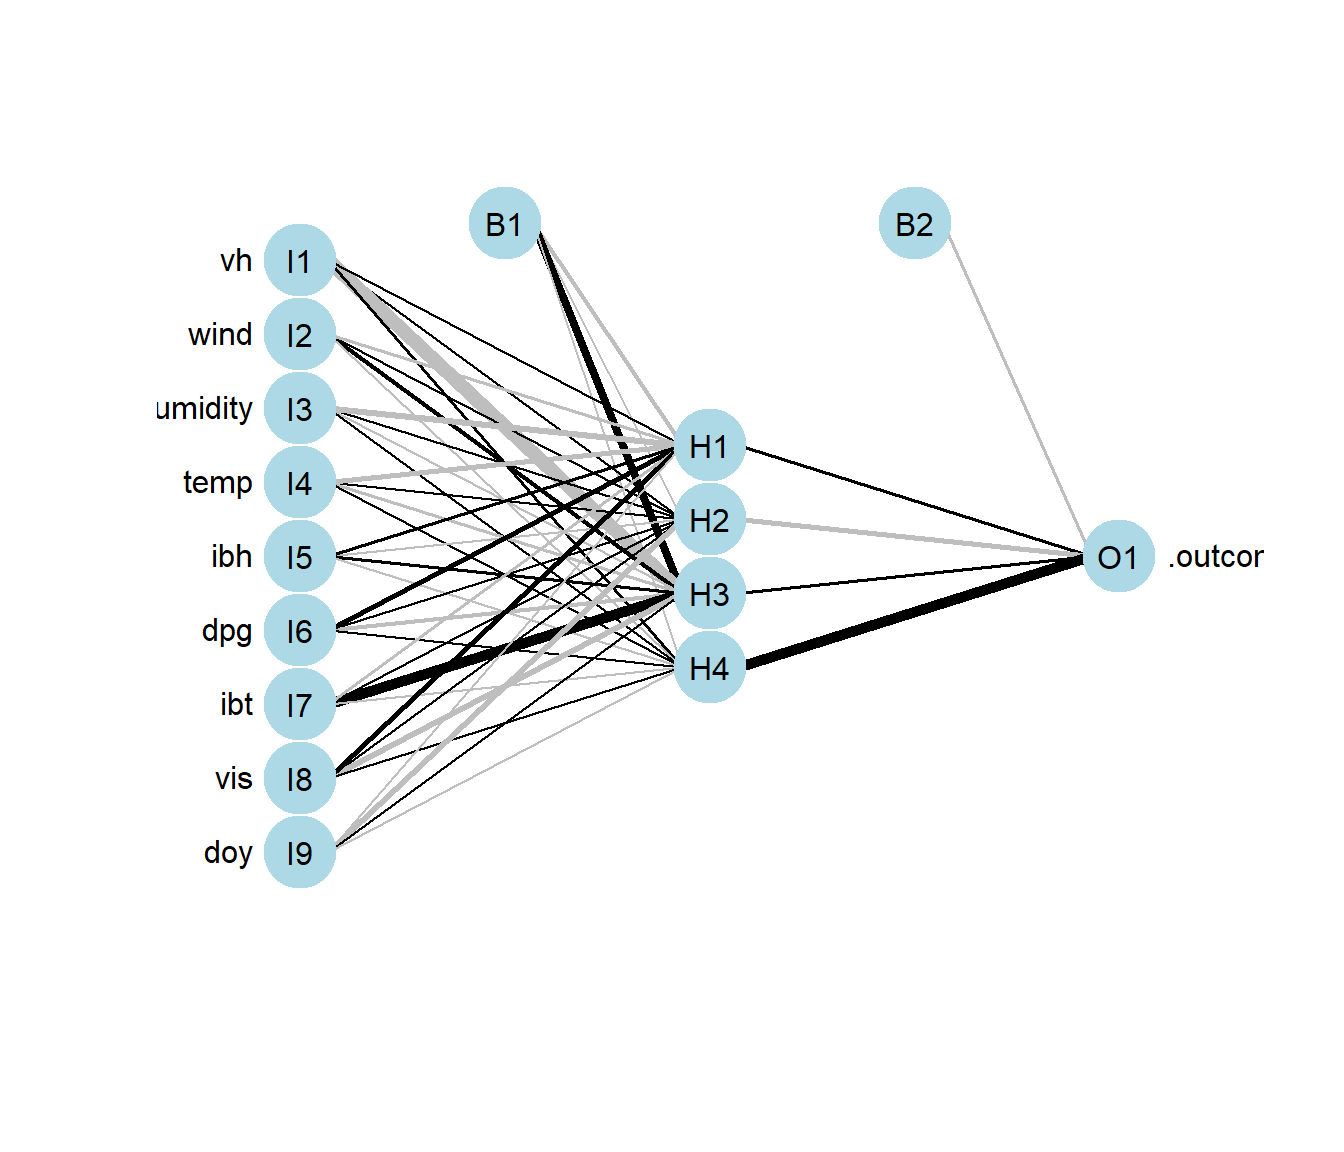
\includegraphics[width=0.8\linewidth]{01-introduccion_files/figure-latex/unnamed-chunk-7-1} \end{center}

\begin{Shaded}
\begin{Highlighting}[]
\NormalTok{grado.op}
\end{Highlighting}
\end{Shaded}

\begin{verbatim}
## [1] 5
\end{verbatim}

En lugar de emplear los valores óptimos de los hiperparámetros, Breiman
\emph{et al.} (1984) propusieron la regla de ``un error estándar'' para
seleccionar la complejidad del modelo. La idea es que estamos trabajando
con estimaciones de la precisión y pueden presentar variabilidad, por lo
que la sugerencia es seleccionar el modelo más simple\footnote{Suponiendo
  que los modelos se pueden ordenar del más simple al más complejo.}
dentro de un error estándar de la precisión del modelo correspondiente
al valor óptimo (se consideraría que no hay diferencias significativas
en la precisión; además, se mitigaría el efecto de la variabilidad
debida a aleatoriedad/semilla).

\begin{Shaded}
\begin{Highlighting}[]
\KeywordTok{plot}\NormalTok{(grados, cv.mse, }\DataTypeTok{ylim =} \KeywordTok{c}\NormalTok{(}\DecValTok{25}\NormalTok{, }\DecValTok{45}\NormalTok{))}
\KeywordTok{segments}\NormalTok{(grados, cv.mse }\OperatorTok{-}\StringTok{ }\NormalTok{cv.mse.sd, grados, cv.mse }\OperatorTok{+}\StringTok{ }\NormalTok{cv.mse.sd)}
\CommentTok{# Límite superior "oneSE rule" y complejidad mínima por debajo de ese valor}
\NormalTok{upper.cv.mse <-}\StringTok{ }\NormalTok{cv.mse[imin.mse] }\OperatorTok{+}\StringTok{ }\NormalTok{cv.mse.sd[imin.mse]}
\KeywordTok{abline}\NormalTok{(}\DataTypeTok{h =}\NormalTok{ upper.cv.mse, }\DataTypeTok{lty =} \DecValTok{2}\NormalTok{)}
\NormalTok{imin.1se <-}\StringTok{ }\KeywordTok{min}\NormalTok{(}\KeywordTok{which}\NormalTok{(cv.mse }\OperatorTok{<=}\StringTok{ }\NormalTok{upper.cv.mse))}
\NormalTok{grado.1se <-}\StringTok{ }\NormalTok{grados[imin.1se]}
\KeywordTok{points}\NormalTok{(grado.1se, cv.mse[imin.1se], }\DataTypeTok{pch =} \DecValTok{16}\NormalTok{)}
\end{Highlighting}
\end{Shaded}

\begin{center}\includegraphics[width=0.8\linewidth]{01-introduccion_files/figure-latex/unnamed-chunk-8-1} \end{center}

\begin{Shaded}
\begin{Highlighting}[]
\NormalTok{grado.1se}
\end{Highlighting}
\end{Shaded}

\begin{verbatim}
## [1] 2
\end{verbatim}

\begin{Shaded}
\begin{Highlighting}[]
\KeywordTok{plot}\NormalTok{(medv }\OperatorTok{~}\StringTok{ }\NormalTok{lstat, }\DataTypeTok{data =}\NormalTok{ train)}
\NormalTok{fit.op <-}\StringTok{ }\KeywordTok{lm}\NormalTok{(medv }\OperatorTok{~}\StringTok{ }\KeywordTok{poly}\NormalTok{(lstat, grado.op), train)}
\NormalTok{fit.1se <-}\StringTok{ }\KeywordTok{lm}\NormalTok{(medv }\OperatorTok{~}\StringTok{ }\KeywordTok{poly}\NormalTok{(lstat, grado.1se), train)}
\NormalTok{newdata <-}\StringTok{ }\KeywordTok{data.frame}\NormalTok{(}\DataTypeTok{lstat =} \KeywordTok{seq}\NormalTok{(}\DecValTok{0}\NormalTok{, }\DecValTok{40}\NormalTok{, }\DataTypeTok{len =} \DecValTok{100}\NormalTok{))}
\KeywordTok{lines}\NormalTok{(newdata}\OperatorTok{$}\NormalTok{lstat, }\KeywordTok{predict}\NormalTok{(fit.op, }\DataTypeTok{newdata =}\NormalTok{ newdata))}
\KeywordTok{lines}\NormalTok{(newdata}\OperatorTok{$}\NormalTok{lstat, }\KeywordTok{predict}\NormalTok{(fit.1se, }\DataTypeTok{newdata =}\NormalTok{ newdata), }\DataTypeTok{lty =} \DecValTok{2}\NormalTok{)}
\KeywordTok{legend}\NormalTok{(}\StringTok{"topright"}\NormalTok{, }\DataTypeTok{legend =} \KeywordTok{c}\NormalTok{(}\KeywordTok{paste}\NormalTok{(}\StringTok{"Grado óptimo:"}\NormalTok{, grado.op), }\KeywordTok{paste}\NormalTok{(}\StringTok{"oneSE rule:"}\NormalTok{, grado.1se)), }
       \DataTypeTok{lty =} \KeywordTok{c}\NormalTok{(}\DecValTok{1}\NormalTok{, }\DecValTok{2}\NormalTok{))}
\end{Highlighting}
\end{Shaded}

\begin{center}\includegraphics[width=0.8\linewidth]{01-introduccion_files/figure-latex/unnamed-chunk-9-1} \end{center}

\subsection{Evaluación de un método de regresión}\label{eval-reg}

Para estudiar la precisión de las predicciones de un método de regresión
se evalúa el modelo en el conjunto de datos de test y se comparan las
predicciones frente a los valores reales.

Si generamos un gráfico de dispersión de observaciones frente a
predicciones, los puntos deberían estar en torno a la recta \(y=x\)
(línea continua).

\begin{Shaded}
\begin{Highlighting}[]
\NormalTok{obs <-}\StringTok{ }\NormalTok{test}\OperatorTok{$}\NormalTok{medv}
\NormalTok{pred <-}\StringTok{ }\KeywordTok{predict}\NormalTok{(fit.op, }\DataTypeTok{newdata =}\NormalTok{ test)}

\KeywordTok{plot}\NormalTok{(pred, obs, }\DataTypeTok{main =} \StringTok{"Observado frente a predicciones"}\NormalTok{,}
     \DataTypeTok{xlab =} \StringTok{"Predicción", ylab = "}\NormalTok{Observado}\StringTok{")}
\StringTok{abline(a = 0, b = 1)}
\StringTok{res <- lm(obs ~ pred)}
\StringTok{# summary(res)}
\StringTok{abline(res, lty = 2)}
\end{Highlighting}
\end{Shaded}

\begin{center}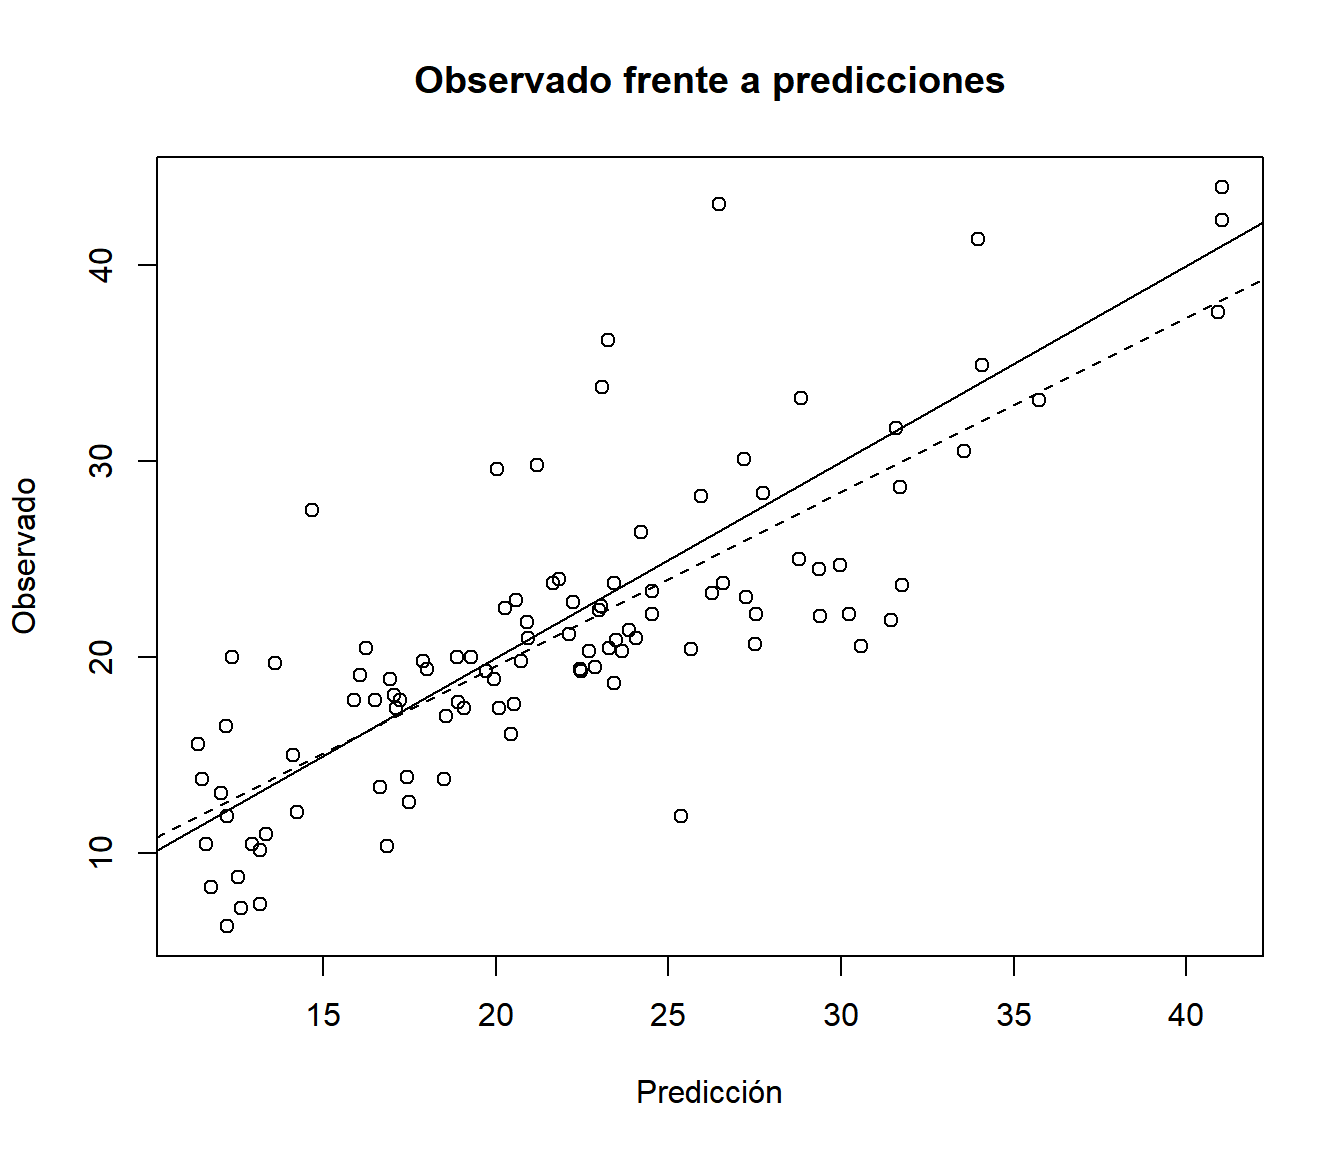
\includegraphics[width=0.8\linewidth]{01-introduccion_files/figure-latex/obs-pred-plot-1} \end{center}

También es habitual calcular distintas medidas de error. Por ejemplo,
podríamos emplear la función \texttt{postResample()} del paquete
\texttt{caret}:

\begin{Shaded}
\begin{Highlighting}[]
\NormalTok{caret}\OperatorTok{::}\KeywordTok{postResample}\NormalTok{(pred, obs)}
\end{Highlighting}
\end{Shaded}

\begin{verbatim}
##      RMSE  Rsquared       MAE 
## 4.8526718 0.6259583 3.6671847
\end{verbatim}

La función anterior, además de las medidas de error habituales (que
dependen en su mayoría de la escala de la variable respuesta) calcula un
\emph{pseudo R-cuadrado}. En este paquete (también en \texttt{rattle})
se emplea uno de los más utilizados, el cuadrado del coeficiente de
correlación entre las predicciones y los valores observados (que se
corresponde con la línea discontinua en la figura anterior). Estos
valores se interpretarían como el coeficiente de determinación en
regresión lineal, debería ser próximo a 1. Hay otras alternativas (ver
Kvålseth, 1985), pero la idea es que deberían medir la proporción de
variabilidad de la respuesta explicada por el modelo, algo que en
general no es cierto con el anterior\footnote{Por ejemplo obtendríamos
  el mismo valor si desplazamos las predicciones sumando una constante
  (i.e.~no tiene en cuenta el sesgo).}. La recomendación sería emplear:
\[\tilde R^2 = 1 - \frac{\sum_{i=1}^n(y_i - \hat y_i)^2}{\sum_{i=1}^n(y_i - \bar y_i)^2}\]
implementado junto con otras medidas en la siguiente función:

\begin{Shaded}
\begin{Highlighting}[]
\NormalTok{accuracy <-}\StringTok{ }\ControlFlowTok{function}\NormalTok{(pred, obs, }\DataTypeTok{na.rm =} \OtherTok{FALSE}\NormalTok{, }
                     \DataTypeTok{tol =} \KeywordTok{sqrt}\NormalTok{(.Machine}\OperatorTok{$}\NormalTok{double.eps)) \{}
\NormalTok{  err <-}\StringTok{ }\NormalTok{obs }\OperatorTok{-}\StringTok{ }\NormalTok{pred     }\CommentTok{# Errores}
  \ControlFlowTok{if}\NormalTok{(na.rm) \{}
\NormalTok{    is.a <-}\StringTok{ }\OperatorTok{!}\KeywordTok{is.na}\NormalTok{(err)}
\NormalTok{    err <-}\StringTok{ }\NormalTok{err[is.a]}
\NormalTok{    obs <-}\StringTok{ }\NormalTok{obs[is.a]}
\NormalTok{  \}  }
\NormalTok{  perr <-}\StringTok{ }\DecValTok{100}\OperatorTok{*}\NormalTok{err}\OperatorTok{/}\KeywordTok{pmax}\NormalTok{(obs, tol)  }\CommentTok{# Errores porcentuales}
  \KeywordTok{return}\NormalTok{(}\KeywordTok{c}\NormalTok{(}
    \DataTypeTok{me =} \KeywordTok{mean}\NormalTok{(err),           }\CommentTok{# Error medio}
    \DataTypeTok{rmse =} \KeywordTok{sqrt}\NormalTok{(}\KeywordTok{mean}\NormalTok{(err}\OperatorTok{^}\DecValTok{2}\NormalTok{)), }\CommentTok{# Raíz del error cuadrático medio }
    \DataTypeTok{mae =} \KeywordTok{mean}\NormalTok{(}\KeywordTok{abs}\NormalTok{(err)),     }\CommentTok{# Error absoluto medio}
    \DataTypeTok{mpe =} \KeywordTok{mean}\NormalTok{(perr),         }\CommentTok{# Error porcentual medio}
    \DataTypeTok{mape =} \KeywordTok{mean}\NormalTok{(}\KeywordTok{abs}\NormalTok{(perr)),   }\CommentTok{# Error porcentual absoluto medio}
    \DataTypeTok{r.squared =} \DecValTok{1} \OperatorTok{-}\StringTok{ }\KeywordTok{sum}\NormalTok{(err}\OperatorTok{^}\DecValTok{2}\NormalTok{)}\OperatorTok{/}\KeywordTok{sum}\NormalTok{((obs }\OperatorTok{-}\StringTok{ }\KeywordTok{mean}\NormalTok{(obs))}\OperatorTok{^}\DecValTok{2}\NormalTok{) }\CommentTok{# Pseudo R-cuadrado}
\NormalTok{  ))}
\NormalTok{\}}
\KeywordTok{accuracy}\NormalTok{(pred, obs)}
\end{Highlighting}
\end{Shaded}

\begin{verbatim}
##         me       rmse        mae        mpe       mape  r.squared 
## -0.6731294  4.8526718  3.6671847 -8.2322506 19.7097373  0.6086704
\end{verbatim}

\begin{Shaded}
\begin{Highlighting}[]
\KeywordTok{accuracy}\NormalTok{(}\KeywordTok{predict}\NormalTok{(fit.1se, }\DataTypeTok{newdata =}\NormalTok{ test), obs)}
\end{Highlighting}
\end{Shaded}

\begin{verbatim}
##         me       rmse        mae        mpe       mape  r.squared 
## -0.9236280  5.2797360  4.1252053 -9.0029771 21.6512406  0.5367608
\end{verbatim}

\BeginKnitrBlock{exercise}
\protect\hypertarget{exr:train-validate-test}{}{\label{exr:train-validate-test}
}
\EndKnitrBlock{exercise}

Considerando de nuevo el ejemplo anterior, particionar la muestra en
datos de entrenamiento (70\%), de validación (15\%) y de test (15\%),
para entrenar los modelos polinómicos, seleccionar el grado óptimo (el
hiperparámetro) y evaluar las predicciones del modelo final,
respectivamente.

Podría ser de utilidad el siguiente código (basado en la aproximación de
\texttt{rattle}), que particiona los datos suponiendo que están
almacenados en el data.frame \texttt{df}:

\begin{Shaded}
\begin{Highlighting}[]
\NormalTok{df <-}\StringTok{ }\NormalTok{Boston}
\KeywordTok{set.seed}\NormalTok{(}\DecValTok{1}\NormalTok{)}
\NormalTok{nobs <-}\StringTok{ }\KeywordTok{nrow}\NormalTok{(df)}
\NormalTok{itrain <-}\StringTok{ }\KeywordTok{sample}\NormalTok{(nobs, }\FloatTok{0.7} \OperatorTok{*}\StringTok{ }\NormalTok{nobs)}
\NormalTok{inotrain <-}\StringTok{ }\KeywordTok{setdiff}\NormalTok{(}\KeywordTok{seq_len}\NormalTok{(nobs), itrain)}
\NormalTok{ivalidate <-}\StringTok{ }\KeywordTok{sample}\NormalTok{(inotrain, }\FloatTok{0.15} \OperatorTok{*}\StringTok{ }\NormalTok{nobs)}
\NormalTok{itest <-}\StringTok{ }\KeywordTok{setdiff}\NormalTok{(inotrain, ivalidate)}
\NormalTok{train <-}\StringTok{ }\NormalTok{df[itrain, ]}
\NormalTok{validate <-}\StringTok{ }\NormalTok{df[ivalidate, ]}
\NormalTok{test <-}\StringTok{ }\NormalTok{df[itest, ]}
\end{Highlighting}
\end{Shaded}

Alternativamente podríamos emplear la función \texttt{split()} creando
un factor que divida aleatoriamente los datos en tres grupos (versión
``simplificada'' de una propuesta en este
\href{https://stackoverflow.com/questions/36068963/r-how-to-split-a-data-frame-into-training-validation-and-test-sets}{post}):

\begin{Shaded}
\begin{Highlighting}[]
\KeywordTok{set.seed}\NormalTok{(}\DecValTok{1}\NormalTok{)}
\NormalTok{p <-}\StringTok{ }\KeywordTok{c}\NormalTok{(}\DataTypeTok{train =} \FloatTok{0.7}\NormalTok{, }\DataTypeTok{validate =} \FloatTok{0.15}\NormalTok{, }\DataTypeTok{test =} \FloatTok{0.15}\NormalTok{)}
\NormalTok{f <-}\StringTok{ }\KeywordTok{sample}\NormalTok{( }\KeywordTok{rep}\NormalTok{(}\KeywordTok{factor}\NormalTok{(}\KeywordTok{seq_along}\NormalTok{(p), }\DataTypeTok{labels =} \KeywordTok{names}\NormalTok{(p)),}
                 \DataTypeTok{times =} \KeywordTok{nrow}\NormalTok{(df)}\OperatorTok{*}\NormalTok{p}\OperatorTok{/}\KeywordTok{sum}\NormalTok{(p)) )}
\NormalTok{samples <-}\StringTok{ }\KeywordTok{suppressWarnings}\NormalTok{(}\KeywordTok{split}\NormalTok{(df, f))}
\KeywordTok{str}\NormalTok{(samples)}
\end{Highlighting}
\end{Shaded}

\begin{verbatim}
## List of 3
##  $ train   :'data.frame':    356 obs. of  14 variables:
##   ..$ crim   : num [1:356] 0.00632 0.02731 0.02729 0.02985 0.08829 ...
##   ..$ zn     : num [1:356] 18 0 0 0 12.5 12.5 12.5 12.5 12.5 0 ...
##   ..$ indus  : num [1:356] 2.31 7.07 7.07 2.18 7.87 7.87 7.87 7.87 7.87 8.14 ...
##   ..$ chas   : int [1:356] 0 0 0 0 0 0 0 0 0 0 ...
##   ..$ nox    : num [1:356] 0.538 0.469 0.469 0.458 0.524 0.524 0.524 0.524 0.524 0.538 ...
##   ..$ rm     : num [1:356] 6.58 6.42 7.18 6.43 6.01 ...
##   ..$ age    : num [1:356] 65.2 78.9 61.1 58.7 66.6 100 85.9 82.9 39 56.5 ...
##   ..$ dis    : num [1:356] 4.09 4.97 4.97 6.06 5.56 ...
##   ..$ rad    : int [1:356] 1 2 2 3 5 5 5 5 5 4 ...
##   ..$ tax    : num [1:356] 296 242 242 222 311 311 311 311 311 307 ...
##   ..$ ptratio: num [1:356] 15.3 17.8 17.8 18.7 15.2 15.2 15.2 15.2 15.2 21 ...
##   ..$ black  : num [1:356] 397 397 393 394 396 ...
##   ..$ lstat  : num [1:356] 4.98 9.14 4.03 5.21 12.43 ...
##   ..$ medv   : num [1:356] 24 21.6 34.7 28.7 22.9 16.5 18.9 18.9 21.7 19.9 ...
##  $ validate:'data.frame':    75 obs. of  14 variables:
##   ..$ crim   : num [1:75] 0.0324 0.6298 0.9884 0.9558 1.0025 ...
##   ..$ zn     : num [1:75] 0 0 0 0 0 0 0 75 75 0 ...
##   ..$ indus  : num [1:75] 2.18 8.14 8.14 8.14 8.14 8.14 5.96 2.95 2.95 6.91 ...
##   ..$ chas   : int [1:75] 0 0 0 0 0 0 0 0 0 0 ...
##   ..$ nox    : num [1:75] 0.458 0.538 0.538 0.538 0.538 0.538 0.499 0.428 0.428 0.448 ...
##   ..$ rm     : num [1:75] 7 5.95 5.81 6.05 6.67 ...
##   ..$ age    : num [1:75] 45.8 61.8 100 88.8 87.3 95 41.5 21.8 15.8 6.5 ...
##   ..$ dis    : num [1:75] 6.06 4.71 4.1 4.45 4.24 ...
##   ..$ rad    : int [1:75] 3 4 4 4 4 4 5 3 3 3 ...
##   ..$ tax    : num [1:75] 222 307 307 307 307 307 279 252 252 233 ...
##   ..$ ptratio: num [1:75] 18.7 21 21 21 21 21 19.2 18.3 18.3 17.9 ...
##   ..$ black  : num [1:75] 395 397 395 306 380 ...
##   ..$ lstat  : num [1:75] 2.94 8.26 19.88 17.28 11.98 ...
##   ..$ medv   : num [1:75] 33.4 20.4 14.5 14.8 21 13.1 21 30.8 34.9 24.7 ...
##  $ test    :'data.frame':    75 obs. of  14 variables:
##   ..$ crim   : num [1:75] 0.069 0.1446 0.2249 0.638 0.6719 ...
##   ..$ zn     : num [1:75] 0 12.5 12.5 0 0 0 0 90 0 0 ...
##   ..$ indus  : num [1:75] 2.18 7.87 7.87 8.14 8.14 ...
##   ..$ chas   : int [1:75] 0 0 0 0 0 0 0 0 0 0 ...
##   ..$ nox    : num [1:75] 0.458 0.524 0.524 0.538 0.538 0.538 0.499 0.403 0.413 0.413 ...
##   ..$ rm     : num [1:75] 7.15 6.17 6.38 6.1 5.81 ...
##   ..$ age    : num [1:75] 54.2 96.1 94.3 84.5 90.3 94.1 68.2 21.9 6.6 7.8 ...
##   ..$ dis    : num [1:75] 6.06 5.95 6.35 4.46 4.68 ...
##   ..$ rad    : int [1:75] 3 5 5 4 4 4 5 5 4 4 ...
##   ..$ tax    : num [1:75] 222 311 311 307 307 307 279 226 305 305 ...
##   ..$ ptratio: num [1:75] 18.7 15.2 15.2 21 21 21 19.2 17.9 19.2 19.2 ...
##   ..$ black  : num [1:75] 397 397 393 380 377 ...
##   ..$ lstat  : num [1:75] 5.33 19.15 20.45 10.26 14.81 ...
##   ..$ medv   : num [1:75] 36.2 27.1 15 18.2 16.6 12.7 18.9 35.4 24.2 22.8 ...
\end{verbatim}

\subsection{Evaluación de un método de clasificación}\label{eval-class}

Para estudiar la eficiencia de un método de clasificación supervisada
típicamente se obtienen las predicciones para el conjunto de datos de
test y se genera una tabla de contingencia, denominada \emph{matriz de
confusión}, con las predicciones frente a los valores reales.

En primer lugar consideraremos el caso de dos categorías. La matriz de
confusión será de la forma:

\begin{longtable}[]{@{}ccc@{}}
\toprule
Observado\textbackslash{}Predicción & Positivo & Negativo\tabularnewline
\midrule
\endhead
Verdadero & Verdaderos positivos (TP) & Falsos negativos
(FN)\tabularnewline
Falso & Falsos positivos (FP) & Verdaderos negativos (TN)\tabularnewline
\bottomrule
\end{longtable}

A partir de esta tabla se pueden obtener distintas medidas de la
precisión de las predicciones. Por ejemplo, dos de las más utilizadas
son la tasa de verdaderos positivos y la de verdaderos negativos (tasas
de acierto en positivos y negativos), también denominadas
\emph{sensibilidad} y \emph{especificidad}:

\begin{itemize}
\item
  Sensibilidad (\emph{sensitivity}, \emph{recall}, \emph{hit rate},
  \emph{true positive rate}; TPR):
  \[TPR = \frac{TP}{P} = \frac{TP}{TP+FN}\]
\item
  Especificidad (\emph{specificity}, \emph{true negative rate}; TNR):
  \[TNR = \frac{TN}{TN+FP}\]
\end{itemize}

La precisión global o tasa de aciertos (\emph{accuracy}; ACC) sería:
\[ACC = \frac{TP + TN}{P + N} = \frac{TP+TN}{TP+TN+FP+FN}\] Sin embargo
hay que tener cuidado con esta medida cuando las clases no están
balanceadas. Otras medidas de la precisión global que tratan de evitar
este problema son la \emph{precisión balanceada} (\emph{balanced
accuracy}, BA): \[BA = \frac{TPR + TNR}{2}\] (media aritmética de TPR y
TNR) o la \emph{puntuación F1} (\emph{F1 score}; media armónica de TPR y
el valor predictivo positivo, PPV, descrito más adelante):
\[F_1 = \frac{2TP}{2TP+FP+FN}\] Otra medida global es el coeficiente
kappa de Cohen, que compara la tasa de aciertos con la obtenida en una
clasificación al azar (un valor de 1 indicaría máxima precisión y 0 que
la precisión es igual a la que obtendríamos clasificando al azar;
empleando la tasa de positivos, denominada \emph{prevalencia}, para
predecir positivo).

También hay que tener cuidado las medidas que utilizan como estimación
de la probabilidad de positivo (\emph{prevalencia}) la tasa de positivos
en la muestra de test, como el valor (o índice) predictivo positivo
(\emph{precision}, \emph{positive predictive value}; PPV):
\[PPV = \frac{TP}{TP+FP}\] (que no debe ser confundido con la precisión
global ACC) y el valor predictivo negativo negativo (NPV):
\[NPV = \frac{TN}{TN+FN},\] si la muestra de test no refleja lo que
ocurre en la población (por ejemplo si la clase de interés está
sobrerrepresentada en la muestra). En estos casos habrá que
recalcularlos empleando estimaciones válidas de las probabilidades de la
clases (por ejemplo, en estos casos, la función
\texttt{caret::confusionMatrix()} permite establecer estimaciones
válidas mediante el argumento \texttt{prevalence}).

Como ejemplo emplearemos los datos anteriores de valoraciones de
viviendas y estatus de la población, considerando como respuesta una
nueva variable \texttt{fmedv} que clasifica las valoraciones en ``Bajo''
o ``Alto'' dependiendo de si \texttt{medv\ \textgreater{}\ 25}.

\begin{Shaded}
\begin{Highlighting}[]
\CommentTok{# data(Boston, package = "MASS")}
\NormalTok{datos <-}\StringTok{ }\NormalTok{Boston}
\NormalTok{datos}\OperatorTok{$}\NormalTok{fmedv <-}\StringTok{ }\KeywordTok{factor}\NormalTok{(datos}\OperatorTok{$}\NormalTok{medv }\OperatorTok{>}\StringTok{ }\DecValTok{25}\NormalTok{, }\DataTypeTok{labels =} \KeywordTok{c}\NormalTok{(}\StringTok{"Bajo"}\NormalTok{, }\StringTok{"Alto"}\NormalTok{)) }\CommentTok{# levels = c('FALSE', 'TRUE')}
\CommentTok{# En este caso las clases no están balanceadas}
\KeywordTok{table}\NormalTok{(datos}\OperatorTok{$}\NormalTok{fmedv)}
\end{Highlighting}
\end{Shaded}

\begin{verbatim}
## 
## Bajo Alto 
##  382  124
\end{verbatim}

\begin{Shaded}
\begin{Highlighting}[]
\NormalTok{caret}\OperatorTok{::}\KeywordTok{featurePlot}\NormalTok{(datos}\OperatorTok{$}\NormalTok{lstat, datos}\OperatorTok{$}\NormalTok{fmedv, }\DataTypeTok{plot =} \StringTok{"density"}\NormalTok{,}
            \DataTypeTok{labels =} \KeywordTok{c}\NormalTok{(}\StringTok{"lstat"}\NormalTok{, }\StringTok{"Density"}\NormalTok{), }\DataTypeTok{auto.key =} \OtherTok{TRUE}\NormalTok{)}
\end{Highlighting}
\end{Shaded}

\begin{center}\includegraphics[width=0.8\linewidth]{01-introduccion_files/figure-latex/unnamed-chunk-14-1} \end{center}

El siguiente código realiza la partición de los datos y posteriormente
ajusta un modelo de regresión logística en la muestra de entrenamiento
considerando \texttt{lstat} como única variable explicativa (en el
Capítulo 5 se darán más detalles sobre este tipo de modelos):

\begin{Shaded}
\begin{Highlighting}[]
\CommentTok{# Particionado de los datos}
\KeywordTok{set.seed}\NormalTok{(}\DecValTok{1}\NormalTok{)}
\NormalTok{nobs <-}\StringTok{ }\KeywordTok{nrow}\NormalTok{(datos)}
\NormalTok{itrain <-}\StringTok{ }\KeywordTok{sample}\NormalTok{(nobs, }\FloatTok{0.8} \OperatorTok{*}\StringTok{ }\NormalTok{nobs)}
\NormalTok{train <-}\StringTok{ }\NormalTok{datos[itrain, ]}
\NormalTok{test <-}\StringTok{ }\NormalTok{datos[}\OperatorTok{-}\NormalTok{itrain, ]}
\CommentTok{# Ajuste modelo}
\NormalTok{modelo <-}\StringTok{ }\KeywordTok{glm}\NormalTok{(fmedv }\OperatorTok{~}\StringTok{ }\NormalTok{lstat, }\DataTypeTok{family =}\NormalTok{ binomial, }\DataTypeTok{data =}\NormalTok{ train)}
\KeywordTok{summary}\NormalTok{(modelo)}
\end{Highlighting}
\end{Shaded}

\begin{verbatim}
## 
## Call:
## glm(formula = fmedv ~ lstat, family = binomial, data = train)
## 
## Deviance Residuals: 
##     Min       1Q   Median       3Q      Max  
## -1.9749  -0.4161  -0.0890   0.3785   3.6450  
## 
## Coefficients:
##             Estimate Std. Error z value Pr(>|z|)    
## (Intercept)  3.74366    0.47901   7.815 5.48e-15 ***
## lstat       -0.54231    0.06134  -8.842  < 2e-16 ***
## ---
## Signif. codes:  0 '***' 0.001 '**' 0.01 '*' 0.05 '.' 0.1 ' ' 1
## 
## (Dispersion parameter for binomial family taken to be 1)
## 
##     Null deviance: 460.84  on 403  degrees of freedom
## Residual deviance: 243.34  on 402  degrees of freedom
## AIC: 247.34
## 
## Number of Fisher Scoring iterations: 7
\end{verbatim}

En este caso podemos obtener las estimaciones de la probabilidad de la
segunda categoría empleando \texttt{predict()} con
\texttt{type\ =\ "response"}, a partir de las cuales podemos establecer
las predicciones como la categoría más probable:

\begin{Shaded}
\begin{Highlighting}[]
\NormalTok{obs <-}\StringTok{ }\NormalTok{test}\OperatorTok{$}\NormalTok{fmedv}
\NormalTok{p.est <-}\StringTok{ }\KeywordTok{predict}\NormalTok{(modelo, }\DataTypeTok{type =} \StringTok{"response"}\NormalTok{, }\DataTypeTok{newdata =}\NormalTok{ test)}
\NormalTok{pred <-}\StringTok{ }\KeywordTok{factor}\NormalTok{(p.est }\OperatorTok{>}\StringTok{ }\FloatTok{0.5}\NormalTok{, }\DataTypeTok{labels =} \KeywordTok{c}\NormalTok{(}\StringTok{"Bajo"}\NormalTok{, }\StringTok{"Alto"}\NormalTok{)) }\CommentTok{# levels = c('FALSE', 'TRUE')}
\end{Highlighting}
\end{Shaded}

Finalmente podemos obtener la matriz de confusión con el siguiente
código:

\begin{Shaded}
\begin{Highlighting}[]
\NormalTok{tabla <-}\StringTok{ }\KeywordTok{table}\NormalTok{(obs, pred)}
\CommentTok{# addmargins(tabla, FUN = list(Total = sum))}
\NormalTok{tabla}
\end{Highlighting}
\end{Shaded}

\begin{verbatim}
##       pred
## obs    Bajo Alto
##   Bajo   71   11
##   Alto    8   12
\end{verbatim}

\begin{Shaded}
\begin{Highlighting}[]
\CommentTok{# Porcentajes respecto al total}
\KeywordTok{print}\NormalTok{(}\DecValTok{100}\OperatorTok{*}\KeywordTok{prop.table}\NormalTok{(tabla), }\DataTypeTok{digits =} \DecValTok{2}\NormalTok{) }
\end{Highlighting}
\end{Shaded}

\begin{verbatim}
##       pred
## obs    Bajo Alto
##   Bajo 69.6 10.8
##   Alto  7.8 11.8
\end{verbatim}

\begin{Shaded}
\begin{Highlighting}[]
\CommentTok{# Porcentajes (de aciertos y fallos) por categorías}
\KeywordTok{print}\NormalTok{(}\DecValTok{100}\OperatorTok{*}\KeywordTok{prop.table}\NormalTok{(tabla, }\DecValTok{1}\NormalTok{), }\DataTypeTok{digits =} \DecValTok{3}\NormalTok{) }
\end{Highlighting}
\end{Shaded}

\begin{verbatim}
##       pred
## obs    Bajo Alto
##   Bajo 86.6 13.4
##   Alto 40.0 60.0
\end{verbatim}

Alternativamente se podría emplear la función \texttt{confusionMatrix()}
del paquete \texttt{caret} que permite obtener distintas medidas de la
precisión:

\begin{Shaded}
\begin{Highlighting}[]
\NormalTok{caret}\OperatorTok{::}\KeywordTok{confusionMatrix}\NormalTok{(pred, obs, }\DataTypeTok{positive =} \StringTok{"Alto"}\NormalTok{, }\DataTypeTok{mode =} \StringTok{"everything"}\NormalTok{)}
\end{Highlighting}
\end{Shaded}

\begin{verbatim}
## Confusion Matrix and Statistics
## 
##           Reference
## Prediction Bajo Alto
##       Bajo   71    8
##       Alto   11   12
##                                          
##                Accuracy : 0.8137         
##                  95% CI : (0.7245, 0.884)
##     No Information Rate : 0.8039         
##     P-Value [Acc > NIR] : 0.4604         
##                                          
##                   Kappa : 0.4409         
##                                          
##  Mcnemar's Test P-Value : 0.6464         
##                                          
##             Sensitivity : 0.6000         
##             Specificity : 0.8659         
##          Pos Pred Value : 0.5217         
##          Neg Pred Value : 0.8987         
##               Precision : 0.5217         
##                  Recall : 0.6000         
##                      F1 : 0.5581         
##              Prevalence : 0.1961         
##          Detection Rate : 0.1176         
##    Detection Prevalence : 0.2255         
##       Balanced Accuracy : 0.7329         
##                                          
##        'Positive' Class : Alto           
## 
\end{verbatim}

Si el método de clasificación proporciona estimaciones de las
probabilidades de las categorías, disponemos de más información en la
clasificación que también podemos emplear en la evaluación del
rendimiento. Por ejemplo, se puede realizar un analisis descriptivo de
las probabilidades estimadas y las categorías observadas en la muestra
de test:

\begin{Shaded}
\begin{Highlighting}[]
\CommentTok{# Imitamos la función caret::plotClassProbs()}
\KeywordTok{library}\NormalTok{(lattice) }
\KeywordTok{histogram}\NormalTok{(}\OperatorTok{~}\StringTok{ }\NormalTok{p.est }\OperatorTok{|}\StringTok{ }\NormalTok{obs, }\DataTypeTok{xlab =} \StringTok{"Probabilidad estimada de 'Alto'"}\NormalTok{)}
\end{Highlighting}
\end{Shaded}

\begin{center}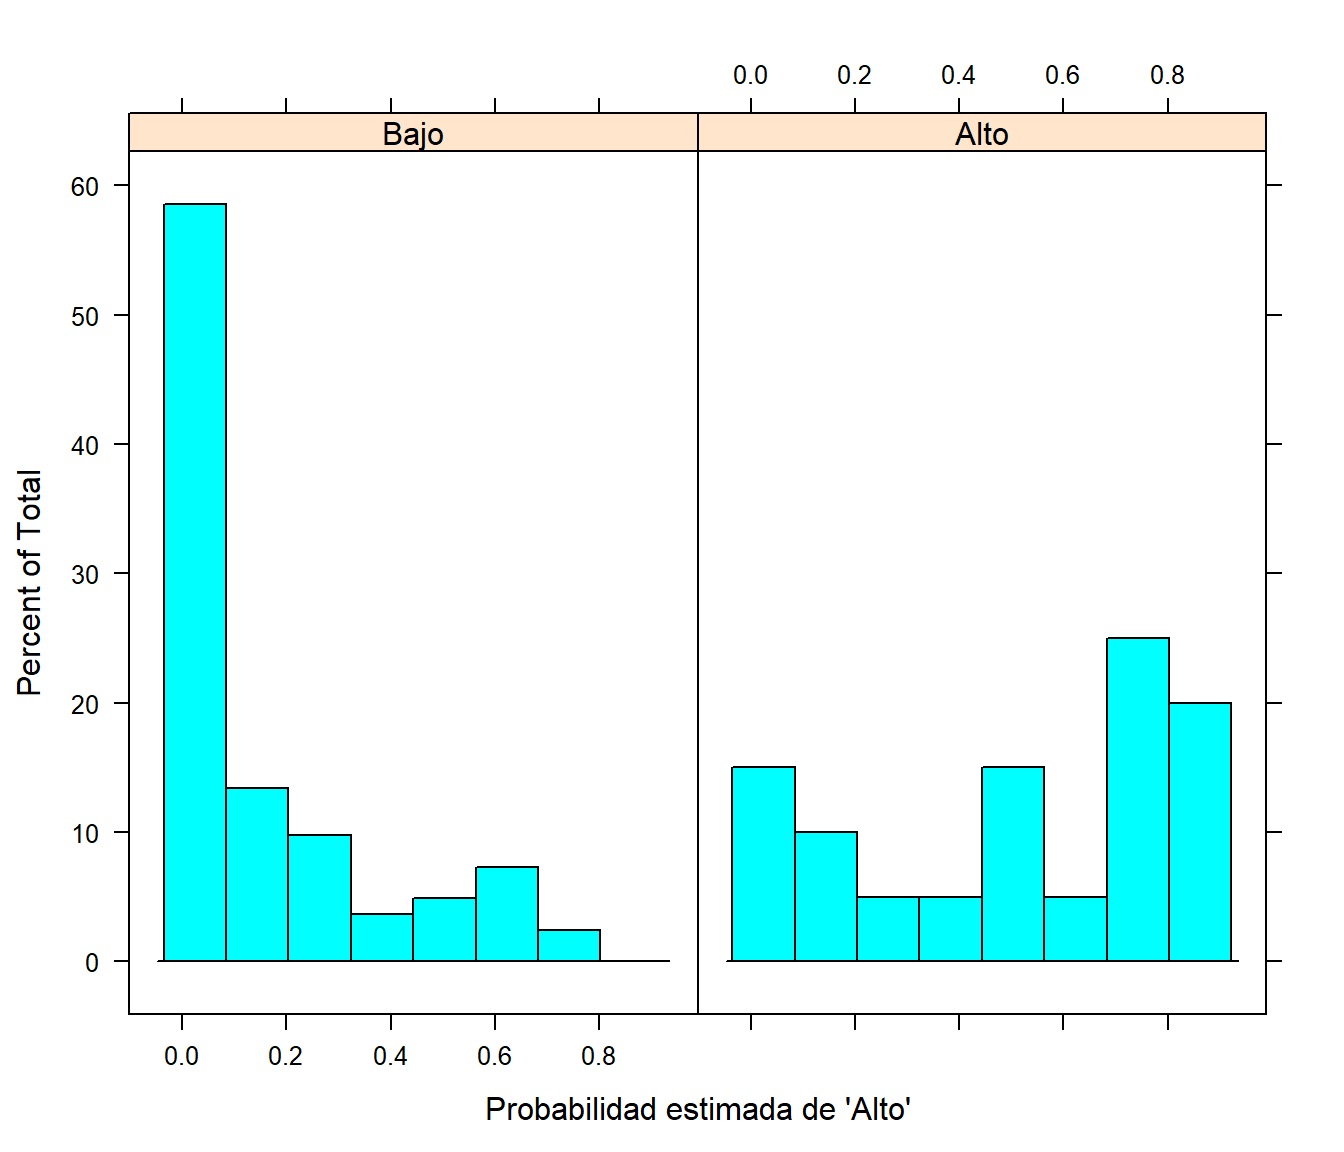
\includegraphics[width=0.8\linewidth]{01-introduccion_files/figure-latex/unnamed-chunk-19-1} \end{center}

Para evaluar las estimaciones de las probabilidades se suele emplear la
curva ROC (\emph{receiver operating characteristics}, característica
operativa del receptor; diseñada inicialmente en el campo de la
detección de señales). Como ya se comentó, normalmente se emplea
\(c = 0.5\) como punto de corte para clasificar en la categoría de
interés (es lo que se conoce como \emph{regla de Bayes}), aunque se
podrían considerar otros valores (por ejemplo para mejorar la
clasificación en una de las categorías, a costa de empeorar la precisión
global). En la curva ROC se representa la sensibilidad (TPR) frente a la
tasa de falsos negativos (FNR = 1 - TNR = 1 - especificidad) para
distintos valores de corte. Para ello se puede emplear el paquete
\texttt{pROC}:

\begin{Shaded}
\begin{Highlighting}[]
\KeywordTok{library}\NormalTok{(pROC)}
\NormalTok{roc_glm <-}\StringTok{ }\KeywordTok{roc}\NormalTok{(}\DataTypeTok{response =}\NormalTok{ obs, }\DataTypeTok{predictor =}\NormalTok{ p.est)}
\CommentTok{# View((as.data.frame(roc_glm[2:4])))}
\KeywordTok{plot}\NormalTok{(roc_glm)}
\end{Highlighting}
\end{Shaded}

\begin{figure}[!htb]

{\centering 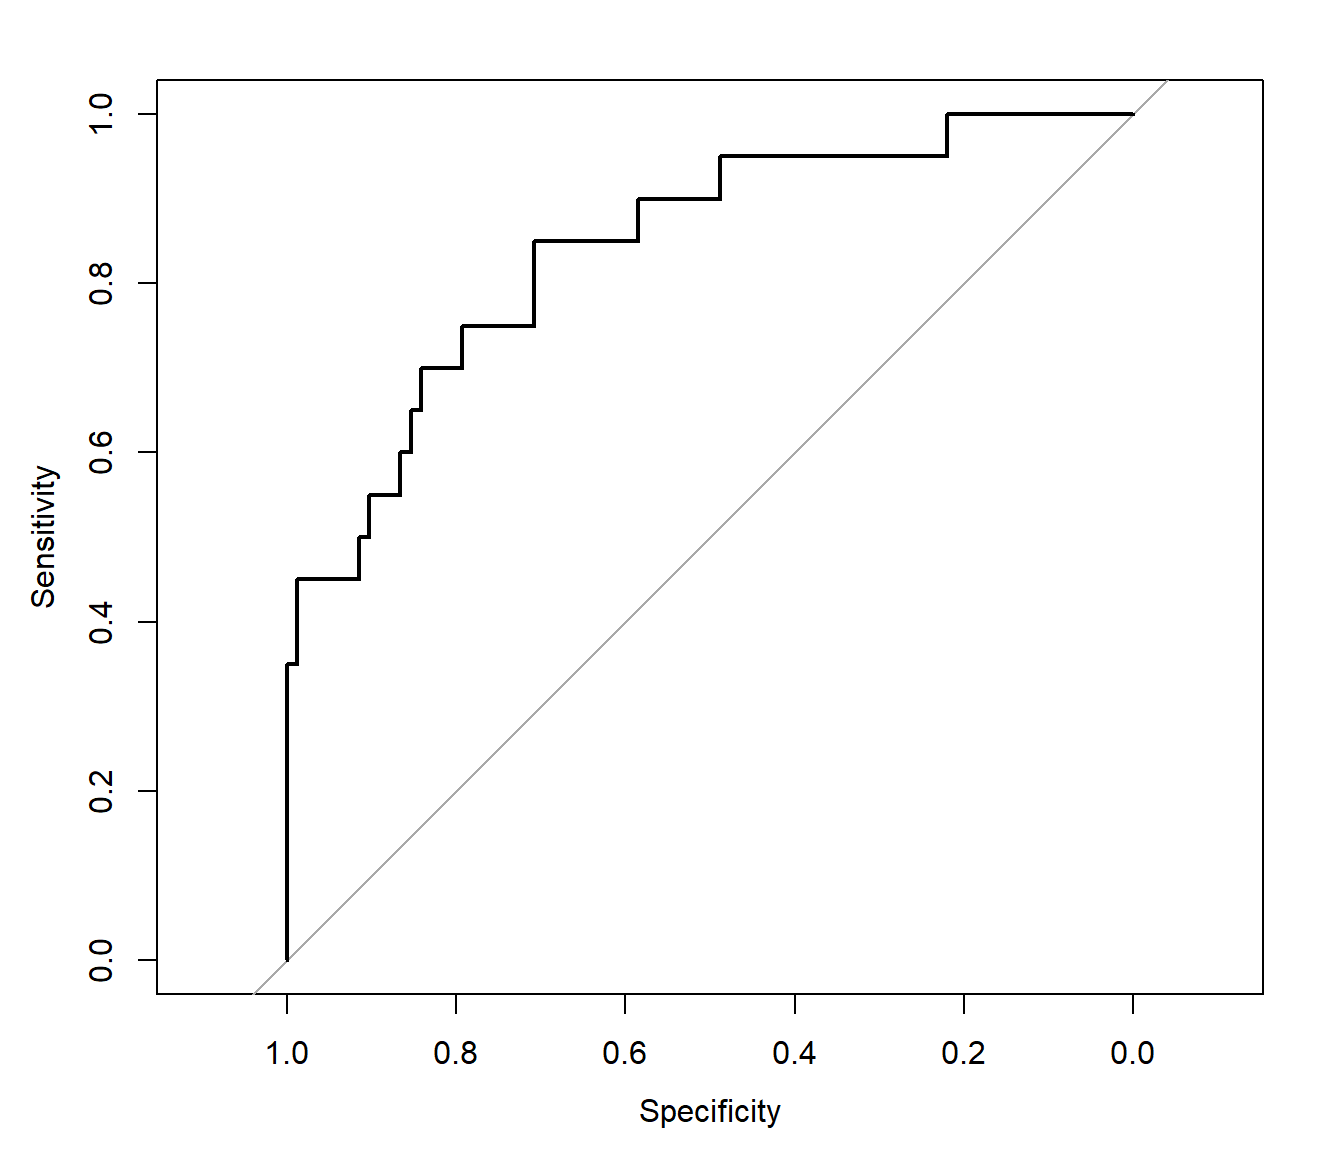
\includegraphics[width=0.8\linewidth]{01-introduccion_files/figure-latex/ROC-curve-1} 

}

\caption{Curva ROC correspondiente al modelo de regresión logística.}\label{fig:ROC-curve}
\end{figure}

\begin{Shaded}
\begin{Highlighting}[]
\CommentTok{# plot(roc_glm, legacy.axes = TRUE)}
\end{Highlighting}
\end{Shaded}

Lo ideal sería que la curva se aproximase a la esquina superior
izquierda (máxima sensibilidad y especificidad). La recta diagonal se
correspondería con un clasificador aleatorio. Una medida global del
rendimiento del clasificador es el área bajo la curva ROC (AUC;
equivalente al estadístico U de Mann-Whitney o al índice de Gini). Un
clasificador perfecto tendría un valor de 1 y 0.5 uno aleatorio.

\begin{Shaded}
\begin{Highlighting}[]
\CommentTok{# roc_glm$auc}
\NormalTok{roc_glm}
\end{Highlighting}
\end{Shaded}

\begin{verbatim}
## 
## Call:
## roc.default(response = obs, predictor = p.est)
## 
## Data: p.est in 82 controls (obs Bajo) < 20 cases (obs Alto).
## Area under the curve: 0.8427
\end{verbatim}

\begin{Shaded}
\begin{Highlighting}[]
\KeywordTok{ci.auc}\NormalTok{(roc_glm)}
\end{Highlighting}
\end{Shaded}

\begin{verbatim}
## 95% CI: 0.7428-0.9426 (DeLong)
\end{verbatim}

Como comentario adicional, aunque se puede modificar el punto de corte
para mejorar la clasificación en la categoría de interés (de hecho,
algunas herramientas como \texttt{h2o} lo modifican por defecto; en este
caso concreto para maximizar \(F_1\) en la muestra de entrenamiento),
muchos métodos de clasificación (como los basados en árboles descritos
en el Capítulo 2) admiten como opción una matriz de pérdidas que se
tendrá en cuenta para medir la eficiencia durante el aprendizaje y
normalmente esta sería la aproximación recomendada.

En el caso de más de dos categorías podríamos generar una matriz de
confusión de forma análoga, aunque en este caso en principio solo
podríamos calcular medidas globales de la precisión como la tasa de
aciertos o el coeficiente kappa de Cohen. Podríamos obtener también
medidas por clase, como la sensibilidad y la especificidad, siguiendo la
estrategia ``uno contra todos'' descrita en la Sección \ref{notacion}.
Esta aproximación es la que sigue la función \texttt{confusionMatrix()}
del paquete \texttt{caret} (devuelve las medidas comparando cada
categoría con las restantes en el componente \texttt{\$byClass}).

Como ejemplo ilustrativo consideraremos el conocido conjunto de datos
\texttt{iris} (Fisher, 1936) en el que el objetivo es clasificar flores
de lirio en tres especies (\texttt{Species}) a partir del largo y ancho
de sépalos y pétalos, aunque en este caso emplearemos un clasificador
aleatorio.

\begin{Shaded}
\begin{Highlighting}[]
\KeywordTok{data}\NormalTok{(iris)}
\CommentTok{# Partición de los datos}
\NormalTok{datos <-}\StringTok{ }\NormalTok{iris}
\KeywordTok{set.seed}\NormalTok{(}\DecValTok{1}\NormalTok{)}
\NormalTok{nobs <-}\StringTok{ }\KeywordTok{nrow}\NormalTok{(datos)}
\NormalTok{itrain <-}\StringTok{ }\KeywordTok{sample}\NormalTok{(nobs, }\FloatTok{0.8} \OperatorTok{*}\StringTok{ }\NormalTok{nobs)}
\NormalTok{train <-}\StringTok{ }\NormalTok{datos[itrain, ]}
\NormalTok{test <-}\StringTok{ }\NormalTok{datos[}\OperatorTok{-}\NormalTok{itrain, ]}
\CommentTok{# Entrenamiento }
\NormalTok{prevalences <-}\StringTok{ }\KeywordTok{table}\NormalTok{(train}\OperatorTok{$}\NormalTok{Species)}\OperatorTok{/}\KeywordTok{nrow}\NormalTok{(train)}
\NormalTok{prevalences}
\end{Highlighting}
\end{Shaded}

\begin{verbatim}
## 
##     setosa versicolor  virginica 
##  0.3250000  0.3166667  0.3583333
\end{verbatim}

\begin{Shaded}
\begin{Highlighting}[]
\CommentTok{# Calculo de las predicciones}
\NormalTok{levels <-}\StringTok{ }\KeywordTok{names}\NormalTok{(prevalences) }\CommentTok{# levels(train$Species)}
\NormalTok{f <-}\StringTok{ }\KeywordTok{factor}\NormalTok{(levels, }\DataTypeTok{levels =}\NormalTok{ levels) }\CommentTok{# factor(levels) valdría en este caso al estar por orden alfabético}
\NormalTok{pred.rand <-}\StringTok{ }\KeywordTok{sample}\NormalTok{(f, }\KeywordTok{nrow}\NormalTok{(test), }\DataTypeTok{replace =} \OtherTok{TRUE}\NormalTok{, }\DataTypeTok{prob =}\NormalTok{ prevalences)}
\CommentTok{# Evaluación}
\NormalTok{caret}\OperatorTok{::}\KeywordTok{confusionMatrix}\NormalTok{(pred.rand, test}\OperatorTok{$}\NormalTok{Species)}
\end{Highlighting}
\end{Shaded}

\begin{verbatim}
## Confusion Matrix and Statistics
## 
##             Reference
## Prediction   setosa versicolor virginica
##   setosa          3          3         1
##   versicolor      4          2         5
##   virginica       4          7         1
## 
## Overall Statistics
##                                           
##                Accuracy : 0.2             
##                  95% CI : (0.0771, 0.3857)
##     No Information Rate : 0.4             
##     P-Value [Acc > NIR] : 0.9943          
##                                           
##                   Kappa : -0.1862         
##                                           
##  Mcnemar's Test P-Value : 0.5171          
## 
## Statistics by Class:
## 
##                      Class: setosa Class: versicolor Class: virginica
## Sensitivity                 0.2727           0.16667          0.14286
## Specificity                 0.7895           0.50000          0.52174
## Pos Pred Value              0.4286           0.18182          0.08333
## Neg Pred Value              0.6522           0.47368          0.66667
## Prevalence                  0.3667           0.40000          0.23333
## Detection Rate              0.1000           0.06667          0.03333
## Detection Prevalence        0.2333           0.36667          0.40000
## Balanced Accuracy           0.5311           0.33333          0.33230
\end{verbatim}

\section{La maldición de la
dimensionalidad}\label{la-maldiciuxf3n-de-la-dimensionalidad}

Podríamos pensar que al aumentar el número de variables explicativas se
mejora la capacidad predictiva de los modelos. Lo cual, en general,
sería cierto si realmente los predictores fuesen de utilidad para
explicar la respuesta. Sin embargo, al aumentar el número de dimensiones
se pueden agravar notablemente muchos de los problemas que ya pueden
aparecer en dimensiones menores, esto es lo que se conoce como la
\emph{maldición de la dimensionalidad} (\emph{curse of dimensionality},
Bellman, 1961).

Uno de estos problemas es el denominado \emph{efecto frontera} que ya
puede aparecer en una dimensión, especialmente al trabajar con modelos
flexibles (como ajustes polinómicos con grados altos o los métodos
locales que trataremos en el Capítulo 6). La idea es que en la
``frontera'' del rango de valores de una variable explicativa vamos a
disponer de pocos datos y los errores de predicción van a tener gran
variabilidad (se están haciendo extrapolaciones de los datos, más que
interpolaciones, y van a ser menos fiables).

Como ejemplo consideraremos un problema de regresión simple, con un
conjunto de datos simulados (del proceso ya considerado en la Sección
\ref{bias-variance}) con 100 observaciones (que ya podríamos considerar
que no es muy pequeño).

\begin{Shaded}
\begin{Highlighting}[]
\CommentTok{# Simulación datos}
\NormalTok{n <-}\StringTok{ }\DecValTok{100}
\NormalTok{x <-}\StringTok{ }\KeywordTok{seq}\NormalTok{(}\DecValTok{0}\NormalTok{, }\DecValTok{1}\NormalTok{, }\DataTypeTok{length =}\NormalTok{ n)}
\NormalTok{mu <-}\StringTok{ }\DecValTok{2} \OperatorTok{+}\StringTok{ }\DecValTok{4}\OperatorTok{*}\NormalTok{(}\DecValTok{5}\OperatorTok{*}\NormalTok{x }\OperatorTok{-}\StringTok{ }\DecValTok{1}\NormalTok{)}\OperatorTok{*}\NormalTok{(}\DecValTok{4}\OperatorTok{*}\NormalTok{x }\OperatorTok{-}\StringTok{ }\DecValTok{2}\NormalTok{)}\OperatorTok{*}\NormalTok{(x }\OperatorTok{-}\StringTok{ }\FloatTok{0.8}\NormalTok{)}\OperatorTok{^}\DecValTok{2} \CommentTok{# grado 4}
\NormalTok{sd <-}\StringTok{ }\FloatTok{0.5}
\KeywordTok{set.seed}\NormalTok{(}\DecValTok{1}\NormalTok{)}
\NormalTok{y <-}\StringTok{ }\NormalTok{mu }\OperatorTok{+}\StringTok{ }\KeywordTok{rnorm}\NormalTok{(n, }\DecValTok{0}\NormalTok{, sd)}
\NormalTok{datos <-}\StringTok{ }\KeywordTok{data.frame}\NormalTok{(}\DataTypeTok{x =}\NormalTok{ x, }\DataTypeTok{y =}\NormalTok{ y)}
\KeywordTok{plot}\NormalTok{(x, y) }
\KeywordTok{lines}\NormalTok{(x, mu, }\DataTypeTok{lwd =} \DecValTok{2}\NormalTok{, }\DataTypeTok{col =} \StringTok{"lightgray"}\NormalTok{)}
\end{Highlighting}
\end{Shaded}

\begin{figure}[!htb]

{\centering 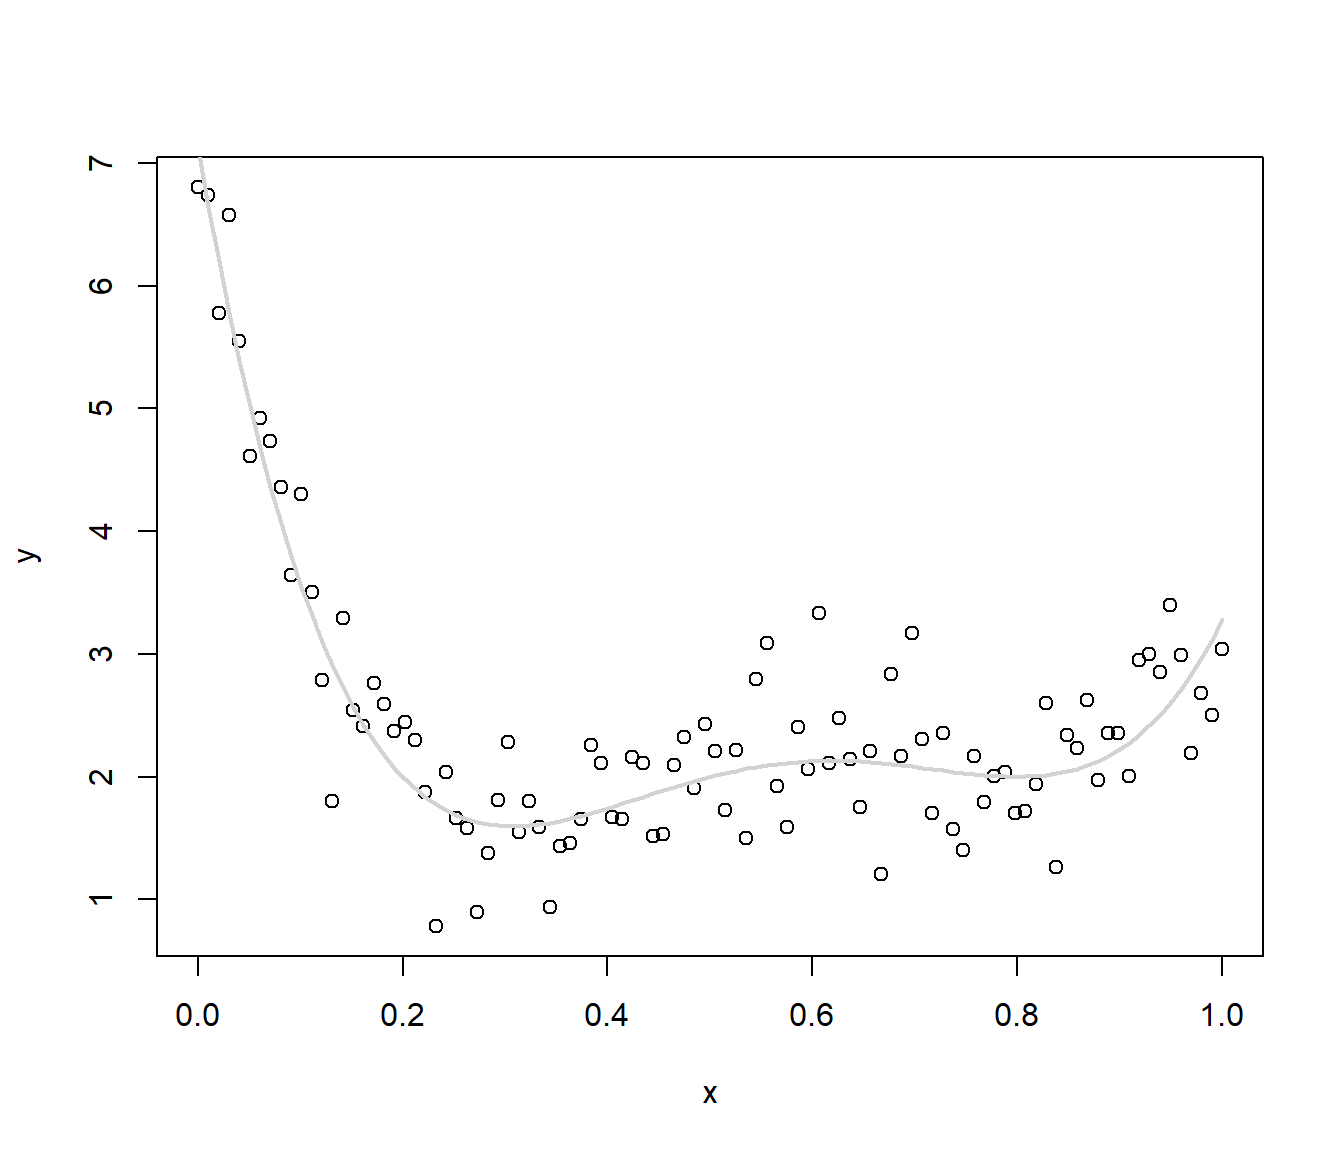
\includegraphics[width=0.8\linewidth]{01-introduccion_files/figure-latex/simdat100-1} 

}

\caption{Muestra simulada y tendencia teórica.}\label{fig:simdat100}
\end{figure}

Cuando el número de datos es más o menos grande podríamos pensar en
predecir la respuesta a partir de lo que ocurre en las observaciones
cercanas a la posición de predicción, esta es la idea de los métodos
locales (Capítulo 6). Uno de los métodos de este tipo más conocidos es
el de los \emph{k-vecinos más cercanos} (\emph{k-nearest neighbors};
KNN). Se trata de un método muy simple, pero que puede ser muy efectivo,
que se basa en la idea de que localmente la media condicional (la
predicción óptima) es constante. Concretamente, dados un entero \(k\)
(hiperparámetro) y un conjunto de entrenamiento \(\mathcal{T}\), para
obtener la predicción correspondiente a un vector de valores de las
variables explicativas \(\mathbf{x}\), el método de regresión\footnote{En
  el caso de clasificación se considerarían las variables indicadoras de
  las categorías y se obtendrían las frecuencias relativas en el
  vecindario como estimaciones de las probabilidades de las clases.} KNN
promedia las obsevaciones en un vecindario
\(\mathcal{N}_k(\mathbf{x}, \mathcal{T})\) formado por las \(k\)
observaciones más cercanas a \(\mathbf{x}\):
\[\hat{Y}(\mathbf{x}) = \hat{m}(\mathbf{x}) = \frac{1}{k} \sum_{i \in \mathcal{N}_k(\mathbf{x}, \mathcal{T})} Y_i\]
(sería necesario definir una distancia, normalmente la distancia
euclídea de los predictores estandarizados).

Este método está implementado en numerosos paquetes, por ejemplo en la
función \texttt{knnreg()} del paquete \texttt{caret}:

\begin{Shaded}
\begin{Highlighting}[]
\KeywordTok{library}\NormalTok{(caret)}

\CommentTok{# Ajuste de los modelos}
\NormalTok{fit1 <-}\StringTok{ }\KeywordTok{knnreg}\NormalTok{(y }\OperatorTok{~}\StringTok{ }\NormalTok{x, }\DataTypeTok{data =}\NormalTok{ datos, }\DataTypeTok{k =} \DecValTok{5}\NormalTok{) }\CommentTok{# 5 observaciones más cercanas (5% de los datos)}
\NormalTok{fit2 <-}\StringTok{ }\KeywordTok{knnreg}\NormalTok{(y }\OperatorTok{~}\StringTok{ }\NormalTok{x, }\DataTypeTok{data =}\NormalTok{ datos, }\DataTypeTok{k =} \DecValTok{10}\NormalTok{)}
\NormalTok{fit3 <-}\StringTok{ }\KeywordTok{knnreg}\NormalTok{(y }\OperatorTok{~}\StringTok{ }\NormalTok{x, }\DataTypeTok{data =}\NormalTok{ datos, }\DataTypeTok{k =} \DecValTok{20}\NormalTok{)}

\KeywordTok{plot}\NormalTok{(x, y) }
\KeywordTok{lines}\NormalTok{(x, mu, }\DataTypeTok{lwd =} \DecValTok{2}\NormalTok{, }\DataTypeTok{col =} \StringTok{"lightgray"}\NormalTok{)}
\NormalTok{newdata <-}\StringTok{ }\KeywordTok{data.frame}\NormalTok{(}\DataTypeTok{x =}\NormalTok{ x)}
\KeywordTok{lines}\NormalTok{(x, }\KeywordTok{predict}\NormalTok{(fit1, newdata), }\DataTypeTok{lwd =} \DecValTok{2}\NormalTok{, }\DataTypeTok{lty =} \DecValTok{3}\NormalTok{)}
\KeywordTok{lines}\NormalTok{(x, }\KeywordTok{predict}\NormalTok{(fit2, newdata), }\DataTypeTok{lwd =} \DecValTok{2}\NormalTok{, }\DataTypeTok{lty =} \DecValTok{2}\NormalTok{)}
\KeywordTok{lines}\NormalTok{(x, }\KeywordTok{predict}\NormalTok{(fit3, newdata), }\DataTypeTok{lwd =} \DecValTok{2}\NormalTok{)}
\KeywordTok{legend}\NormalTok{(}\StringTok{"topright"}\NormalTok{, }\DataTypeTok{legend =} \KeywordTok{c}\NormalTok{(}\StringTok{"Verdadero"}\NormalTok{, }\StringTok{"5-NN"}\NormalTok{, }\StringTok{"10-NN"}\NormalTok{, }\StringTok{"20-NN"}\NormalTok{), }
       \DataTypeTok{lty =} \KeywordTok{c}\NormalTok{(}\DecValTok{1}\NormalTok{, }\DecValTok{3}\NormalTok{, }\DecValTok{2}\NormalTok{, }\DecValTok{1}\NormalTok{), }\DataTypeTok{lwd =} \DecValTok{2}\NormalTok{, }\DataTypeTok{col =} \KeywordTok{c}\NormalTok{(}\StringTok{"lightgray"}\NormalTok{, }\DecValTok{1}\NormalTok{, }\DecValTok{1}\NormalTok{, }\DecValTok{1}\NormalTok{))}
\end{Highlighting}
\end{Shaded}

\begin{figure}[!htb]

{\centering 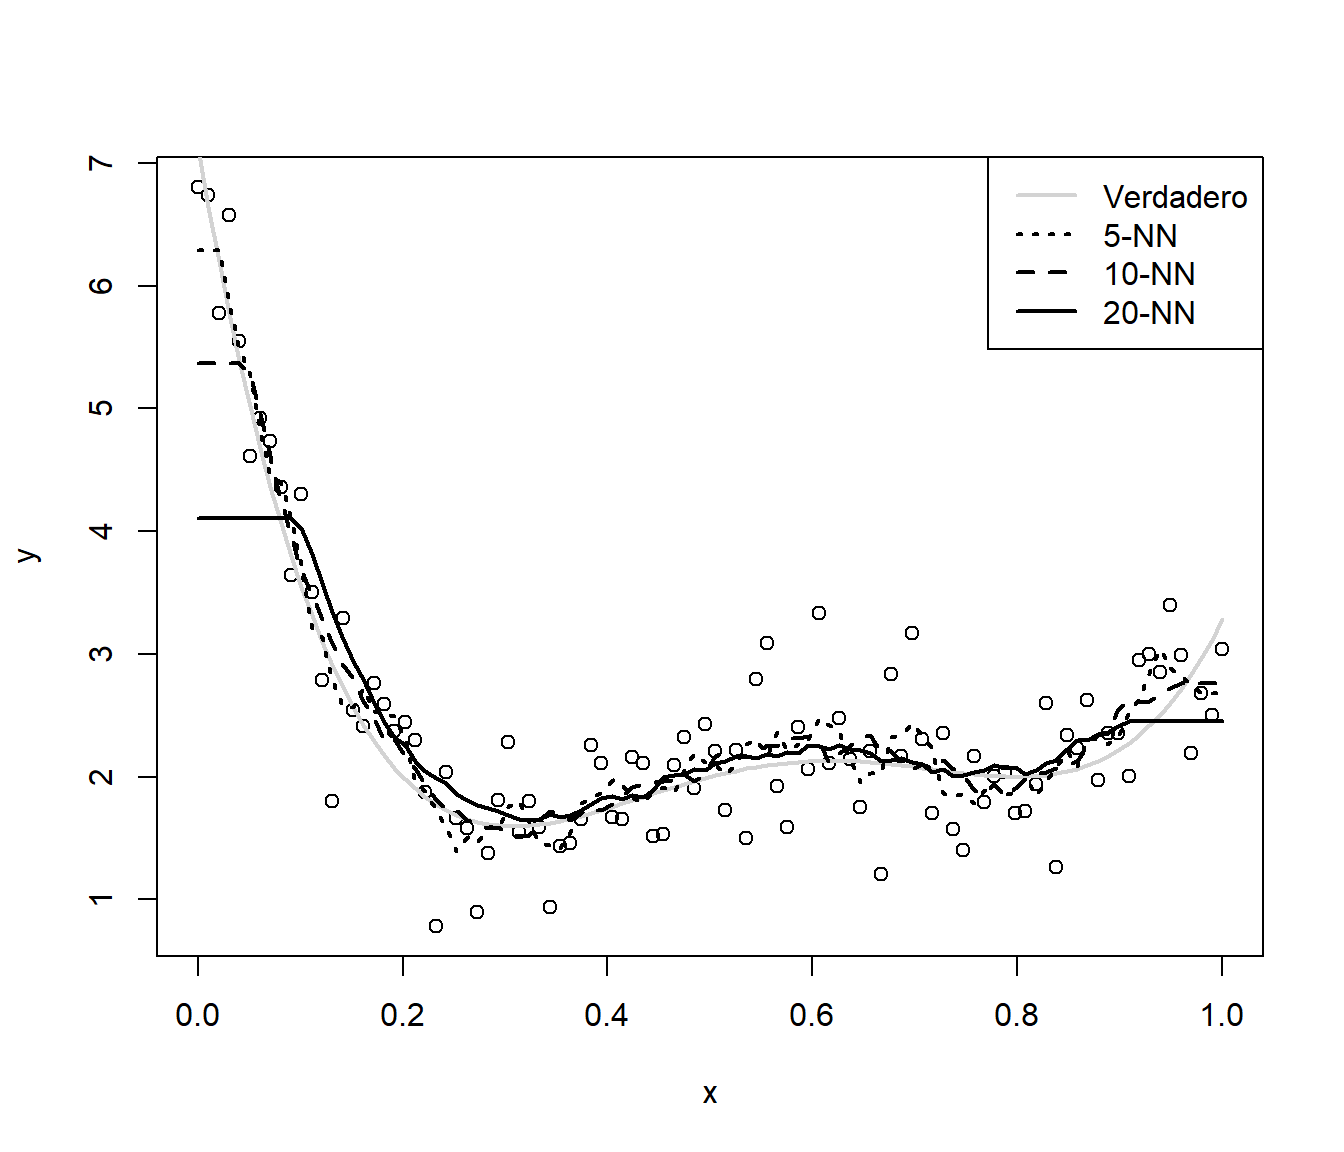
\includegraphics[width=0.8\linewidth]{01-introduccion_files/figure-latex/knnfit2-1} 

}

\caption{Predicciones con el método KNN y distintos vecindarios}\label{fig:knnfit2}
\end{figure}

A medida que aumenta \(k\) disminuye la complejidad del modelo y se
observa un incremento del efecto frontera. Habría que seleccionar un
valor óptimo de \(k\) (buscando un equilibro entre sesgo y varianza,
como se mostró en la Sección \ref{bias-variance} y se ilustrará en la
última sección de este capítulo empleando este método con el paquete
\texttt{caret}), que dependerá de la tendencia teórica y del número de
datos. En este caso, para \(k=5\), podríamos pensar que el efecto
frontera aparece en el 10\% más externo del rango de la variable
explicativa (con un número mayor de datos podría bajar al 1\%). Al
aumentar el número de variables explicativas, considerando que el 10\%
más externo del rango de cada una de ellas constituye la ``frontera'' de
los datos, tendríamos que la proporción de frontera sería \(1-0.9^d\),
siendo \(d\) el número de dimensiones. Lo que se traduce que con
\(d = 10\) el 65\% del espacio predictivo sería frontera y en torno al
88\% para \(d=20\), es decir, al aumentar el número de dimensiones el
problema del efecto frontera será generalizado.

\begin{Shaded}
\begin{Highlighting}[]
\KeywordTok{curve}\NormalTok{(}\DecValTok{1} \OperatorTok{-}\StringTok{ }\FloatTok{0.9}\OperatorTok{^}\NormalTok{x, }\DecValTok{0}\NormalTok{, }\DecValTok{200}\NormalTok{, }\DataTypeTok{ylab =} \StringTok{'Proporción de "frontera"'}\NormalTok{, }\DataTypeTok{xlab =} \StringTok{'Número de dimensiones'}\NormalTok{)}
\KeywordTok{curve}\NormalTok{(}\DecValTok{1} \OperatorTok{-}\StringTok{ }\FloatTok{0.95}\OperatorTok{^}\NormalTok{x, }\DataTypeTok{lty =} \DecValTok{2}\NormalTok{, }\DataTypeTok{add =} \OtherTok{TRUE}\NormalTok{)}
\KeywordTok{curve}\NormalTok{(}\DecValTok{1} \OperatorTok{-}\StringTok{ }\FloatTok{0.99}\OperatorTok{^}\NormalTok{x, }\DataTypeTok{lty =} \DecValTok{3}\NormalTok{, }\DataTypeTok{add =} \OtherTok{TRUE}\NormalTok{)}
\KeywordTok{abline}\NormalTok{(}\DataTypeTok{h =} \FloatTok{0.5}\NormalTok{, }\DataTypeTok{col =} \StringTok{"lightgray"}\NormalTok{)}
\KeywordTok{legend}\NormalTok{(}\StringTok{"bottomright"}\NormalTok{, }\DataTypeTok{title =} \StringTok{"Rango en cada dimensión", legend = c("}\DecValTok{10}\OperatorTok\StringTok{", "}\DecValTok{1}\NormalTok{%}\StringTok{"), }
\StringTok{       lty = c(1, 2, 3))}
\end{Highlighting}
\end{Shaded}

\begin{center}\includegraphics[width=0.8\linewidth]{01-introduccion_files/figure-latex/unnamed-chunk-22-1} \end{center}

Desde otro punto de vista, suponiendo que los predictores se distribuyen
de forma uniforme, la densidad de las observaciones es proporcional a
\(n^{1/d}\), siendo \(n\) el tamaño muestral. Por lo que si consideramos
que una muestra de tamaño \(n=100\) es suficientemente densa en una
dimensión, para obtener la misma densidad muestral en 10 dimensiones
tendríamos que disponer de un tamaño muestral de
\(n = 100^{10} = 10^{20}\). Por tanto, cuando el número de dimensiones
es grande no va a haber muchas observaciones en el entorno de la
posición de predicción y puede haber serios problemas de sobreajuste si
se pretende emplear un modelo demasiado flexible (por ejemplo KNN con
\(k\) pequeño). Hay que tener en cuenta que, en general, fijado el
tamaño muestral, la flexibilidad de los modelos aumenta al aumentar el
número de dimensiones del espacio predictivo.

Para concluir, otro de los problemas que se agravan notablemente al
aumentar el número de dimensiones es el de colinealidad (o concurvidad)
que puede producir que muchos métodos (como los modelos lineales o las
redes neuronales) sean muy poco eficientes o inestables (llegando
incluso a que no se puedan aplicar), además de que complica notablemente
la interpretación de cualquier método. Esto está relacionado también con
la dificultad para determinar que variables son de interés para predecir
la respuesta (i.e.~no son ruido). Debido a la aleatoriedad, predictores
que realmente no están relacionados con la respuesta pueden ser tenidos
en cuenta por el modelo con mayor facilidad (KNN con las opciones
habituales tiene en cuenta todos los predictores con el mismo peso). Lo
que resulta claro es que si se agrega ruido se producirá un incremento
en el error de predicción. Incluso si las variables añadidas resultan de
interés, si el número de observaciones es pequeño en comparación, el
incremento en la variabilidad de las predicciones puede no compensar la
disminución del sesgo de predicción.

Como conclusión, en el caso multidimensional habrá que tratar de emplear
métodos que minimicen estos problemas.

\section{Análisis e interpretación de los
modelos}\label{anuxe1lisis-e-interpretaciuxf3n-de-los-modelos}

El análisis e interpretación de modelos es un campo muy activo en AE/ML,
para el que recientemente se ha acuñado el término de
\emph{interpretable machine learning} (IML). A continuación se resumen
brevemente algunas de las principales ideas, para más detalles ver por
ejemplo \href{https://christophm.github.io/interpretable-ml-book}{Molnar
(2020)}.

Como ya se comentó, a medida que aumenta la complejidad de los modelos
generalmente disminuye su interpretabilidad, por lo que normalmente
interesa encontrar el modelo más simple posible que resulte de utilidad
para los objetivos propuestos. Aunque el principal objetivo sea la
predicción, una vez obtenido el modelo final suele interesar medir la
importancia de cada predictor en el modelo y si es posible como influyen
en la predicción de la respuesta, es decir, estudiar el efecto de las
variables explicativas. Esto puede presentar serias dificultades
especialmente en modelos complejos en los que hay interacciones entre
los predictores (el efecto de una variable explicativa depende de los
valores de otras).

La mayoría de los métodos de aprendizaje supervisado permiten obtener
medidas de la importancia de las variables explicativas en la predicción
(ver p.e. la
\href{https://topepo.github.io/caret/variable-importance.html}{ayuda} de
la función \texttt{caret::varImp()}; algunos, como los basados en
árboles, incluso de las no incluidas en el modelo final). Muchos de los
métodos de clasificación, en lugar de proporcionar medidas globales,
calculan medidas para cada categoría. Alternativamente también se pueden
obtener medidas de la importancia de las variables mediante
procedimientos generales (en el sentido de que se pueden aplicar a
cualquier modelo), pero suelen requerir de mucho más tiempo de
computación (ver p.e.
\href{https://christophm.github.io/interpretable-ml-book}{Molnar, 2020},
\href{https://christophm.github.io/interpretable-ml-book/agnostic.htm}{Capítulo
5}).

En algunos de los métodos se modela explícitamente los efectos de los
distintos predictores y estos se pueden analizar con (mas o menos)
facilidad. Hay que tener en cuenta que, al margen de las interacciones,
la colinealidad/concurvidad dificulta notablemente el estudio de los
efectos de las variables explicativas. Otros métodos son más del tipo
``caja negra'' (\emph{black box}) y precisan de aproximaciones más
generales, como los gráficos PDP (\emph{Partial Dependence Plots};
Friedman y Popescu, 2008; ver también
\href{https://journal.r-project.org/archive/2017/RJ-2017-016/index.html}{Greenwell,
2017}) o las curvas ICE (\emph{Individual Conditional Expectation};
\href{https://doi.org/10.1080/10618600.2014.907095}{Goldstein \emph{et
al.} , 2015}). Estos métodos\footnote{Similares a los gráficos parciales
  de residuos de los modelos lineales o aditivos (ver p.e. las funciones
  \texttt{termplot()}, \texttt{car::crPlots()} o
  \texttt{car::avPlots()}).} tratan de estimar el efecto marginal de las
variables explicativas, es decir, la variación en la predicción a medida
que varía una variable explicativa manteniendo constantes el resto. La
principal diferencia entre ambas aproximaciones es que los gráficos PDP
muestran una única curva con el promedio de la respuesta mientras que
las curvas ICE muestran una curva para cada observación (para más
detalles ver las referencias anteriores).

En problemas de clasificación también se están empleando la teoría de
juegos cooperativos y las técnicas de optimización de Investigación
Operativa para evaluar la importancia de las variables predictoras y
determinar las más influyentes. Por citar algunos, Strumbelj y Kononenko
(2010) propusieron un procedimiento general basado en el valor de
Shapley de juegos cooperativos, y en Agor y Özaltın (2019) se propone el
uso de algoritmos genéticos para determinar los predictores más
influyentes.

Paquetes y funciones de R:

\begin{itemize}
\item
  \href{https://bgreenwell.github.io/pdp/index.html}{\texttt{pdp}}:
  Partial Dependence Plots

  (también implementa curvas ICE y es compatible con \texttt{caret})
\item
  \href{https://christophm.github.io/iml}{\texttt{iml}}: Interpretable
  Machine Learning
\item
  \href{https://modeloriented.github.io/DALEX}{\texttt{DALEX}}: moDel
  Agnostic Language for Exploration and eXplanation
\item
  \href{https://lime.data-imaginist.com}{\texttt{lime}}: Local
  Interpretable Model-Agnostic Explanations
\item
  \href{https://koalaverse.github.io/vip/index.html}{\texttt{vip}}:
  Variable Importance Plots
\item
  \texttt{caret::varImp()}, \texttt{h2o::h2o.partialPplot()}\ldots{}
\end{itemize}

En los siguientes capítulos se mostrarán ejemplos empleando algunas de
estas herramientas.

\section{\texorpdfstring{Introducción al paquete
\texttt{caret}}{Introducción al paquete caret}}\label{caret}

Como ya se comentó en la Sección \ref{metodos-pkgs}, el paquete
\texttt{caret} (abreviatura de \emph{Classification And REgression
Training}) proporciona una interfaz unificada que simplifica el proceso
de modelado empleando la mayoría de los métodos de AE implementados en R
(actualmente admite 238 métodos; ver el
\href{https://topepo.github.io/caret/available-models.html}{Capítulo 6}
del \href{https://topepo.github.io/caret}{manual} de este paquete).
Además de proporcionar rutinas para los principales pasos del proceso,
incluye también numerosas funciones auxiliares que permitirían
implementar nuevos procedimientos.

Enlaces:

\begin{itemize}
\item
  \href{https://topepo.github.io/caret}{Manual}

  \begin{itemize}
  \item
    \href{https://topepo.github.io/caret/pre-processing.html}{3.
    Pre-Processing}
  \item
    \href{https://topepo.github.io/caret/model-training-and-tuning.html}{5.
    Model Training and Tuning}
  \item
    \href{https://topepo.github.io/caret/available-models.html}{6.
    Available Models}
  \item
    \href{https://topepo.github.io/caret/measuring-performance.html}{17.
    Measuring Performance}
  \end{itemize}
\item
  \href{https://cran.r-project.org/web/packages/caret/vignettes/caret.html}{Vignette}
\item
  \href{https://raw.githubusercontent.com/rstudio/cheatsheets/master/caret.pdf}{Cheat
  Sheet}
\end{itemize}

La función principal es \texttt{train()} (descrita más adelante), que
incluye un parámetro \texttt{method} que permite establecer el modelo
mediante una cadena de texto. Podemos obtener información sobre los
modelos disponibles con las funciones \texttt{getModelInfo()} y
\texttt{modelLookup()} (puede haber varias implementaciones del mismo
método con distintas configuraciones de hiperparámetros; también se
pueden definir nuevos modelos, ver el
\href{https://topepo.github.io/caret/using-your-own-model-in-train.html}{Capítulo
13} del \href{https://topepo.github.io/caret}{manual}).

\begin{Shaded}
\begin{Highlighting}[]
\KeywordTok{library}\NormalTok{(caret)}
\KeywordTok{str}\NormalTok{(}\KeywordTok{names}\NormalTok{(}\KeywordTok{getModelInfo}\NormalTok{())) }\CommentTok{# Listado de todos los métodos disponibles}
\end{Highlighting}
\end{Shaded}

\begin{verbatim}
##  chr [1:238] "ada" "AdaBag" "AdaBoost.M1" "adaboost" "amdai" "ANFIS" ...
\end{verbatim}

\begin{Shaded}
\begin{Highlighting}[]
\CommentTok{# names(getModelInfo("knn", regex = TRUE)) # Por defecto devuelve coincidencias parciales}
\KeywordTok{modelLookup}\NormalTok{(}\StringTok{"knn"}\NormalTok{)  }\CommentTok{# Información sobre hiperparámetros}
\end{Highlighting}
\end{Shaded}

\begin{verbatim}
##   model parameter      label forReg forClass probModel
## 1   knn         k #Neighbors   TRUE     TRUE      TRUE
\end{verbatim}

Este paquete permite, entre otras cosas:

\begin{itemize}
\item
  Partición de los datos

  \begin{itemize}
  \item
    \texttt{createDataPartition(y,\ p\ =\ 0.5,\ list\ =\ TRUE,\ ...)}:
    crea particiones balanceadas de los datos.

    \begin{itemize}
    \item
      En el caso de que la respuesta \texttt{y} sea categórica realiza
      el muestreo en cada clase. Para respuestas numéricas emplea
      cuantiles (definidos por el argumento
      \texttt{groups\ =\ min(5,\ length(y))}).
    \item
      \texttt{p}: proporción de datos en la muestra de entrenamiento.
    \item
      \texttt{list}: lógico; determina si el resultado es una lista con
      las muestras o un vector (o matriz) de índices
    \end{itemize}
  \item
    Funciones auxiliares: \texttt{createFolds()},
    \texttt{createMultiFolds()}, \texttt{groupKFold()},
    \texttt{createResample()}, \texttt{createTimeSlices()}
  \end{itemize}
\item
  Análisis descriptivo: \texttt{featurePlot()}
\item
  Preprocesado de los datos:

  \begin{itemize}
  \item
    La función principal es
    \texttt{preProcess(x,\ method\ =\ c("center",\ "scale"),\ ...)},
    aunque se puede integrar en el entrenamiento (función
    \texttt{train()}) para estimar los parámetros de las
    transformaciones a partir de la muestra de entrenamiento y
    posteriormente aplicarlas automáticamente al hacer nuevas
    predicciones (p.e. en la muestra de test).
  \item
    El parámetro \texttt{method} permite establecer una lista de
    procesados:

    \begin{itemize}
    \item
      Imputación: \texttt{"knnImpute"}, \texttt{"bagImpute"} o
      \texttt{"medianImpute"}
    \item
      Creación y transformación de variables explicativas:
      \texttt{"center"}, \texttt{"scale"}, \texttt{"range"},
      \texttt{"BoxCox"}, \texttt{"YeoJohnson"}, \texttt{"expoTrans"},
      \texttt{"spatialSign"}

      Funciones auxiliares: \texttt{dummyVars()}\ldots{}
    \item
      Selección de predictores y extracción de componentes:
      \texttt{"corr"}, \texttt{"nzv"}, \texttt{"zv"},
      \texttt{"conditionalX"}, \texttt{"pca"}, \texttt{"ica"}

      Funciones auxiliares: \texttt{rfe()}\ldots{}
    \end{itemize}
  \end{itemize}
\item
  Entrenamiento y selección de los hiperparámetros del modelo:

  \begin{itemize}
  \item
    La función principal es
    \texttt{train(formula,\ data,\ method\ =\ "rf",\ trControl\ =\ trainControl(),\ tuneGrid\ =\ NULL,\ tuneLength\ =\ 3,\ ...)}

    \begin{itemize}
    \item
      \texttt{trControl}: permite establecer el método de remuestreo
      para la evaluación de los hiperparámetros y el método para
      seleccionar el óptimo, incluyendo las medidas de precisión. Por
      ejemplo
      \texttt{trControl\ =\ trainControl(method\ =\ "cv",\ number\ =\ 10,\ selectionFunction\ =\ "oneSE")}.

      Los métodos disponibles son: \texttt{"boot"}, \texttt{"boot632"},
      \texttt{"optimism\_boot"}, \texttt{"boot\_all"}, \texttt{"cv"},
      \texttt{"repeatedcv"}, \texttt{"LOOCV"}, \texttt{"LGOCV"},
      \texttt{"timeslice"}, \texttt{"adaptive\_cv"},
      \texttt{"adaptive\_boot"} o \texttt{"adaptive\_LGOCV"}
    \item
      \texttt{tuneLength} y \texttt{tuneGrid}: permite establecer
      cuantos hiperparámetros serán evaluados (por defecto 3) o una
      rejilla con las combinaciones de hiperparámetros.
    \item
      \texttt{...} permite establecer opciones específicas de los
      métodos.
    \end{itemize}
  \item
    También admite matrices \texttt{x}, \texttt{y} en lugar de fórmulas
    (o \emph{recetas}: \texttt{recipe()}).
  \item
    Si se imputan datos en el preprocesado será necesario establecer
    \texttt{na.action\ =\ na.pass}.
  \end{itemize}
\item
  Predicción: Una de las ventajas es que incorpora un único método
  \texttt{predict()} para objetos de tipo \texttt{train} con dos únicas
  opciones\footnote{En lugar de la variedad de opciones que emplean los
    distintos paquetes (e.g.: \texttt{type\ =\ "response"},
    \texttt{"class"}, \texttt{"posterior"},
    \texttt{"probability"}\ldots{} ).}
  \texttt{type\ =\ c("raw",\ "prob")}, la primera para obtener
  predicciones de la respuesta y la segunda para obtener estimaciones de
  las probabilidades (en los métodos de clasificación que lo admitan).

  Además, si se incluyo un preprocesado en el entrenamiento, se
  emplearán las mismas transformaciones en un nuevo conjunto de datos
  \texttt{newdata}.
\item
  Evaluación de los modelos

  \begin{itemize}
  \item
    \texttt{postResample(pred,\ obs,\ ...)}: regresión
  \item
    \texttt{confusionMatrix(pred,\ obs,\ ...)}: clasificación

    \begin{itemize}
    \tightlist
    \item
      Funciones auxiliares: \texttt{twoClassSummary()},
      \texttt{prSummary()}\ldots{}
    \end{itemize}
  \end{itemize}
\item
  Analisis de la importancia de los predictores:

  \begin{itemize}
  \tightlist
  \item
    \texttt{varImp()}: interfaz a las medidas específicas de los métodos
    de aprendizaje supervisado
    (\href{https://topepo.github.io/caret/variable-importance.html\#model-specific-metrics}{Sección
    15.1}) o medidas genéricas
    (\href{https://topepo.github.io/caret/variable-importance.html\#model-independent-metrics}{Sección
    15.2}).
  \end{itemize}
\end{itemize}

Ejemplo regresión con KNN:

\begin{Shaded}
\begin{Highlighting}[]
\CommentTok{# caret}
\KeywordTok{data}\NormalTok{(Boston, }\DataTypeTok{package =} \StringTok{"MASS"}\NormalTok{)}

\KeywordTok{library}\NormalTok{(caret)}
\CommentTok{# Partición}
\KeywordTok{set.seed}\NormalTok{(}\DecValTok{1}\NormalTok{)}
\NormalTok{itrain <-}\StringTok{ }\KeywordTok{createDataPartition}\NormalTok{(Boston}\OperatorTok{$}\NormalTok{medv, }\DataTypeTok{p =} \FloatTok{0.8}\NormalTok{, }\DataTypeTok{list =} \OtherTok{FALSE}\NormalTok{)}
\NormalTok{train <-}\StringTok{ }\NormalTok{Boston[itrain, ]}
\NormalTok{test <-}\StringTok{ }\NormalTok{Boston[}\OperatorTok{-}\NormalTok{itrain, ]}
\CommentTok{# Entrenamiento y selección de hiperparámetros}
\KeywordTok{set.seed}\NormalTok{(}\DecValTok{1}\NormalTok{)}
\NormalTok{knn <-}\StringTok{ }\KeywordTok{train}\NormalTok{(medv }\OperatorTok{~}\StringTok{ }\NormalTok{., }\DataTypeTok{data =}\NormalTok{ train,}
             \DataTypeTok{method =} \StringTok{"knn"}\NormalTok{,}
             \DataTypeTok{preProc =} \KeywordTok{c}\NormalTok{(}\StringTok{"center"}\NormalTok{, }\StringTok{"scale"}\NormalTok{),}
             \DataTypeTok{tuneGrid =} \KeywordTok{data.frame}\NormalTok{(}\DataTypeTok{k =} \DecValTok{1}\OperatorTok{:}\DecValTok{10}\NormalTok{),}
             \DataTypeTok{trControl =} \KeywordTok{trainControl}\NormalTok{(}\DataTypeTok{method =} \StringTok{"cv"}\NormalTok{, }\DataTypeTok{number =} \DecValTok{10}\NormalTok{))}
\KeywordTok{plot}\NormalTok{(knn)}
\end{Highlighting}
\end{Shaded}

\begin{center}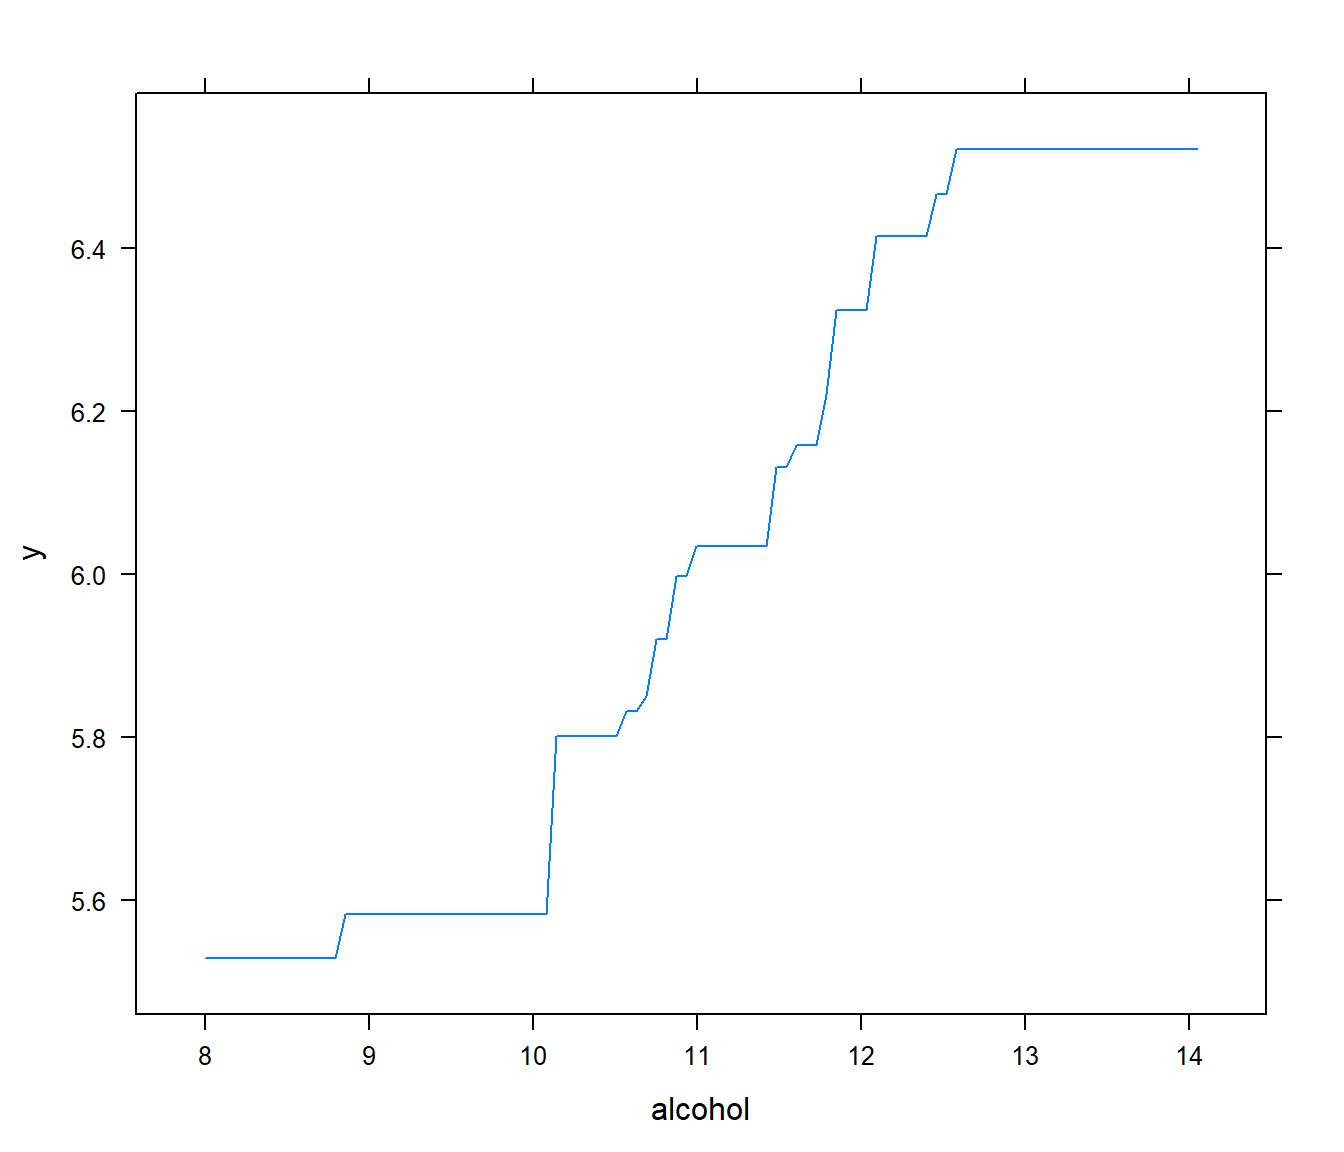
\includegraphics[width=0.8\linewidth]{01-introduccion_files/figure-latex/unnamed-chunk-24-1} \end{center}

\begin{Shaded}
\begin{Highlighting}[]
\KeywordTok{ggplot}\NormalTok{(knn, }\DataTypeTok{highlight =} \OtherTok{TRUE}\NormalTok{)}
\end{Highlighting}
\end{Shaded}

\begin{center}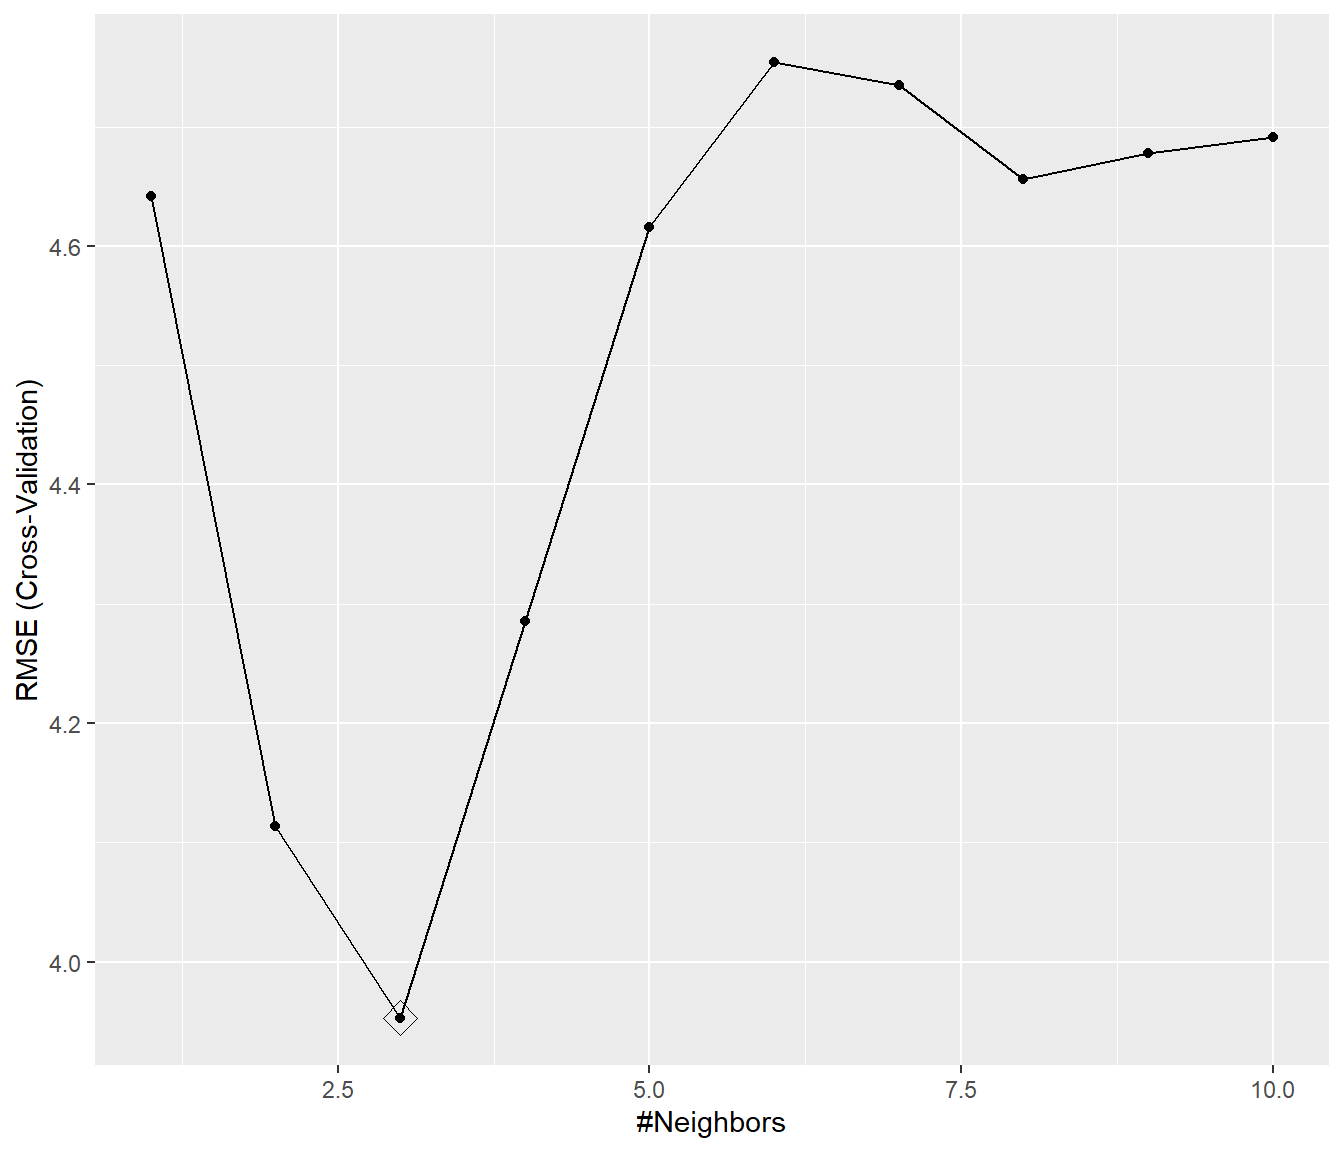
\includegraphics[width=0.8\linewidth]{01-introduccion_files/figure-latex/unnamed-chunk-24-2} \end{center}

\begin{Shaded}
\begin{Highlighting}[]
\NormalTok{knn}\OperatorTok{$}\NormalTok{bestTune}
\end{Highlighting}
\end{Shaded}

\begin{verbatim}
##   k
## 3 3
\end{verbatim}

\begin{Shaded}
\begin{Highlighting}[]
\NormalTok{knn}\OperatorTok{$}\NormalTok{finalModel}
\end{Highlighting}
\end{Shaded}

\begin{verbatim}
## 3-nearest neighbor regression model
\end{verbatim}

\begin{Shaded}
\begin{Highlighting}[]
\CommentTok{# Interpretación}
\KeywordTok{varImp}\NormalTok{(knn)}
\end{Highlighting}
\end{Shaded}

\begin{verbatim}
## loess r-squared variable importance
## 
##         Overall
## lstat    100.00
## rm        88.26
## indus     36.29
## ptratio   33.27
## tax       30.58
## crim      28.33
## nox       23.44
## black     21.29
## age       20.47
## rad       17.16
## zn        15.11
## dis       14.35
## chas       0.00
\end{verbatim}

\begin{Shaded}
\begin{Highlighting}[]
\CommentTok{# Evaluación}
\KeywordTok{postResample}\NormalTok{(}\KeywordTok{predict}\NormalTok{(knn, }\DataTypeTok{newdata =}\NormalTok{ test), test}\OperatorTok{$}\NormalTok{medv)}
\end{Highlighting}
\end{Shaded}

\begin{verbatim}
##     RMSE Rsquared      MAE 
## 4.960971 0.733945 2.724242
\end{verbatim}

Un comentario final:

\begin{quote}
``While I'm still supporting caret, the majority of my development
effort has gone into the tidyverse modeling packages (called
tidymodels)''.

--- Max Kuhn, autor del paquete \texttt{caret} (actualmente ingeniero de
software en RStudio).
\end{quote}

Kuhn, M. y Wickham, H. (2020). \emph{Tidymodels: a collection of
packages for modeling and machine learning using tidyverse principles}.
Version 0.1.1 (2020-07-14). \url{https://www.tidymodels.org}.

\chapter{Árboles de decisión}\label{trees}

Los \emph{árboles de decisión} son uno de los métodos más simples y
fáciles de interpretar para realizar predicciones en problemas de
clasificación y de regresión. Se desarrollan a partir de los años 70 del
siglo pasado como una alternativa versátil a los métodos clásicos de la
estadística, fuertemente basados en las hipótesis de linealidad y de
normalidad, y enseguida se convierten en una técnica básica del
aprendizaje automático. Aunque su calidad predictiva es mediocre
(especialmente en el caso de regresión), constituyen la base de otros
métodos altamente competitivos (bagging, bosques aleatorios, boosting)
en los que se combinan múltiples árboles para mejorar la predicción,
pagando el precio, eso sí, de hacer más difícil la interpretación del
modelo resultante.

La idea de este método consiste en la segmentación (partición) del
\emph{espacio predictor} (es decir, del conjunto de posibles valores de
las variables predictoras) en regiones tan simples que el proceso se
pueda representar mediante un árbol binario. Se parte de un nodo inicial
que representa a toda la muestra (se utiliza la muestra de
entrenamiento), del que salen dos ramas que dividen la muestra en dos
subconjuntos, cada uno representado por un nuevo nodo. Este proceso se
repite un número finito de veces hasta obtener las hojas del árbol, es
decir, los nodos terminales, que son los que se utilizan para realizar
la predicción. Una vez construido el árbol, la predicción se realizará
en cada nodo terminal utilizando, típicamente, la media en un problema
de regresión y la moda en un problema de clasificación.

\begin{center}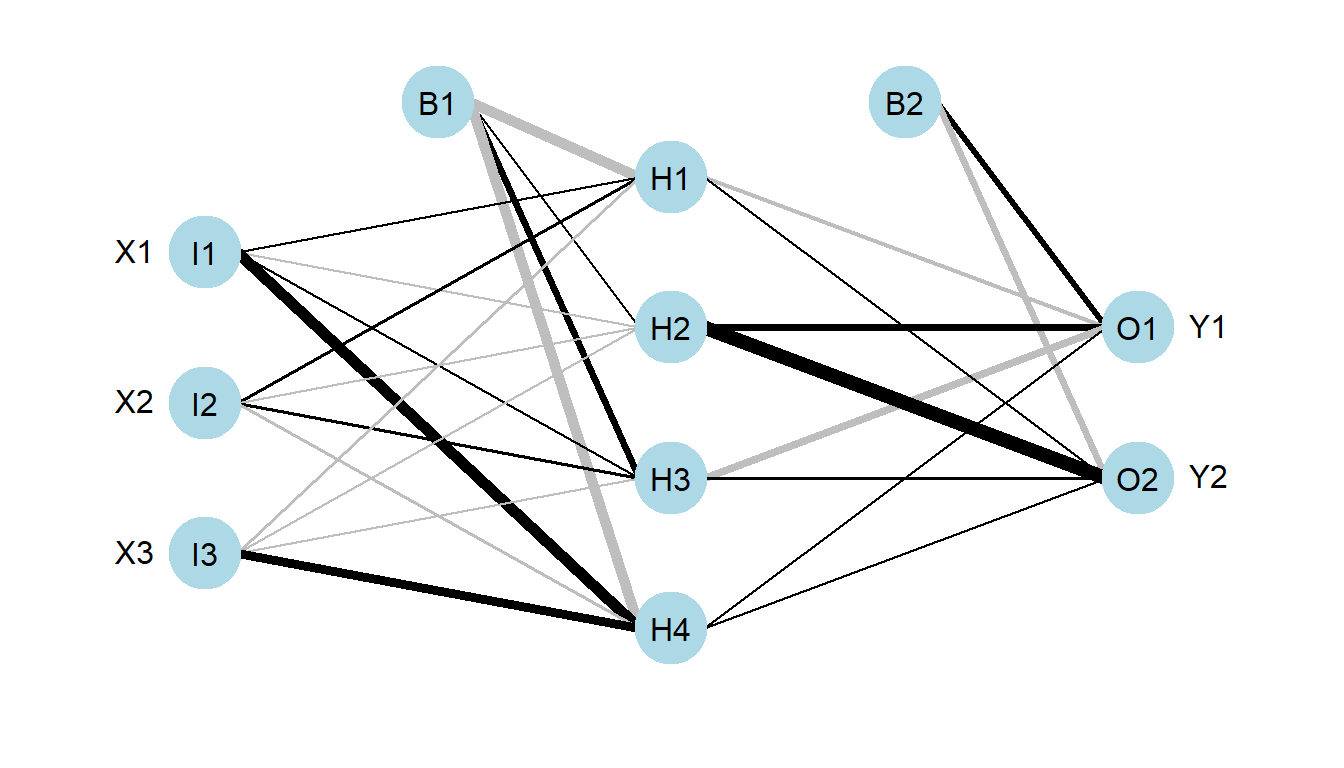
\includegraphics[width=0.8\linewidth]{02-arboles_files/figure-latex/unnamed-chunk-2-1} \end{center}

Al final de este proceso iterativo el espacio predictor se ha
particionado en regiones de forma rectangular en la que la predicción de
la respuesta es constante. Si la relación entre las variables
predictoras y la variable respuesta no se puede describir adecuadamente
mediante rectángulos, la calidad predictiva del árbol será limitada.
Como vemos, la simplicidad del modelo es su principal argumento, pero
también su talón de Aquiles.

\begin{center}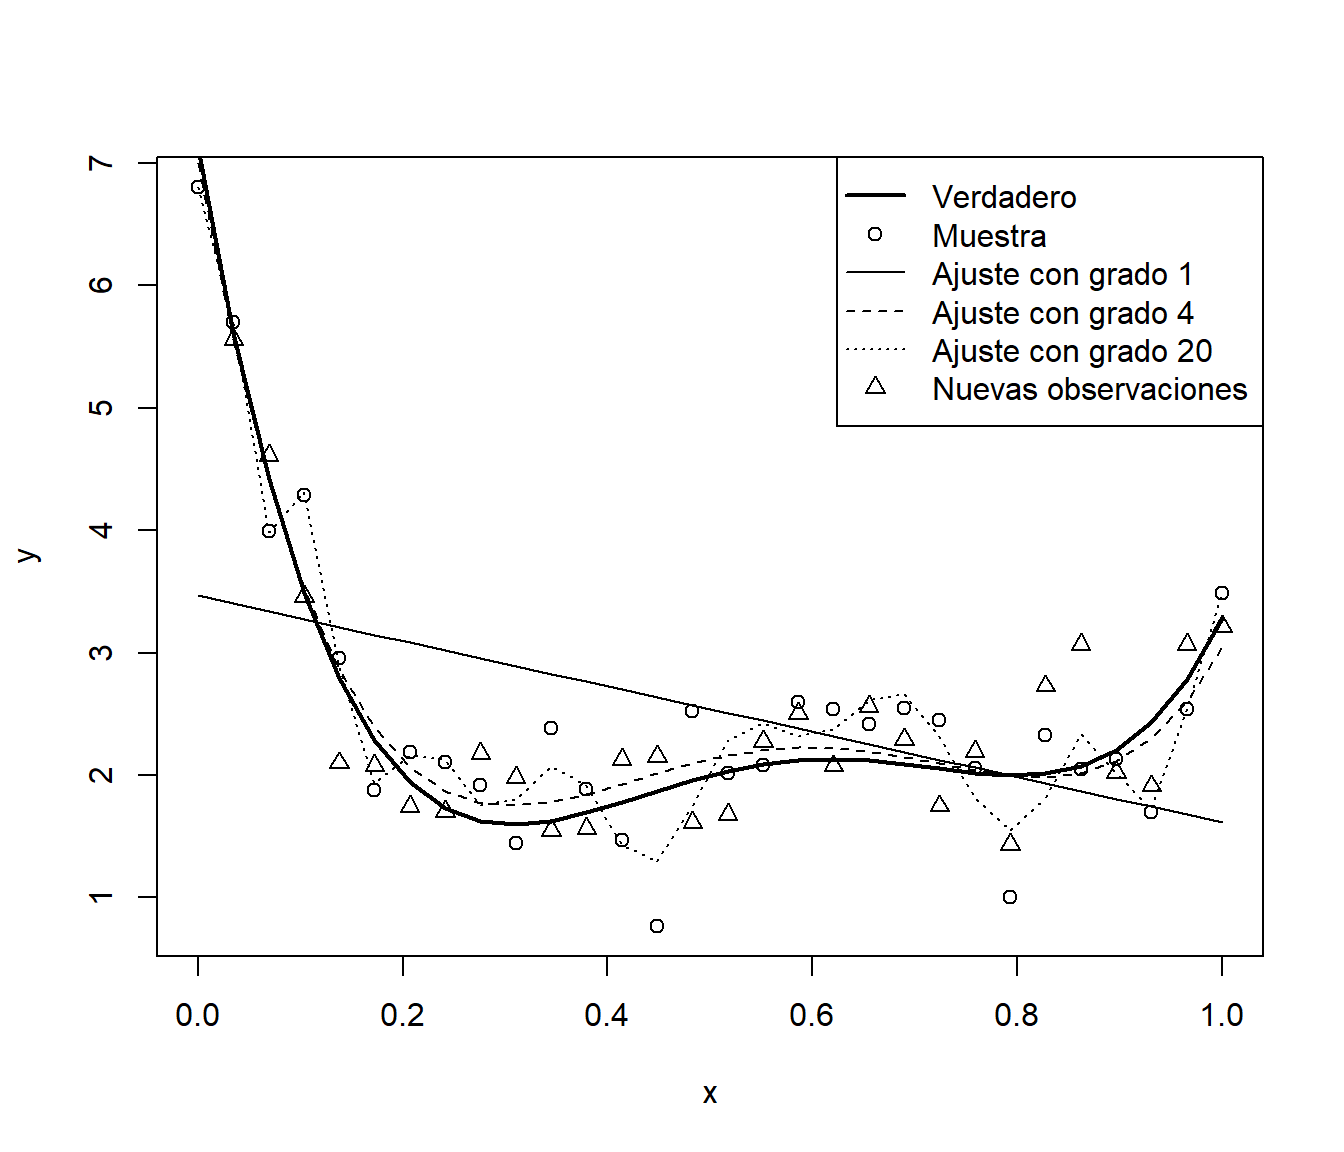
\includegraphics[width=0.8\linewidth]{02-arboles_files/figure-latex/unnamed-chunk-3-1} \end{center}

Como se ha dicho antes, cada nodo padre se divide, a través de dos
ramas, en dos nodos hijos. Esto se hace seleccionando una variable
predictora y dando respuesta a una pregunta dicotómica sobre ella. Por
ejemplo, ¿es el sueldo anual menor que 30000 euros?, o ¿es el género
igual a \emph{mujer}? Lo que se persigue con esta partición recursiva es
que los nodos terminales sean homogéneos respecto a la variable
respuesta \(Y\).

Por ejemplo, en un problema de clasificación, la homogeneidad de los
nodos terminales significaría que en cada uno de ellos sólo hay
elementos de una clase (categoría), y diríamos que los nodos son
\emph{puros}. En la práctica, esto siempre se puede conseguir
construyendo árboles suficientemente profundos, con muchas hojas. Pero
esta solución no es interesante, ya que va a dar lugar a un modelo
excesivamente complejo y por tanto sobreajustado y de difícil
interpretación. Será necesario encontrar un equilibrio entre la
complejidad del árbol y la pureza de los nodos terminales.

En resumen:

\begin{itemize}
\item
  Métodos simples y fácilmente interpretables.
\item
  Se representan mediante árboles binarios.
\item
  Técnica clásica de apendizaje automático (computación).
\item
  Válidos para regresión y para clasificación.
\item
  Válidos para predictores numéricos y categóricos.
\end{itemize}

La metodología CART (Classification and Regresion Trees, Breiman
\emph{et al.}, 1984) es la más popular para la construcción de árboles
de decisión y es la que se va a explicar con algo de detalle en las
siguientes secciones.

En primer lugar se tratarán los \emph{árboles de regresión} (árboles de
decisión en un problema de regresión, en el que la variable respuesta
\(Y\) es numérica) y después veremos los \emph{arboles de clasificación}
(respuesta categórica) que son los más utilizados en la práctica (los
primeros se suelen emplear únicamente como métodos descriptivos o como
base de métodos más complejos). Las variables predictoras
\(\mathbf{X}=(X_1, X_2, \ldots, X_p)\) pueden ser tanto numéricas como
categóricas. Además, con la metodología CART, las variables explicativas
podrían contener datos faltantes. Se pueden establecer ``particiones
sustitutas'' (\emph{surrogate splits}), de forma que cuando falta un
valor en una variable que determina una división, se usa una variable
alternativa que produce una partición similar.

\section{Árboles de regresión
CART}\label{uxe1rboles-de-regresiuxf3n-cart}

Como ya se comentó, la construcción del modelo se hace a partir de la
muestra de entrenamiento, y consiste en la partición del espacio
predictor en \(J\) regiones \(R_1, R_2, \ldots, R_J\), para cada una de
las cuales se va a calcular una constante: la media de la variable
respuesta \(Y\) para las observaciones de entranamiento que caen en la
región. Estas constantes son las que se van a utilizar para la
predicción de nuevas observaciones; para ello solo hay que comprobar
cuál es la región que le corresponde.

La cuestión clave es cómo se elige la partición del espacio predictor,
para lo que vamos a utilizar como criterio de error el RSS (suma de los
residuos al cuadrado). Como hemos dicho, vamos a modelizar la respuesta
en cada región como una constante, por tanto en la región \(R_j\) nos
interesa el \(min_{c_j} \sum_{i\in R_j} (y_i - c_j)^2\), que se alcanza
en la media de las respuestas \(y_i\) (de la muestra de entrenamiento)
en la región \(R_j\), a la que llamaremos \(\widehat y_{R_j}\). Por
tanto, se deben seleccionar las regiones \(R_1, R_2, \ldots, R_J\) que
minimicen

\[RSS = \sum_{j=1}^{J} \sum_{i\in R_j} (y_i - \widehat y_{R_j})^2\]
(Obsérvese el abuso de notación \(i\in R_j\), que significa las
observaciones \(i\in N\) que verifican \(x_i \in R_j\)).

Pero este problema es, en la práctica, intratable y vamos a tener que
simplificarlo. El método CART busca un compromiso entre rendimiento, por
una parte, y sencillez e interpretabilidad, por otra, y por ello en
lugar de hacer una búsqueda por todas las particiones posibles sigue un
proceso iterativo (recursivo) en el que va realizando cortes binarios.
En la primera iteración se trabaja con todos los datos:

\begin{itemize}
\item
  Una variable explicativa \(X_j\) y un punto de corte \(s\) definen dos
  hiperplanos \(R_1 = \{ X \mid X_j \le s \}\) y
  \(R_2 = \{ X \mid X_j > s \}\).
\item
  Se seleccionan los valores de \(j\) y \(s\) que minimizen
\end{itemize}

\[ \sum_{i\in R_1} (y_i - \widehat y_{R_1})^2 + \sum_{i\in R_2} (y_i - \widehat y_{R_2})^2\]

A diferencia del problema original, este se soluciona de forma muy
rápida. A continuación se repite el proceso en cada una de las dos
regiones \(R_1\) y \(R_2\), y así sucesivamente hasta alcanzar un
criterio de parada.

Fijémonos en que este método hace dos concesiones importantes: no solo
restringe la forma que pueden adoptar las particiones, sino que además
sigue un criterio de error \emph{greedy}: en cada iteración busca
minimizar el RSS de las dos regiones resultantes, sin preocuparse del
error que se va a cometer en iteraciones sucesivas. Y fijémonos también
en que este proceso se puede representar en forma de árbol binario (en
el sentido de que de cada nodo salen dos ramas, o ninguna cuando se
llega al final), de ahí la terminología de \emph{hacer crecer} el árbol.

¿Y cuándo paramos? Se puede parar cuando se alcance una profundidad
máxima, aunque lo más habitual es, para dividir un nodo (es decir, una
región), exigirle un número mínimo de observaciones.

\begin{itemize}
\item
  Si el árbol resultante es demasiado grande, va a ser un modelo
  demasiado complejo, por tanto va a ser difícil de interpretar y, sobre
  todo, va a provocar un sobreajuste de los datos. Cuando se evalúe el
  rendimiento utilizando la muestra de validación, los resultados van a
  ser malos. Dicho de otra manera, tendremos un modelo con poco sesgo
  pero con mucha varianza y en consecuencia inestable (pequeños cambios
  en los datos darán lugar a modelos muy distintos). Más adelante
  veremos que esto justifica la utilización del \emph{bagging} como
  técnica para reducir la varianza.
\item
  Si el árbol es demasiado pequeño, va a tener menos varianza (menos
  inestable) a costa de más sesgo. Más adelante veremos que esto
  justifica la utilización del \emph{boosting}. Los árboles pequeños son
  más fáciles de interpretar ya que permiten identificar las variables
  explicativas que más influyen en la predicción.
\end{itemize}

Sin entrar por ahora en métodos combinados (métodos \emph{ensemble},
tipo \emph{bagging} o \emph{boosting}), vamos a explicar cómo encontrar
un equilibrio entre sesgo y varianza. Lo que se hace es construir un
árbol grande para a continuación empezar a \emph{podarlo}. Podar un
árbol significa colapsar cualquier cantidad de sus nodos internos (no
terminales), dando lugar a otro árbol más pequeño al que llamaremos
\emph{subárbol} del árbol original. Sabemos que el árbol completo es el
que va a tener menor error si utilizamos la muestra de entrenamiento,
pero lo que realmente nos interesa es encontrar el subárbol con un menor
error al utilizar la muestra de validación. Lamentablemente, no es una
buena estrategia el evaluar todos los subárboles: simplemente, hay
demasiados. Lo que se hace es, mediante un hiperparámetro (\emph{tuning
parameter} o parámetro de ajuste) controlar el tamaño del árbol, es
decir, la complejidad del modelo, seleccionando el subárbol
\emph{optimo} (para los datos de los que disponemos, claro). Veamos la
idea.

Dado un subárbol \(T\) con \(R_1, R_2, \ldots, R_t\) nodos terminales,
consideramos como medida del error el RSS más una penalización que
depende de un hiperparámetro no negativo \(\alpha \ge 0\)

\begin{equation} 
RSS_{\alpha} = \sum_{j=1}^t \sum_{i\in R_j} (y_i - \widehat y_{R_j})^2 + \alpha t
\label{eq:rss-alpha}
\end{equation}

Para cada valor del parámetro \(\alpha\) existe un único subárbol
\emph{más pequeño} que minimiza este error (obsérvese que aunque hay un
continuo de valores distinos de \(\alpha\), sólo hay una cantidad finita
de subárboles). Evidentemente, cuando \(\alpha = 0\), ese subárbol será
el árbol completo, algo que no nos interesa. Pero a medida que se
incrementa \(\alpha\) se penalizan los subárboles con muchos nodos
terminales, dando lugar a una solución más pequeña. Encontrarla puede
parecer muy costoso computacionalmente, pero lo cierto es que no lo es.
El algoritmo consistente en ir colapsando nodos de forma sucesiva, de
cada vez el nodo que produzca el menor incremento en el RSS (corregido
por un factor que depende del tamaño), da lugar a una sucesión finita de
subárboles que contiene, para todo \(\alpha\), la solución.

Para finalizar, sólo resta seleccionar un valor de \(\alpha\). Para
ello, como se comentó en la Sección \ref{entrenamiento-test}, se podría
dividir la muestra en tres subconjuntos: datos de entrenamiento, de
validación y de test. Para cada valor del parámetro de complejidad
\(\alpha\) hemos utilizado la muestra de entrenamiento para obtener un
árbol (en la jerga, para cada valor del hiperparámetro \(\alpha\) se
entrena un modelo). Se emplea la muestra independiente de validación
para seleccionar el valor de \(\alpha\) (y por tanto el árbol) con el
que nos quedamos. Y por último emplearemos la muestra de test
(independiente de las otras dos) para evaluar el rendimiento del árbol
seleccionado. No obstante, lo más habitual para seleccionar el valor del
hiperparámetro \(\alpha\) es emplear validación cruzada (o otro tipo de
remuestreo) en la muestra de entrenamiento en lugar de considerar una
muestra adicional de validación.

Hay dos opciones muy utilizadas en la práctica para seleccionar el valor
de \(\alpha\): se puede utilizar directamente el valor que minimice el
error; o se puede forzar que el modelo sea un poco más sencillo con la
regla \emph{one-standard-error}, que selecciona el árbol más pequeño que
esté a una distancia de un error estándar del árbol obtenido mediante la
opción anterior.

También es habitual escribir la Ecuación \eqref{eq:rss-alpha} reescalando
el parámetro de complejidad como \(\tilde \alpha = \alpha / RSS_0\),
siendo \(RSS_0 = \sum_{i=1}^{n} (y_i - \bar y)^2\) la variabilidad total
(la suma de cuadrados residual del árbol sin divisiones):
\[RSS_{\tilde \alpha}=RSS + \tilde \alpha RSS_0 t\]

De esta forma se podría interpretar el hiperparámetro \(\tilde \alpha\)
como una penalización en la proporción de variabilidad explicada, ya que
dividiendo la expresión anterior por \(RSS_0\) obtendríamos:
\[R^2_{\tilde \alpha}=R^2+ \tilde \alpha  t\]

\section{Árboles de clasificación
CART}\label{uxe1rboles-de-clasificaciuxf3n-cart}

En un problema de clasificación la variable respuesta puede tomar los
valores \(1, 2, \ldots, K\), etiquetas que identifican las \(K\)
categorías del problema. Una vez construido el árbol, se comprueba cuál
es la categoría modal de cada región: considerando la muestra de
entrenamiento, la categoría más frecuente. Dada una observación, se
predice que pertenece a la categoría modal de la región a la que
pertenece.

El resto del proceso es idéntico al de los árboles de regresión ya
explicado, con una única salvedad: no podemos utilizar RSS como medida
del error. Es necesario buscar una medida del error adaptada a este
contexto. Fijada una región, vamos a denotar por \(\widehat p_{k}\), con
\(k = 1, 2, \ldots, K\), a la proporción de observaciones (de la muestra
de entrenamiento) en la región que pertenecen a la categoría \(k\). Se
utilizan tres medidas distintas del error en la región:

\begin{itemize}
\item
  Proporción de errores de clasificación:
  \[1 - max_{k} (\widehat p_{k})\]
\item
  Índice de Gini: \[\sum_{k=1}^K \widehat p_{k} (1 - \widehat p_{k})\]
\item
  Entropía\footnote{La entropía es un concepto básico de la teoría de la
    información (Shannon, 1948) y se mide en \emph{bits} (cuando en la
    definición se utilizan \(log_2\)).} (\emph{cross-entropy}):
  \[- \sum_{k=1}^K \widehat p_{k} \text{log}(\widehat p_{k})\]
\end{itemize}

Aunque la proporción de errores de clasificación es la medida del error
más intuitiva, en la práctica sólo se utiliza para la fase de poda.
Fijémonos que en el cálculo de esta medida sólo interviene
\(max_{k} (\widehat p_{k})\), mientras que en las medidas alternativas
intervienen las proporciones \(\widehat p_{k}\) de todas las categorías.
Para la fase de crecimiento se utilizan indistintamente el índice de
Gini o la entropía. Cuando nos interesa el error no en una única región
sino en varias (al romper un nodo en dos, o al considerar todos los
nodos terminales), se suman los errores de cada región previa
ponderación por el número de observaciones que hay en cada una de ellas.

En la introducción de este tema se comentó que los árboles de decisión
admiten tanto variables predictoras numéricas como categóricas, y esto
es cierto tanto para árboles de regresión como para árboles de
clasificación. Veamos brevemente como se tratarían los predictores
categóricos a la hora de incorporarlos al árbol. El problema radica en
qué se entiende por hacer un corte si las categorías del predictor no
están ordenadas. Hay dos soluciones básicas:

\begin{itemize}
\item
  Definir variables predictoras \emph{dummy}. Se trata de variables
  indicadoras, una por cada una de las categorías que tiene el
  predictor. Este criterio de \emph{uno contra todos} tiene la ventaja
  de que estas variables son fácilmente interpretables, pero tiene el
  inconveniente de que puede aumentar mucho el número de variables
  predictoras.
\item
  Ordenar las categorías de la variable predictora. Lo ideal sería
  considerar todas las ordenaciones posibles, pero eso es desde luego
  poco práctico: el incremento es factorial. El truco consiste en
  utilizar un único órden basado en algún criterio \emph{greedy}. Por
  ejemplo, si la variable respuesta \(Y\) también es categórica, se
  puede seleccionar una de sus categorías que resulte especialmente
  interesante y ordenar las categorías del predictor según su proporción
  en la categoría de \(Y\). Este enfoque no añade complejidad al modelo,
  pero puede dar lugar a resultados de difícil interpretación.
\end{itemize}

\section{\texorpdfstring{CART con el paquete
\texttt{rpart}}{CART con el paquete rpart}}\label{cart-con-el-paquete-rpart}

La metodología CART está implementada en el paquete
\href{https://CRAN.R-project.org/package=rpart}{\texttt{rpart}}
(Recursive PARTitioning)\footnote{El paquete
  \href{https://CRAN.R-project.org/package=tree}{\texttt{tree}} es una
  traducción del original en S.}. La función principal es
\texttt{rpart()} y habitualmente se emplea de la forma:

\texttt{rpart(formula,\ data,\ method,\ parms,\ control,\ ...)}

\begin{itemize}
\item
  \texttt{formula}: permite especificar la respuesta y las variables
  predictoras de la forma habitual, se suele establecer de la forma
  \texttt{respuesta\ \textasciitilde{}\ .} para incluir todas las
  posibles variables explicativas.
\item
  \texttt{data}: \texttt{data.frame} (opcional; donde se evaluará la
  fórmula) con la muestra de entrenamiento.
\item
  \texttt{method}: método empleado para realizar las particiones, puede
  ser \texttt{"anova"} (regresión), \texttt{"class"} (clasificación),
  \texttt{"poisson"} (regresión de Poisson) o \texttt{"exp"}
  (supervivencia), o alternativamente una lista de funciones (con
  componentes \texttt{init}, \texttt{split}, \texttt{eval}; ver la
  vignette
  \href{https://cran.r-project.org/web/packages/rpart/vignettes/usercode.pdf}{\emph{User
  Written Split Functions}}). Por defecto se selecciona a partir de la
  variable respuesta en \texttt{formula}, por ejemplo si es un factor
  (lo recomendado en clasificación) emplea \texttt{method\ =\ "class"}.
\item
  \texttt{parms}: lista de parámetros opcionales para la partición en el
  caso de clasificación (o regresión de Poisson). Puede contener los
  componentes \texttt{prior} (vector de probabilidades previas; por
  defecto las frecuencias observadas), \texttt{loss} (matriz de
  pérdidas; con ceros en la diagonal y por defecto 1 en el resto) y
  \texttt{split} (criterio de error; por defecto \texttt{"gini"} o
  alternativamente \texttt{"information"}).
\item
  \texttt{control}: lista de opciones que controlan el algoritmo de
  partición, por defecto se seleccionan mediante la función
  \texttt{rpart.control}, aunque también se pueden establecer en la
  llamada a la función principal, y los principales parámetros son:

  \texttt{rpart.control(minsplit\ =\ 20,\ minbucket\ =\ round(minsplit/3),\ cp\ =\ 0.01,\ xval\ =\ 10,\ maxdepth\ =\ 30,\ ...)}

  \begin{itemize}
  \item
    \texttt{cp} es el parámetro de complejidad \(\tilde \alpha\) para la
    poda del árbol, de forma que un valor de 1 se corresponde con un
    árbol sin divisiones y un valor de 0 con un árbol de profundidad
    máxima. Adicionalmente, para reducir el tiempo de computación, el
    algoritmo empleado no realiza una partición si la proporción de
    reducción del error es inferior a este valor (valores más grandes
    simplifican el modelo y reducen el tiempo de computación).
  \item
    \texttt{maxdepth} es la profundidad máxima del árbol (la profundidad
    de la raíz sería 0).
  \item
    \texttt{minsplit} y \texttt{minbucket} son, respectivamente, los
    números mínimos de observaciones en un nodo intermedio para
    particionarlo y en un nodo terminal.
  \item
    \texttt{xval} es el número de grupos (folds) para validación
    cruzada.
  \end{itemize}
\end{itemize}

Para más detalles consultar la documentación de esta función o la
vignette
\href{https://cran.r-project.org/web/packages/rpart/vignettes/longintro.pdf}{\emph{Introduction
to Rpart}}.

\subsection{Ejemplo: regresión}\label{ejemplo-regresiuxf3n}

Emplearemos el conjunto de datos \emph{winequality.RData} (ver Cortez et
al., 2009), que contiene información fisico-química
(\texttt{fixed.acidity}, \texttt{volatile.acidity},
\texttt{citric.acid}, \texttt{residual.sugar}, \texttt{chlorides},
\texttt{free.sulfur.dioxide}, \texttt{total.sulfur.dioxide},
\texttt{density}, \texttt{pH}, \texttt{sulphates} y \texttt{alcohol}) y
sensorial (\texttt{quality}) de una muestra de 1250 vinos portugueses de
la variedad \emph{Vinho Verde}. Como respuesta consideraremos la
variable \texttt{quality}, mediana de al menos 3 evaluaciones de la
calidad del vino realizadas por expertos, que los evaluaron entre 0 (muy
malo) y 10 (muy excelente).

\begin{Shaded}
\begin{Highlighting}[]
\KeywordTok{load}\NormalTok{(}\StringTok{"data/winequality.RData"}\NormalTok{)}
\KeywordTok{str}\NormalTok{(winequality)}
\end{Highlighting}
\end{Shaded}

\begin{verbatim}
## 'data.frame':    1250 obs. of  12 variables:
##  $ fixed.acidity       : num  6.8 7.1 6.9 7.5 8.6 7.7 5.4 6.8 6.1 5.5 ...
##  $ volatile.acidity    : num  0.37 0.24 0.32 0.23 0.36 0.28 0.59 0.16 0.28 0.28 ...
##  $ citric.acid         : num  0.47 0.34 0.13 0.49 0.26 0.63 0.07 0.36 0.27 0.21 ...
##  $ residual.sugar      : num  11.2 1.2 7.8 7.7 11.1 11.1 7 1.3 4.7 1.6 ...
##  $ chlorides           : num  0.071 0.045 0.042 0.049 0.03 0.039 0.045 0.034 0.03 0.032 ...
##  $ free.sulfur.dioxide : num  44 6 11 61 43.5 58 36 32 56 23 ...
##  $ total.sulfur.dioxide: num  136 132 117 209 171 179 147 98 140 85 ...
##  $ density             : num  0.997 0.991 0.996 0.994 0.995 ...
##  $ pH                  : num  2.98 3.16 3.23 3.14 3.03 3.08 3.34 3.02 3.16 3.42 ...
##  $ sulphates           : num  0.88 0.46 0.37 0.3 0.49 0.44 0.57 0.58 0.42 0.42 ...
##  $ alcohol             : num  9.2 11.2 9.2 11.1 12 8.8 9.7 11.3 12.5 12.5 ...
##  $ quality             : int  5 4 5 7 5 4 6 6 8 5 ...
\end{verbatim}

\begin{Shaded}
\begin{Highlighting}[]
\KeywordTok{barplot}\NormalTok{(}\KeywordTok{table}\NormalTok{(winequality}\OperatorTok{$}\NormalTok{quality))}
\end{Highlighting}
\end{Shaded}

\begin{center}\includegraphics[width=0.8\linewidth]{02-arboles_files/figure-latex/unnamed-chunk-4-1} \end{center}

En primer lugar se selecciona el 80\% de los datos como muestra de
entrenamiento y el 20\% restante como muestra de test:

\begin{Shaded}
\begin{Highlighting}[]
\KeywordTok{set.seed}\NormalTok{(}\DecValTok{1}\NormalTok{)}
\NormalTok{nobs <-}\StringTok{ }\KeywordTok{nrow}\NormalTok{(winequality)}
\NormalTok{itrain <-}\StringTok{ }\KeywordTok{sample}\NormalTok{(nobs, }\FloatTok{0.8} \OperatorTok{*}\StringTok{ }\NormalTok{nobs)}
\NormalTok{train <-}\StringTok{ }\NormalTok{winequality[itrain, ]}
\NormalTok{test <-}\StringTok{ }\NormalTok{winequality[}\OperatorTok{-}\NormalTok{itrain, ]}
\end{Highlighting}
\end{Shaded}

Podemos obtener el arbol con las opciones por defecto con el comando:

\begin{Shaded}
\begin{Highlighting}[]
\NormalTok{tree <-}\StringTok{ }\KeywordTok{rpart}\NormalTok{(quality }\OperatorTok{~}\StringTok{ }\NormalTok{., }\DataTypeTok{data =}\NormalTok{ train)}
\end{Highlighting}
\end{Shaded}

Al imprimirlo se muestra el número de observaciones e información sobre
los distintos nodos (número de nodo, condición que define la partición,
número de observaciones en el nodo, función de pérdida y predicción),
marcando con un \texttt{*} los nodos terminales.

\begin{Shaded}
\begin{Highlighting}[]
\NormalTok{tree}
\end{Highlighting}
\end{Shaded}

\begin{verbatim}
## n= 1000 
## 
## node), split, n, deviance, yval
##       * denotes terminal node
## 
##  1) root 1000 768.95600 5.862000  
##    2) alcohol< 10.75 622 340.81190 5.586817  
##      4) volatile.acidity>=0.2575 329 154.75990 5.370821  
##        8) total.sulfur.dioxide< 98.5 24  12.50000 4.750000 *
##        9) total.sulfur.dioxide>=98.5 305 132.28200 5.419672  
##         18) pH< 3.315 269 101.44980 5.353160 *
##         19) pH>=3.315 36  20.75000 5.916667 *
##      5) volatile.acidity< 0.2575 293 153.46760 5.829352  
##       10) sulphates< 0.475 144  80.32639 5.659722 *
##       11) sulphates>=0.475 149  64.99329 5.993289 *
##    3) alcohol>=10.75 378 303.53700 6.314815  
##      6) alcohol< 11.775 200 173.87500 6.075000  
##       12) free.sulfur.dioxide< 11.5 15  10.93333 4.933333 *
##       13) free.sulfur.dioxide>=11.5 185 141.80540 6.167568  
##         26) volatile.acidity>=0.395 7  12.85714 5.142857 *
##         27) volatile.acidity< 0.395 178 121.30900 6.207865  
##           54) citric.acid>=0.385 31  21.93548 5.741935 *
##           55) citric.acid< 0.385 147  91.22449 6.306122 *
##      7) alcohol>=11.775 178 105.23600 6.584270 *
\end{verbatim}

Para representarlo se puede emplear las herramientas del paquete
\href{https://CRAN.R-project.org/package=rpart}{\texttt{rpart}}:

\begin{Shaded}
\begin{Highlighting}[]
\KeywordTok{plot}\NormalTok{(tree)}
\KeywordTok{text}\NormalTok{(tree)}
\end{Highlighting}
\end{Shaded}

\begin{center}\includegraphics[width=0.8\linewidth]{02-arboles_files/figure-latex/unnamed-chunk-8-1} \end{center}

Pero puede ser preferible emplear el paquete
\href{https://CRAN.R-project.org/package=rpart.plot}{\texttt{rpart.plot}}

\begin{Shaded}
\begin{Highlighting}[]
\KeywordTok{library}\NormalTok{(rpart.plot)}
\KeywordTok{rpart.plot}\NormalTok{(tree, }\DataTypeTok{main=}\StringTok{"Regresion tree winequality"}\NormalTok{)  }
\end{Highlighting}
\end{Shaded}

\begin{center}\includegraphics[width=0.8\linewidth]{02-arboles_files/figure-latex/unnamed-chunk-9-1} \end{center}

Nos interesa como se clasificaría a una nueva observación en los nodos
terminales (en los nodos intermedios solo nos interesarían las
condiciones, y el orden de las variables consideradas, hasta llegar a
las hojas) y las correspondientes predicciones (la media de la respuesta
en el correspondiente nodo terminal). Para ello, puede ser de utilidad
imprimir las reglas:

\begin{Shaded}
\begin{Highlighting}[]
\KeywordTok{rpart.rules}\NormalTok{(tree, }\DataTypeTok{style =} \StringTok{"tall"}\NormalTok{)}
\end{Highlighting}
\end{Shaded}

\begin{verbatim}
## quality is 4.8 when
##     alcohol < 11
##     volatile.acidity >= 0.26
##     total.sulfur.dioxide < 99
## 
## quality is 4.9 when
##     alcohol is 11 to 12
##     free.sulfur.dioxide < 12
## 
## quality is 5.1 when
##     alcohol is 11 to 12
##     volatile.acidity >= 0.40
##     free.sulfur.dioxide >= 12
## 
## quality is 5.4 when
##     alcohol < 11
##     volatile.acidity >= 0.26
##     total.sulfur.dioxide >= 99
##     pH < 3.3
## 
## quality is 5.7 when
##     alcohol < 11
##     volatile.acidity < 0.26
##     sulphates < 0.48
## 
## quality is 5.7 when
##     alcohol is 11 to 12
##     volatile.acidity < 0.40
##     free.sulfur.dioxide >= 12
##     citric.acid >= 0.39
## 
## quality is 5.9 when
##     alcohol < 11
##     volatile.acidity >= 0.26
##     total.sulfur.dioxide >= 99
##     pH >= 3.3
## 
## quality is 6.0 when
##     alcohol < 11
##     volatile.acidity < 0.26
##     sulphates >= 0.48
## 
## quality is 6.3 when
##     alcohol is 11 to 12
##     volatile.acidity < 0.40
##     free.sulfur.dioxide >= 12
##     citric.acid < 0.39
## 
## quality is 6.6 when
##     alcohol >= 12
\end{verbatim}

Por defecto se poda el arbol considerando \texttt{cp\ =\ 0.01}, que
puede ser adecuado en muchos casos. Sin embargo, para seleccionar el
valor óptimo de este (hiper)parámetro se puede emplear validación
cruzada. En primer lugar habría que establecer \texttt{cp\ =\ 0} para
construir el árbol completo, a la profundidad máxima (determinada por
los valores de \texttt{minsplit} y \texttt{minbucket}, que se podrían
seleccionar ``a mano'' dependiendo del número de observaciones o también
considerándolos como hiperparámetos; esto último no está implementado en
\texttt{rpart}, ni en principio en \texttt{caret})\footnote{Los
  parámetros \texttt{maxsurrogate}, \texttt{usesurrogate} y
  \texttt{surrogatestyle} serían de utilidad si hay datos faltantes.}.

\begin{Shaded}
\begin{Highlighting}[]
\NormalTok{tree <-}\StringTok{ }\KeywordTok{rpart}\NormalTok{(quality }\OperatorTok{~}\StringTok{ }\NormalTok{., }\DataTypeTok{data =}\NormalTok{ train, }\DataTypeTok{cp =} \DecValTok{0}\NormalTok{)}
\end{Highlighting}
\end{Shaded}

Posteriormente podemos emplear las funciones \texttt{printcp()} (o
\texttt{plotcp()}) para obtener (representar) los valores de CP para los
árboles (óptimos) de menor tamaño junto con su error de validación
cruzada \texttt{xerror} (reescalado de forma que el máximo de
\texttt{rel\ error} es 1):

\begin{Shaded}
\begin{Highlighting}[]
\KeywordTok{printcp}\NormalTok{(tree)}
\end{Highlighting}
\end{Shaded}

\begin{verbatim}
## 
## Regression tree:
## rpart(formula = quality ~ ., data = train, cp = 0)
## 
## Variables actually used in tree construction:
##  [1] alcohol              chlorides            citric.acid         
##  [4] density              fixed.acidity        free.sulfur.dioxide 
##  [7] pH                   residual.sugar       sulphates           
## [10] total.sulfur.dioxide volatile.acidity    
## 
## Root node error: 768.96/1000 = 0.76896
## 
## n= 1000 
## 
##            CP nsplit rel error  xerror     xstd
## 1  0.16204707      0   1.00000 1.00203 0.048591
## 2  0.04237491      1   0.83795 0.85779 0.043646
## 3  0.03176525      2   0.79558 0.82810 0.043486
## 4  0.02748696      3   0.76381 0.81350 0.042814
## 5  0.01304370      4   0.73633 0.77038 0.039654
## 6  0.01059605      6   0.71024 0.78168 0.039353
## 7  0.01026605      7   0.69964 0.78177 0.039141
## 8  0.00840800      9   0.67911 0.78172 0.039123
## 9  0.00813924     10   0.67070 0.80117 0.039915
## 10 0.00780567     11   0.66256 0.80020 0.040481
## 11 0.00684175     13   0.64695 0.79767 0.040219
## 12 0.00673843     15   0.63327 0.81381 0.040851
## 13 0.00643577     18   0.61305 0.82059 0.041240
## 14 0.00641137     19   0.60662 0.82323 0.041271
## 15 0.00549694     21   0.59379 0.84187 0.042714
## 16 0.00489406     23   0.58280 0.84748 0.042744
## 17 0.00483045     24   0.57791 0.85910 0.043897
## 18 0.00473741     25   0.57308 0.86553 0.045463
## 19 0.00468372     26   0.56834 0.86455 0.045413
## 20 0.00450496     28   0.55897 0.87049 0.045777
## 21 0.00448365     32   0.54095 0.87263 0.045824
## 22 0.00437484     33   0.53647 0.87260 0.045846
## 23 0.00435280     35   0.52772 0.87772 0.046022
## 24 0.00428623     36   0.52337 0.87999 0.046124
## 25 0.00412515     37   0.51908 0.88151 0.046505
## 26 0.00390866     39   0.51083 0.89242 0.047068
## 27 0.00375301     42   0.49910 0.90128 0.047319
## 28 0.00370055     43   0.49535 0.90965 0.047991
## 29 0.00351987     45   0.48795 0.91404 0.048079
## 30 0.00308860     47   0.48091 0.92132 0.048336
## 31 0.00305781     49   0.47473 0.93168 0.049699
## 32 0.00299018     51   0.46862 0.93258 0.049701
## 33 0.00295148     52   0.46563 0.93062 0.049644
## 34 0.00286138     54   0.45972 0.93786 0.050366
## 35 0.00283972     55   0.45686 0.93474 0.050404
## 36 0.00274809     56   0.45402 0.93307 0.050390
## 37 0.00273457     58   0.44853 0.93642 0.050406
## 38 0.00260607     59   0.44579 0.93726 0.050543
## 39 0.00252978     60   0.44318 0.93692 0.050323
## 40 0.00252428     62   0.43813 0.93778 0.050381
## 41 0.00250804     64   0.43308 0.93778 0.050381
## 42 0.00232226     65   0.43057 0.93642 0.050081
## 43 0.00227625     66   0.42825 0.93915 0.050166
## 44 0.00225146     67   0.42597 0.94101 0.050195
## 45 0.00224774     68   0.42372 0.94101 0.050195
## 46 0.00216406     69   0.42147 0.94067 0.050124
## 47 0.00204851     70   0.41931 0.94263 0.050366
## 48 0.00194517     72   0.41521 0.94203 0.050360
## 49 0.00188139     73   0.41326 0.93521 0.050349
## 50 0.00154129     75   0.40950 0.93500 0.050277
## 51 0.00143642     76   0.40796 0.93396 0.050329
## 52 0.00118294     77   0.40652 0.93289 0.050325
## 53 0.00117607     78   0.40534 0.93738 0.050406
## 54 0.00108561     79   0.40417 0.93738 0.050406
## 55 0.00097821     80   0.40308 0.93670 0.050406
## 56 0.00093107     81   0.40210 0.93752 0.050589
## 57 0.00090075     82   0.40117 0.93752 0.050589
## 58 0.00082968     83   0.40027 0.93634 0.050561
## 59 0.00048303     85   0.39861 0.93670 0.050557
## 60 0.00000000     86   0.39813 0.93745 0.050558
\end{verbatim}

\begin{Shaded}
\begin{Highlighting}[]
\KeywordTok{plotcp}\NormalTok{(tree)}
\end{Highlighting}
\end{Shaded}

\begin{center}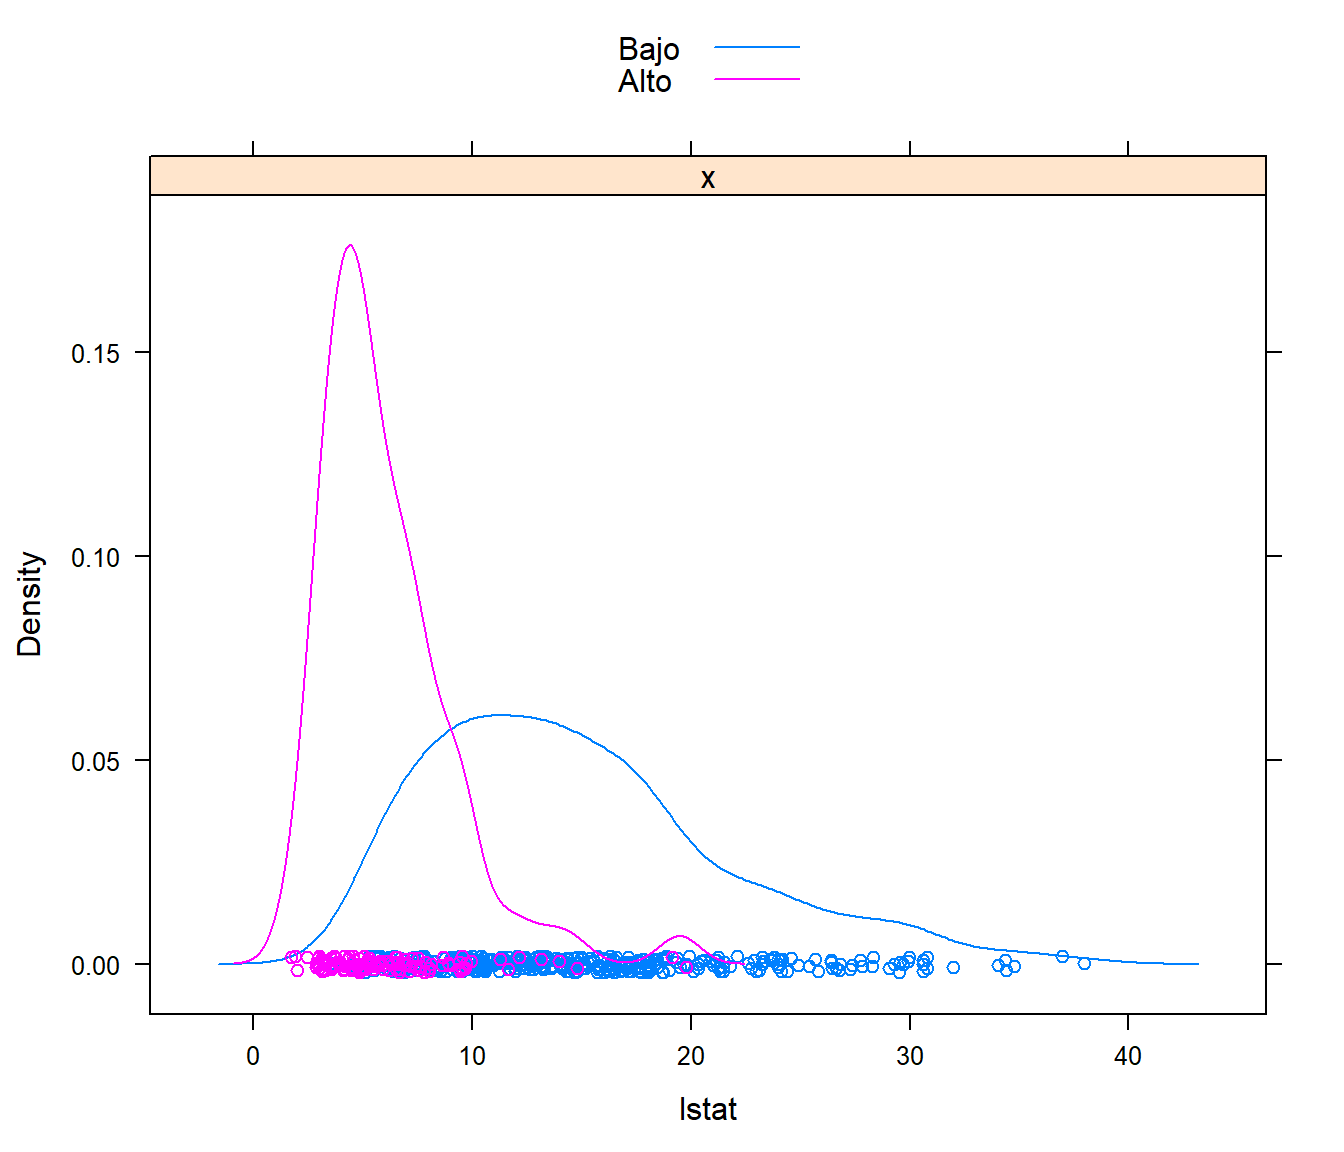
\includegraphics[width=0.8\linewidth]{02-arboles_files/figure-latex/unnamed-chunk-12-1} \end{center}

La tabla con los valores de las podas (óptimas, dependiendo del
parámetro de complejidad) está almacenada en la componente
\texttt{\$cptable}:

\begin{Shaded}
\begin{Highlighting}[]
\KeywordTok{head}\NormalTok{(tree}\OperatorTok{$}\NormalTok{cptable, }\DecValTok{10}\NormalTok{)}
\end{Highlighting}
\end{Shaded}

\begin{verbatim}
##             CP nsplit rel error    xerror       xstd
## 1  0.162047069      0 1.0000000 1.0020304 0.04859127
## 2  0.042374911      1 0.8379529 0.8577876 0.04364585
## 3  0.031765253      2 0.7955780 0.8281010 0.04348571
## 4  0.027486958      3 0.7638128 0.8134957 0.04281430
## 5  0.013043701      4 0.7363258 0.7703804 0.03965433
## 6  0.010596054      6 0.7102384 0.7816774 0.03935308
## 7  0.010266055      7 0.6996424 0.7817716 0.03914071
## 8  0.008408003      9 0.6791102 0.7817177 0.03912344
## 9  0.008139238     10 0.6707022 0.8011719 0.03991498
## 10 0.007805674     11 0.6625630 0.8001996 0.04048088
\end{verbatim}

A partir de la que podríamos seleccionar el valor óptimo de forma
automática, siguiendo el criterio de un error estándar de Breiman et al.
(1984):

\begin{Shaded}
\begin{Highlighting}[]
\NormalTok{xerror <-}\StringTok{ }\NormalTok{tree}\OperatorTok{$}\NormalTok{cptable[,}\StringTok{"xerror"}\NormalTok{]}
\NormalTok{imin.xerror <-}\StringTok{ }\KeywordTok{which.min}\NormalTok{(xerror)}
\CommentTok{# Valor óptimo}
\NormalTok{tree}\OperatorTok{$}\NormalTok{cptable[imin.xerror, ]}
\end{Highlighting}
\end{Shaded}

\begin{verbatim}
##         CP     nsplit  rel error     xerror       xstd 
## 0.01304370 4.00000000 0.73632581 0.77038039 0.03965433
\end{verbatim}

\begin{Shaded}
\begin{Highlighting}[]
\CommentTok{# Límite superior "oneSE rule" y complejidad mínima por debajo de ese valor}
\NormalTok{upper.xerror <-}\StringTok{ }\NormalTok{xerror[imin.xerror] }\OperatorTok{+}\StringTok{ }\NormalTok{tree}\OperatorTok{$}\NormalTok{cptable[imin.xerror, }\StringTok{"xstd"}\NormalTok{]}
\NormalTok{icp <-}\StringTok{ }\KeywordTok{min}\NormalTok{(}\KeywordTok{which}\NormalTok{(xerror }\OperatorTok{<=}\StringTok{ }\NormalTok{upper.xerror))}
\NormalTok{cp <-}\StringTok{ }\NormalTok{tree}\OperatorTok{$}\NormalTok{cptable[icp, }\StringTok{"CP"}\NormalTok{]}
\end{Highlighting}
\end{Shaded}

Para obtener el modelo final podamos el arbol con el valor de
complejidad obtenido 0.0130437 (que en este caso coincide con el valor
óptimo):

\begin{Shaded}
\begin{Highlighting}[]
\NormalTok{tree <-}\StringTok{ }\KeywordTok{prune}\NormalTok{(tree, }\DataTypeTok{cp =}\NormalTok{ cp)}
\KeywordTok{rpart.plot}\NormalTok{(tree, }\DataTypeTok{main=}\StringTok{"Regresion tree winequality"}\NormalTok{) }
\end{Highlighting}
\end{Shaded}

\begin{center}\includegraphics[width=0.8\linewidth]{02-arboles_files/figure-latex/unnamed-chunk-15-1} \end{center}

Podríamos estudiar el modelo final, por ejemplo mediante el método
\texttt{summary()}, que entre otras cosas muestra una medida (en
porcentaje) de la importancia de las variables explicativas para la
predicción de la respuesta (teniendo en cuenta todas las particiones,
principales y secundarias, en las que se emplea cada variable
explicativa). Alternativamente podríamos emplear el siguiente código:

\begin{Shaded}
\begin{Highlighting}[]
\CommentTok{# summary(tree)}
\NormalTok{importance <-}\StringTok{ }\NormalTok{tree}\OperatorTok{$}\NormalTok{variable.importance }\CommentTok{# Equivalente a caret::varImp(tree) }
\NormalTok{importance <-}\StringTok{ }\KeywordTok{round}\NormalTok{(}\DecValTok{100}\OperatorTok{*}\NormalTok{importance}\OperatorTok{/}\KeywordTok{sum}\NormalTok{(importance), }\DecValTok{1}\NormalTok{)}
\NormalTok{importance[importance }\OperatorTok{>=}\StringTok{ }\DecValTok{1}\NormalTok{]}
\end{Highlighting}
\end{Shaded}

\begin{verbatim}
##              alcohol              density            chlorides 
##                 36.1                 21.7                 11.3 
##     volatile.acidity total.sulfur.dioxide  free.sulfur.dioxide 
##                  8.7                  8.5                  5.0 
##       residual.sugar            sulphates          citric.acid 
##                  4.0                  1.9                  1.1 
##                   pH 
##                  1.1
\end{verbatim}

El último paso sería evaluarlo en la muestra de test siguiendo los pasos
descritos en la Sección \ref{eval-reg}:

\begin{Shaded}
\begin{Highlighting}[]
\NormalTok{obs <-}\StringTok{ }\NormalTok{test}\OperatorTok{$}\NormalTok{quality}
\NormalTok{pred <-}\StringTok{ }\KeywordTok{predict}\NormalTok{(tree, }\DataTypeTok{newdata =}\NormalTok{ test)}

\CommentTok{# plot(pred, obs, main = "Observado frente a predicciones (quality)",}
\CommentTok{#      xlab = "Predicción", ylab = "Observado")}
\KeywordTok{plot}\NormalTok{(}\KeywordTok{jitter}\NormalTok{(pred), }\KeywordTok{jitter}\NormalTok{(obs), }\DataTypeTok{main =} \StringTok{"Observado frente a predicciones (quality)"}\NormalTok{,}
     \DataTypeTok{xlab =} \StringTok{"Predicción", ylab = "}\NormalTok{Observado}\StringTok{")}
\StringTok{abline(a = 0, b = 1)}
\end{Highlighting}
\end{Shaded}

\begin{center}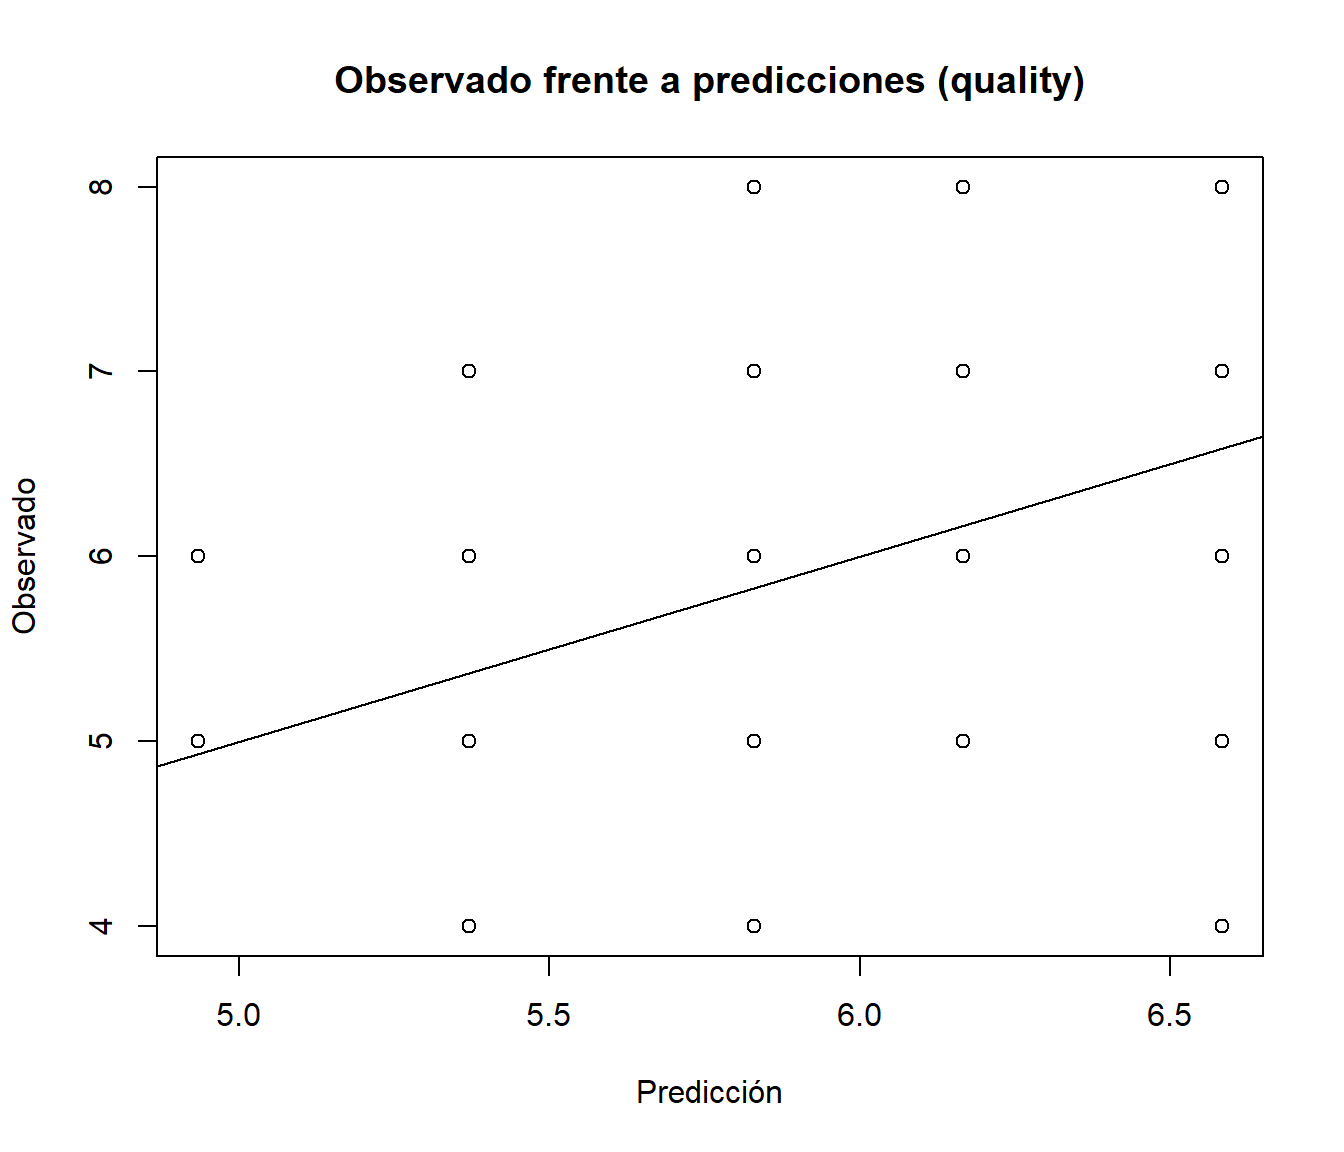
\includegraphics[width=0.8\linewidth]{02-arboles_files/figure-latex/unnamed-chunk-17-1} \end{center}

\begin{Shaded}
\begin{Highlighting}[]
\CommentTok{# Empleando el paquete caret }
\NormalTok{caret}\OperatorTok{::}\KeywordTok{postResample}\NormalTok{(pred, obs)}
\end{Highlighting}
\end{Shaded}

\begin{verbatim}
##      RMSE  Rsquared       MAE 
## 0.8145614 0.1969485 0.6574264
\end{verbatim}

\begin{Shaded}
\begin{Highlighting}[]
\CommentTok{# Con la función accuracy()}
\NormalTok{accuracy <-}\StringTok{ }\ControlFlowTok{function}\NormalTok{(pred, obs, }\DataTypeTok{na.rm =} \OtherTok{FALSE}\NormalTok{, }
                     \DataTypeTok{tol =} \KeywordTok{sqrt}\NormalTok{(.Machine}\OperatorTok{$}\NormalTok{double.eps)) \{}
\NormalTok{  err <-}\StringTok{ }\NormalTok{obs }\OperatorTok{-}\StringTok{ }\NormalTok{pred     }\CommentTok{# Errores}
  \ControlFlowTok{if}\NormalTok{(na.rm) \{}
\NormalTok{    is.a <-}\StringTok{ }\OperatorTok{!}\KeywordTok{is.na}\NormalTok{(err)}
\NormalTok{    err <-}\StringTok{ }\NormalTok{err[is.a]}
\NormalTok{    obs <-}\StringTok{ }\NormalTok{obs[is.a]}
\NormalTok{  \}  }
\NormalTok{  perr <-}\StringTok{ }\DecValTok{100}\OperatorTok{*}\NormalTok{err}\OperatorTok{/}\KeywordTok{pmax}\NormalTok{(obs, tol)  }\CommentTok{# Errores porcentuales}
  \KeywordTok{return}\NormalTok{(}\KeywordTok{c}\NormalTok{(}
    \DataTypeTok{me =} \KeywordTok{mean}\NormalTok{(err),           }\CommentTok{# Error medio}
    \DataTypeTok{rmse =} \KeywordTok{sqrt}\NormalTok{(}\KeywordTok{mean}\NormalTok{(err}\OperatorTok{^}\DecValTok{2}\NormalTok{)), }\CommentTok{# Raíz del error cuadrático medio }
    \DataTypeTok{mae =} \KeywordTok{mean}\NormalTok{(}\KeywordTok{abs}\NormalTok{(err)),     }\CommentTok{# Error absoluto medio}
    \DataTypeTok{mpe =} \KeywordTok{mean}\NormalTok{(perr),         }\CommentTok{# Error porcentual medio}
    \DataTypeTok{mape =} \KeywordTok{mean}\NormalTok{(}\KeywordTok{abs}\NormalTok{(perr)),   }\CommentTok{# Error porcentual absoluto medio}
    \DataTypeTok{r.squared =} \DecValTok{1} \OperatorTok{-}\StringTok{ }\KeywordTok{sum}\NormalTok{(err}\OperatorTok{^}\DecValTok{2}\NormalTok{)}\OperatorTok{/}\KeywordTok{sum}\NormalTok{((obs }\OperatorTok{-}\StringTok{ }\KeywordTok{mean}\NormalTok{(obs))}\OperatorTok{^}\DecValTok{2}\NormalTok{)}
\NormalTok{  ))}
\NormalTok{\}}
\KeywordTok{accuracy}\NormalTok{(pred, test}\OperatorTok{$}\NormalTok{quality)}
\end{Highlighting}
\end{Shaded}

\begin{verbatim}
##           me         rmse          mae          mpe         mape    r.squared 
## -0.001269398  0.814561435  0.657426365 -1.952342173 11.576716037  0.192007721
\end{verbatim}

\subsection{Ejemplo: modelo de clasificación}\label{class-rpart}

Para ilustrar los árboles de clasificación CART, podemos emplear los
datos anteriores de calidad de vino, considerando como respuesta una
nueva variable \texttt{taste} que clasifica los vinos en ``good'' o
``bad'' dependiendo de si
\texttt{winequality\$quality\ \textgreater{}=\ 5} (este conjunto de
datos está almacenado en el archivo \emph{winetaste.RData}).

\begin{Shaded}
\begin{Highlighting}[]
\CommentTok{# load("data/winetaste.RData")}
\NormalTok{winetaste <-}\StringTok{ }\NormalTok{winequality[, }\KeywordTok{colnames}\NormalTok{(winequality)}\OperatorTok{!=}\StringTok{"quality"}\NormalTok{]}
\NormalTok{winetaste}\OperatorTok{$}\NormalTok{taste <-}\StringTok{ }\KeywordTok{factor}\NormalTok{(winequality}\OperatorTok{$}\NormalTok{quality }\OperatorTok{<}\StringTok{ }\DecValTok{6}\NormalTok{, }\DataTypeTok{labels =} \KeywordTok{c}\NormalTok{(}\StringTok{'good'}\NormalTok{, }\StringTok{'bad'}\NormalTok{)) }\CommentTok{# levels = c('FALSE', 'TRUE')}
\KeywordTok{str}\NormalTok{(winetaste)}
\end{Highlighting}
\end{Shaded}

\begin{verbatim}
## 'data.frame':    1250 obs. of  12 variables:
##  $ fixed.acidity       : num  6.8 7.1 6.9 7.5 8.6 7.7 5.4 6.8 6.1 5.5 ...
##  $ volatile.acidity    : num  0.37 0.24 0.32 0.23 0.36 0.28 0.59 0.16 0.28 0.28 ...
##  $ citric.acid         : num  0.47 0.34 0.13 0.49 0.26 0.63 0.07 0.36 0.27 0.21 ...
##  $ residual.sugar      : num  11.2 1.2 7.8 7.7 11.1 11.1 7 1.3 4.7 1.6 ...
##  $ chlorides           : num  0.071 0.045 0.042 0.049 0.03 0.039 0.045 0.034 0.03 0.032 ...
##  $ free.sulfur.dioxide : num  44 6 11 61 43.5 58 36 32 56 23 ...
##  $ total.sulfur.dioxide: num  136 132 117 209 171 179 147 98 140 85 ...
##  $ density             : num  0.997 0.991 0.996 0.994 0.995 ...
##  $ pH                  : num  2.98 3.16 3.23 3.14 3.03 3.08 3.34 3.02 3.16 3.42 ...
##  $ sulphates           : num  0.88 0.46 0.37 0.3 0.49 0.44 0.57 0.58 0.42 0.42 ...
##  $ alcohol             : num  9.2 11.2 9.2 11.1 12 8.8 9.7 11.3 12.5 12.5 ...
##  $ taste               : Factor w/ 2 levels "good","bad": 2 2 2 1 2 2 1 1 1 2 ...
\end{verbatim}

\begin{Shaded}
\begin{Highlighting}[]
\KeywordTok{table}\NormalTok{(winetaste}\OperatorTok{$}\NormalTok{taste)}
\end{Highlighting}
\end{Shaded}

\begin{verbatim}
## 
## good  bad 
##  828  422
\end{verbatim}

Como en el caso anterior, se contruyen las muestras de entrenamiento
(80\%) y de test (20\%):

\begin{Shaded}
\begin{Highlighting}[]
\CommentTok{# set.seed(1)}
\CommentTok{# nobs <- nrow(winetaste)}
\CommentTok{# itrain <- sample(nobs, 0.8 * nobs)}
\NormalTok{train <-}\StringTok{ }\NormalTok{winetaste[itrain, ]}
\NormalTok{test <-}\StringTok{ }\NormalTok{winetaste[}\OperatorTok{-}\NormalTok{itrain, ]}
\end{Highlighting}
\end{Shaded}

Al igual que en el caso anterior podemos obtener el árbol de
clasificación con las opciones por defecto (\texttt{cp\ =\ 0.01} y
\texttt{split\ =\ "gini"}) con el comando:

\begin{Shaded}
\begin{Highlighting}[]
\NormalTok{tree <-}\StringTok{ }\KeywordTok{rpart}\NormalTok{(taste }\OperatorTok{~}\StringTok{ }\NormalTok{., }\DataTypeTok{data =}\NormalTok{ train)}
\end{Highlighting}
\end{Shaded}

En este caso al imprimirlo como información de los nodos se muestra
(además del número de nodo, la condición de la partición y el número de
observaciones en el nodo) el número de observaciones mal clasificadas,
la predicción y las proporciones estimadas (frecuencias relativas en la
muestra de entrenamiento) de las clases:

\begin{Shaded}
\begin{Highlighting}[]
\NormalTok{tree}
\end{Highlighting}
\end{Shaded}

\begin{verbatim}
## n= 1000 
## 
## node), split, n, loss, yval, (yprob)
##       * denotes terminal node
## 
##  1) root 1000 338 good (0.6620000 0.3380000)  
##    2) alcohol>=10.11667 541 100 good (0.8151571 0.1848429)  
##      4) free.sulfur.dioxide>=8.5 522  87 good (0.8333333 0.1666667)  
##        8) fixed.acidity< 8.55 500  73 good (0.8540000 0.1460000) *
##        9) fixed.acidity>=8.55 22   8 bad (0.3636364 0.6363636) *
##      5) free.sulfur.dioxide< 8.5 19   6 bad (0.3157895 0.6842105) *
##    3) alcohol< 10.11667 459 221 bad (0.4814815 0.5185185)  
##      6) volatile.acidity< 0.2875 264 102 good (0.6136364 0.3863636)  
##       12) fixed.acidity< 7.45 213  71 good (0.6666667 0.3333333)  
##         24) citric.acid>=0.265 160  42 good (0.7375000 0.2625000) *
##         25) citric.acid< 0.265 53  24 bad (0.4528302 0.5471698)  
##           50) free.sulfur.dioxide< 42.5 33  13 good (0.6060606 0.3939394) *
##           51) free.sulfur.dioxide>=42.5 20   4 bad (0.2000000 0.8000000) *
##       13) fixed.acidity>=7.45 51  20 bad (0.3921569 0.6078431)  
##         26) total.sulfur.dioxide>=150 26  10 good (0.6153846 0.3846154) *
##         27) total.sulfur.dioxide< 150 25   4 bad (0.1600000 0.8400000) *
##      7) volatile.acidity>=0.2875 195  59 bad (0.3025641 0.6974359)  
##       14) pH>=3.235 49  24 bad (0.4897959 0.5102041)  
##         28) chlorides< 0.0465 18   4 good (0.7777778 0.2222222) *
##         29) chlorides>=0.0465 31  10 bad (0.3225806 0.6774194) *
##       15) pH< 3.235 146  35 bad (0.2397260 0.7602740) *
\end{verbatim}

También puede ser preferible emplear el paquete
\href{https://CRAN.R-project.org/package=rpart.plot}{\texttt{rpart.plot}}
para representarlo:

\begin{Shaded}
\begin{Highlighting}[]
\KeywordTok{library}\NormalTok{(rpart.plot)}
\KeywordTok{rpart.plot}\NormalTok{(tree, }\DataTypeTok{main=}\StringTok{"Classification tree winetaste"}\NormalTok{) }\CommentTok{# Alternativa: rattle::fancyRpartPlot}
\end{Highlighting}
\end{Shaded}

\begin{center}\includegraphics[width=0.8\linewidth]{02-arboles_files/figure-latex/unnamed-chunk-22-1} \end{center}

\begin{Shaded}
\begin{Highlighting}[]
\KeywordTok{rpart.plot}\NormalTok{(tree, }\DataTypeTok{main=}\StringTok{"Classification tree winetaste"}\NormalTok{,}
           \DataTypeTok{extra =} \DecValTok{104}\NormalTok{,          }\CommentTok{# show fitted class, probs, percentages}
           \DataTypeTok{box.palette =} \StringTok{"GnBu"}\NormalTok{, }\CommentTok{# color scheme}
           \DataTypeTok{branch.lty =} \DecValTok{3}\NormalTok{,       }\CommentTok{# dotted branch lines}
           \DataTypeTok{shadow.col =} \StringTok{"gray"}\NormalTok{,  }\CommentTok{# shadows under the node boxes}
           \DataTypeTok{nn =} \OtherTok{TRUE}\NormalTok{)            }\CommentTok{# display the node numbers }
\end{Highlighting}
\end{Shaded}

\begin{center}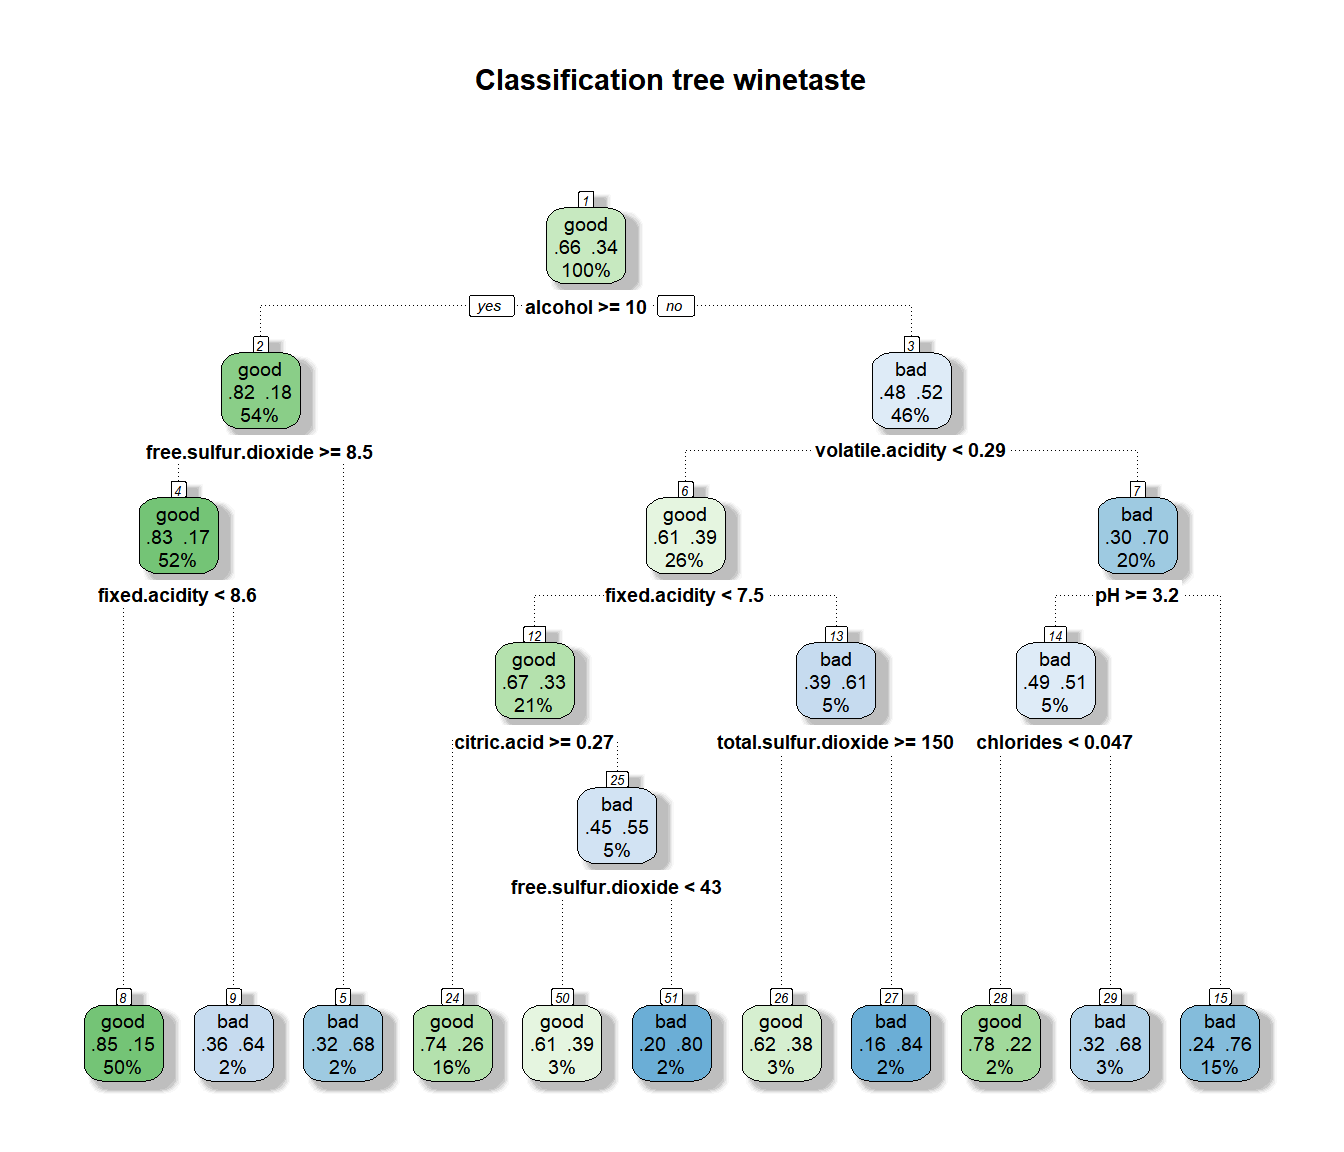
\includegraphics[width=0.8\linewidth]{02-arboles_files/figure-latex/unnamed-chunk-22-2} \end{center}

Nos interesa como se clasificaría a una nueva observación (como se llega
a los nodos terminales) y su probabilidad estimada (la frecuencia
relativa de la clase más frecuente en el correspondiente nodo terminal).
Al igual que en el caso de regresión, puede ser de utilidad imprimir las
reglas:

\begin{Shaded}
\begin{Highlighting}[]
\KeywordTok{rpart.rules}\NormalTok{(tree, }\DataTypeTok{style =} \StringTok{"tall"}\NormalTok{)}
\end{Highlighting}
\end{Shaded}

\begin{verbatim}
## taste is 0.15 when
##     alcohol >= 10
##     fixed.acidity < 8.6
##     free.sulfur.dioxide >= 8.5
## 
## taste is 0.22 when
##     alcohol < 10
##     volatile.acidity >= 0.29
##     pH >= 3.2
##     chlorides < 0.047
## 
## taste is 0.26 when
##     alcohol < 10
##     volatile.acidity < 0.29
##     fixed.acidity < 7.5
##     citric.acid >= 0.27
## 
## taste is 0.38 when
##     alcohol < 10
##     volatile.acidity < 0.29
##     fixed.acidity >= 7.5
##     total.sulfur.dioxide >= 150
## 
## taste is 0.39 when
##     alcohol < 10
##     volatile.acidity < 0.29
##     fixed.acidity < 7.5
##     free.sulfur.dioxide < 42.5
##     citric.acid < 0.27
## 
## taste is 0.64 when
##     alcohol >= 10
##     fixed.acidity >= 8.6
##     free.sulfur.dioxide >= 8.5
## 
## taste is 0.68 when
##     alcohol < 10
##     volatile.acidity >= 0.29
##     pH >= 3.2
##     chlorides >= 0.047
## 
## taste is 0.68 when
##     alcohol >= 10
##     free.sulfur.dioxide < 8.5
## 
## taste is 0.76 when
##     alcohol < 10
##     volatile.acidity >= 0.29
##     pH < 3.2
## 
## taste is 0.80 when
##     alcohol < 10
##     volatile.acidity < 0.29
##     fixed.acidity < 7.5
##     free.sulfur.dioxide >= 42.5
##     citric.acid < 0.27
## 
## taste is 0.84 when
##     alcohol < 10
##     volatile.acidity < 0.29
##     fixed.acidity >= 7.5
##     total.sulfur.dioxide < 150
\end{verbatim}

Al igual que en el caso anterior, para seleccionar un valor óptimo del
(hiper)parámetro de complejidad, se puede construir un árbol de decisión
completo y emplear validación cruzada para podarlo. Además, si el número
de observaciones es grande y las clases están más o menos balanceadas,
se podría aumentar los valores mínimos de observaciones en los nodos
intermedios y terminales\footnote{Otra opción, más interesante para
  regresión, sería considerar estos valores como hiperparámetros.}, por
ejemplo:

\begin{Shaded}
\begin{Highlighting}[]
\NormalTok{tree <-}\StringTok{ }\KeywordTok{rpart}\NormalTok{(taste }\OperatorTok{~}\StringTok{ }\NormalTok{., }\DataTypeTok{data =}\NormalTok{ train, }\DataTypeTok{cp =} \DecValTok{0}\NormalTok{, }\DataTypeTok{minsplit =} \DecValTok{30}\NormalTok{, }\DataTypeTok{minbucket =} \DecValTok{10}\NormalTok{)}
\end{Highlighting}
\end{Shaded}

En este caso mantenemos el resto de valores por defecto:

\begin{Shaded}
\begin{Highlighting}[]
\NormalTok{tree <-}\StringTok{ }\KeywordTok{rpart}\NormalTok{(taste }\OperatorTok{~}\StringTok{ }\NormalTok{., }\DataTypeTok{data =}\NormalTok{ train, }\DataTypeTok{cp =} \DecValTok{0}\NormalTok{)}
\end{Highlighting}
\end{Shaded}

Representamos los errores (reescalados) de validación cruzada:

\begin{Shaded}
\begin{Highlighting}[]
\CommentTok{# printcp(tree)}
\KeywordTok{plotcp}\NormalTok{(tree)}
\end{Highlighting}
\end{Shaded}

\begin{center}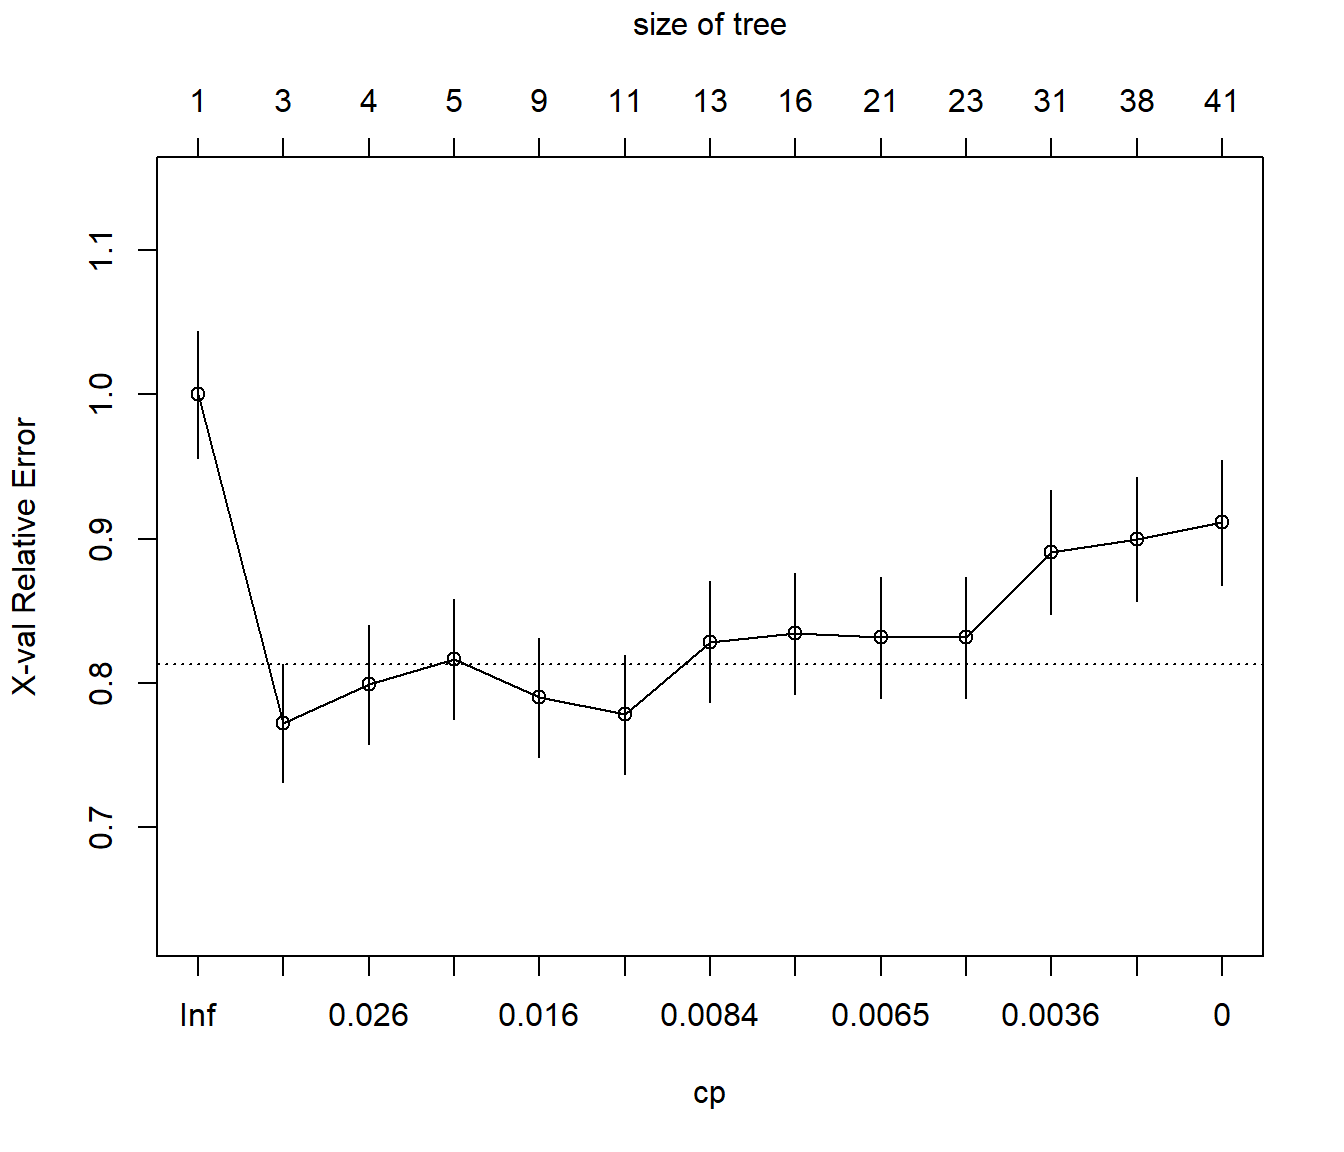
\includegraphics[width=0.8\linewidth]{02-arboles_files/figure-latex/unnamed-chunk-26-1} \end{center}

Para obtener el modelo final, seleccionamos el valor óptimo de
complejidad siguiendo el criterio de un error estándar de Breiman et al.
(1984) y podamos el arbol:

\begin{Shaded}
\begin{Highlighting}[]
\NormalTok{xerror <-}\StringTok{ }\NormalTok{tree}\OperatorTok{$}\NormalTok{cptable[,}\StringTok{"xerror"}\NormalTok{]}
\NormalTok{imin.xerror <-}\StringTok{ }\KeywordTok{which.min}\NormalTok{(xerror)}
\NormalTok{upper.xerror <-}\StringTok{ }\NormalTok{xerror[imin.xerror] }\OperatorTok{+}\StringTok{ }\NormalTok{tree}\OperatorTok{$}\NormalTok{cptable[imin.xerror, }\StringTok{"xstd"}\NormalTok{]}
\NormalTok{icp <-}\StringTok{ }\KeywordTok{min}\NormalTok{(}\KeywordTok{which}\NormalTok{(xerror }\OperatorTok{<=}\StringTok{ }\NormalTok{upper.xerror))}
\NormalTok{cp <-}\StringTok{ }\NormalTok{tree}\OperatorTok{$}\NormalTok{cptable[icp, }\StringTok{"CP"}\NormalTok{]}
\NormalTok{tree <-}\StringTok{ }\KeywordTok{prune}\NormalTok{(tree, }\DataTypeTok{cp =}\NormalTok{ cp)}
\CommentTok{# tree}
\CommentTok{# summary(tree)}
\CommentTok{# caret::varImp(tree)}
\CommentTok{# importance <- tree$variable.importance}
\CommentTok{# importance <- round(100*importance/sum(importance), 1)}
\CommentTok{# importance[importance >= 1]}
\KeywordTok{rpart.plot}\NormalTok{(tree, }\DataTypeTok{main=}\StringTok{"Classification tree winetaste"}\NormalTok{)}
\end{Highlighting}
\end{Shaded}

\begin{center}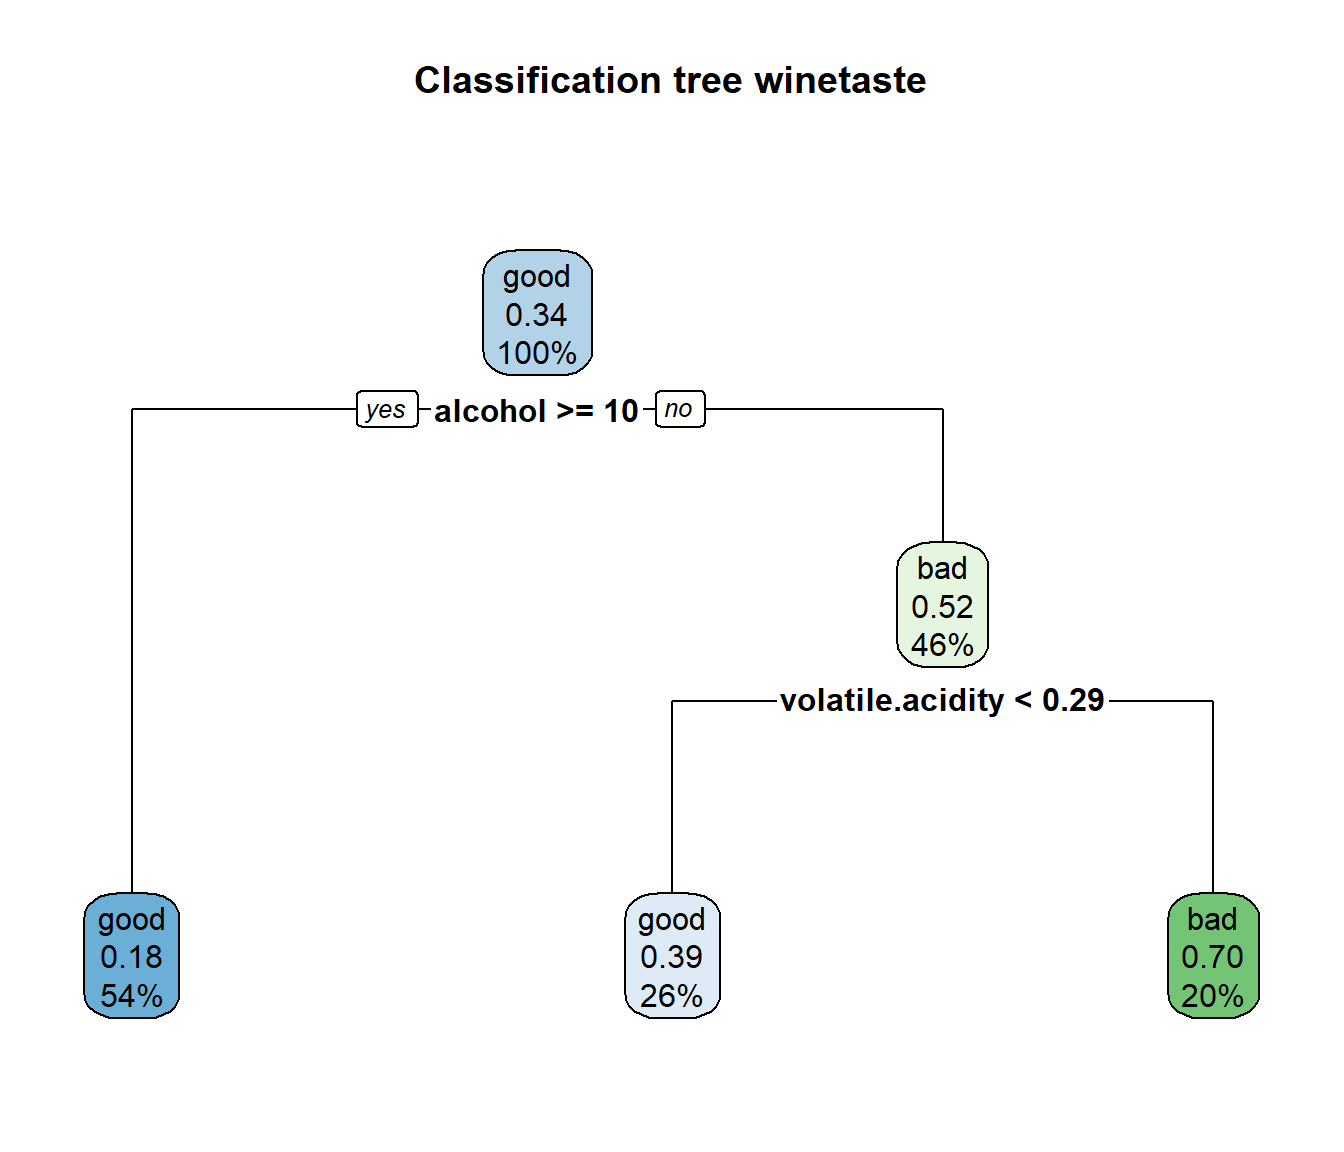
\includegraphics[width=0.8\linewidth]{02-arboles_files/figure-latex/unnamed-chunk-27-1} \end{center}

El último paso sería evaluarlo en la muestra de test siguiendo los pasos
descritos en la Sección \ref{eval-class}. El método \texttt{predict()}
por defecto (\texttt{type\ =\ "prob"}) devuelve una matriz con las
probabilidades de cada clase, habrá que establecer
\texttt{type\ =\ "class"} (para más detalles consultar la ayuda de
\texttt{predic.rpart()}).

\begin{Shaded}
\begin{Highlighting}[]
\NormalTok{obs <-}\StringTok{ }\NormalTok{test}\OperatorTok{$}\NormalTok{taste}
\KeywordTok{head}\NormalTok{(}\KeywordTok{predict}\NormalTok{(tree, }\DataTypeTok{newdata =}\NormalTok{ test))}
\end{Highlighting}
\end{Shaded}

\begin{verbatim}
##         good       bad
## 1  0.3025641 0.6974359
## 4  0.8151571 0.1848429
## 9  0.8151571 0.1848429
## 10 0.8151571 0.1848429
## 12 0.8151571 0.1848429
## 16 0.8151571 0.1848429
\end{verbatim}

\begin{Shaded}
\begin{Highlighting}[]
\NormalTok{pred <-}\StringTok{ }\KeywordTok{predict}\NormalTok{(tree, }\DataTypeTok{newdata =}\NormalTok{ test, }\DataTypeTok{type =} \StringTok{"class"}\NormalTok{)}
\KeywordTok{table}\NormalTok{(obs, pred)}
\end{Highlighting}
\end{Shaded}

\begin{verbatim}
##       pred
## obs    good bad
##   good  153  13
##   bad    54  30
\end{verbatim}

\begin{Shaded}
\begin{Highlighting}[]
\NormalTok{caret}\OperatorTok{::}\KeywordTok{confusionMatrix}\NormalTok{(pred, obs)}
\end{Highlighting}
\end{Shaded}

\begin{verbatim}
## Confusion Matrix and Statistics
## 
##           Reference
## Prediction good bad
##       good  153  54
##       bad    13  30
##                                           
##                Accuracy : 0.732           
##                  95% CI : (0.6725, 0.7859)
##     No Information Rate : 0.664           
##     P-Value [Acc > NIR] : 0.01247         
##                                           
##                   Kappa : 0.3171          
##                                           
##  Mcnemar's Test P-Value : 1.025e-06       
##                                           
##             Sensitivity : 0.9217          
##             Specificity : 0.3571          
##          Pos Pred Value : 0.7391          
##          Neg Pred Value : 0.6977          
##              Prevalence : 0.6640          
##          Detection Rate : 0.6120          
##    Detection Prevalence : 0.8280          
##       Balanced Accuracy : 0.6394          
##                                           
##        'Positive' Class : good            
## 
\end{verbatim}

\subsection{\texorpdfstring{Interfaz de
\texttt{caret}}{Interfaz de caret}}\label{interfaz-de-caret}

En \texttt{caret} podemos ajustar un árbol CART seleccionando
\texttt{method\ =\ "rpart"}. Por defecto emplea bootstrap de las
observaciones para seleccionar el valor óptimo del hiperparámetro
\texttt{cp} (considerando únicamente tres posibles valores). Si queremos
emplear validación cruzada como en el caso anterior podemos emplear la
función auxiliar \texttt{trainControl()} y para considerar un mayor
rango de posibles valores, el argumento \texttt{tuneLength}.

\begin{Shaded}
\begin{Highlighting}[]
\KeywordTok{library}\NormalTok{(caret)}
\CommentTok{# names(getModelInfo()) # Listado de todos los métodos disponibles}
\CommentTok{# modelLookup("rpart")  # Información sobre hiperparámetros}
\KeywordTok{set.seed}\NormalTok{(}\DecValTok{1}\NormalTok{)}
\CommentTok{# itrain <- <- createDataPartition(winetaste$taste, p = 0.8, list = FALSE)}
\CommentTok{# train <- winetaste[itrain, ]}
\CommentTok{# test <- winetaste[-itrain, ]}
\NormalTok{caret.rpart <-}\StringTok{ }\KeywordTok{train}\NormalTok{(taste }\OperatorTok{~}\StringTok{ }\NormalTok{., }\DataTypeTok{method =} \StringTok{"rpart"}\NormalTok{, }\DataTypeTok{data =}\NormalTok{ train, }
                     \DataTypeTok{tuneLength =} \DecValTok{20}\NormalTok{,}
                     \DataTypeTok{trControl =} \KeywordTok{trainControl}\NormalTok{(}\DataTypeTok{method =} \StringTok{"cv"}\NormalTok{, }\DataTypeTok{number =} \DecValTok{10}\NormalTok{)) }
\NormalTok{caret.rpart}
\end{Highlighting}
\end{Shaded}

\begin{verbatim}
## CART 
## 
## 1000 samples
##   11 predictor
##    2 classes: 'good', 'bad' 
## 
## No pre-processing
## Resampling: Cross-Validated (10 fold) 
## Summary of sample sizes: 901, 900, 900, 900, 900, 900, ... 
## Resampling results across tuning parameters:
## 
##   cp           Accuracy   Kappa    
##   0.000000000  0.7018843  0.3487338
##   0.005995017  0.7330356  0.3870552
##   0.011990034  0.7410655  0.3878517
##   0.017985051  0.7230748  0.3374518
##   0.023980069  0.7360748  0.3698691
##   0.029975086  0.7340748  0.3506377
##   0.035970103  0.7320748  0.3418235
##   0.041965120  0.7350849  0.3422651
##   0.047960137  0.7350849  0.3422651
##   0.053955154  0.7350849  0.3422651
##   0.059950171  0.7350849  0.3422651
##   0.065945188  0.7350849  0.3422651
##   0.071940206  0.7350849  0.3422651
##   0.077935223  0.7350849  0.3422651
##   0.083930240  0.7350849  0.3422651
##   0.089925257  0.7350849  0.3422651
##   0.095920274  0.7350849  0.3422651
##   0.101915291  0.7350849  0.3422651
##   0.107910308  0.7229637  0.2943312
##   0.113905325  0.6809637  0.1087694
## 
## Accuracy was used to select the optimal model using the largest value.
## The final value used for the model was cp = 0.01199003.
\end{verbatim}

\begin{Shaded}
\begin{Highlighting}[]
\KeywordTok{ggplot}\NormalTok{(caret.rpart)}
\end{Highlighting}
\end{Shaded}

\begin{center}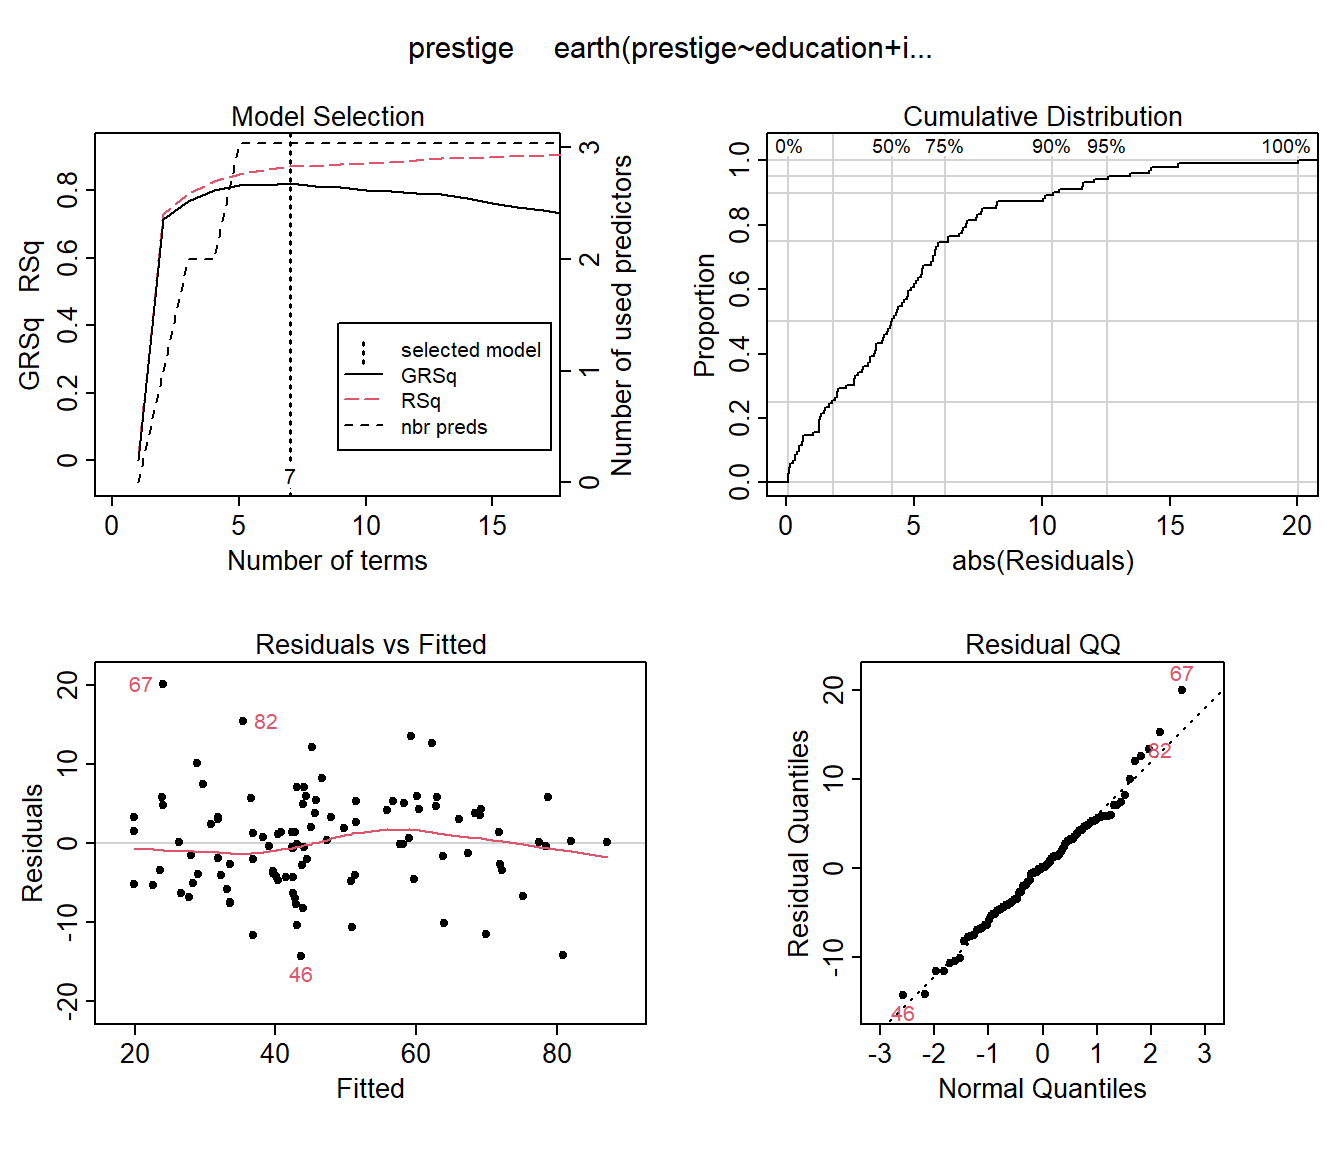
\includegraphics[width=0.8\linewidth]{02-arboles_files/figure-latex/unnamed-chunk-29-1} \end{center}

\begin{Shaded}
\begin{Highlighting}[]
\NormalTok{caret.rpart}\OperatorTok{$}\NormalTok{finalModel}
\end{Highlighting}
\end{Shaded}

\begin{verbatim}
## n= 1000 
## 
## node), split, n, loss, yval, (yprob)
##       * denotes terminal node
## 
##  1) root 1000 338 good (0.6620000 0.3380000)  
##    2) alcohol>=10.11667 541 100 good (0.8151571 0.1848429)  
##      4) free.sulfur.dioxide>=8.5 522  87 good (0.8333333 0.1666667)  
##        8) fixed.acidity< 8.55 500  73 good (0.8540000 0.1460000) *
##        9) fixed.acidity>=8.55 22   8 bad (0.3636364 0.6363636) *
##      5) free.sulfur.dioxide< 8.5 19   6 bad (0.3157895 0.6842105) *
##    3) alcohol< 10.11667 459 221 bad (0.4814815 0.5185185)  
##      6) volatile.acidity< 0.2875 264 102 good (0.6136364 0.3863636)  
##       12) fixed.acidity< 7.45 213  71 good (0.6666667 0.3333333)  
##         24) citric.acid>=0.265 160  42 good (0.7375000 0.2625000) *
##         25) citric.acid< 0.265 53  24 bad (0.4528302 0.5471698)  
##           50) free.sulfur.dioxide< 42.5 33  13 good (0.6060606 0.3939394) *
##           51) free.sulfur.dioxide>=42.5 20   4 bad (0.2000000 0.8000000) *
##       13) fixed.acidity>=7.45 51  20 bad (0.3921569 0.6078431)  
##         26) total.sulfur.dioxide>=150 26  10 good (0.6153846 0.3846154) *
##         27) total.sulfur.dioxide< 150 25   4 bad (0.1600000 0.8400000) *
##      7) volatile.acidity>=0.2875 195  59 bad (0.3025641 0.6974359)  
##       14) pH>=3.235 49  24 bad (0.4897959 0.5102041)  
##         28) chlorides< 0.0465 18   4 good (0.7777778 0.2222222) *
##         29) chlorides>=0.0465 31  10 bad (0.3225806 0.6774194) *
##       15) pH< 3.235 146  35 bad (0.2397260 0.7602740) *
\end{verbatim}

\begin{Shaded}
\begin{Highlighting}[]
\KeywordTok{rpart.plot}\NormalTok{(caret.rpart}\OperatorTok{$}\NormalTok{finalModel, }\DataTypeTok{main=}\StringTok{"Classification tree winetaste"}\NormalTok{)}
\end{Highlighting}
\end{Shaded}

\begin{center}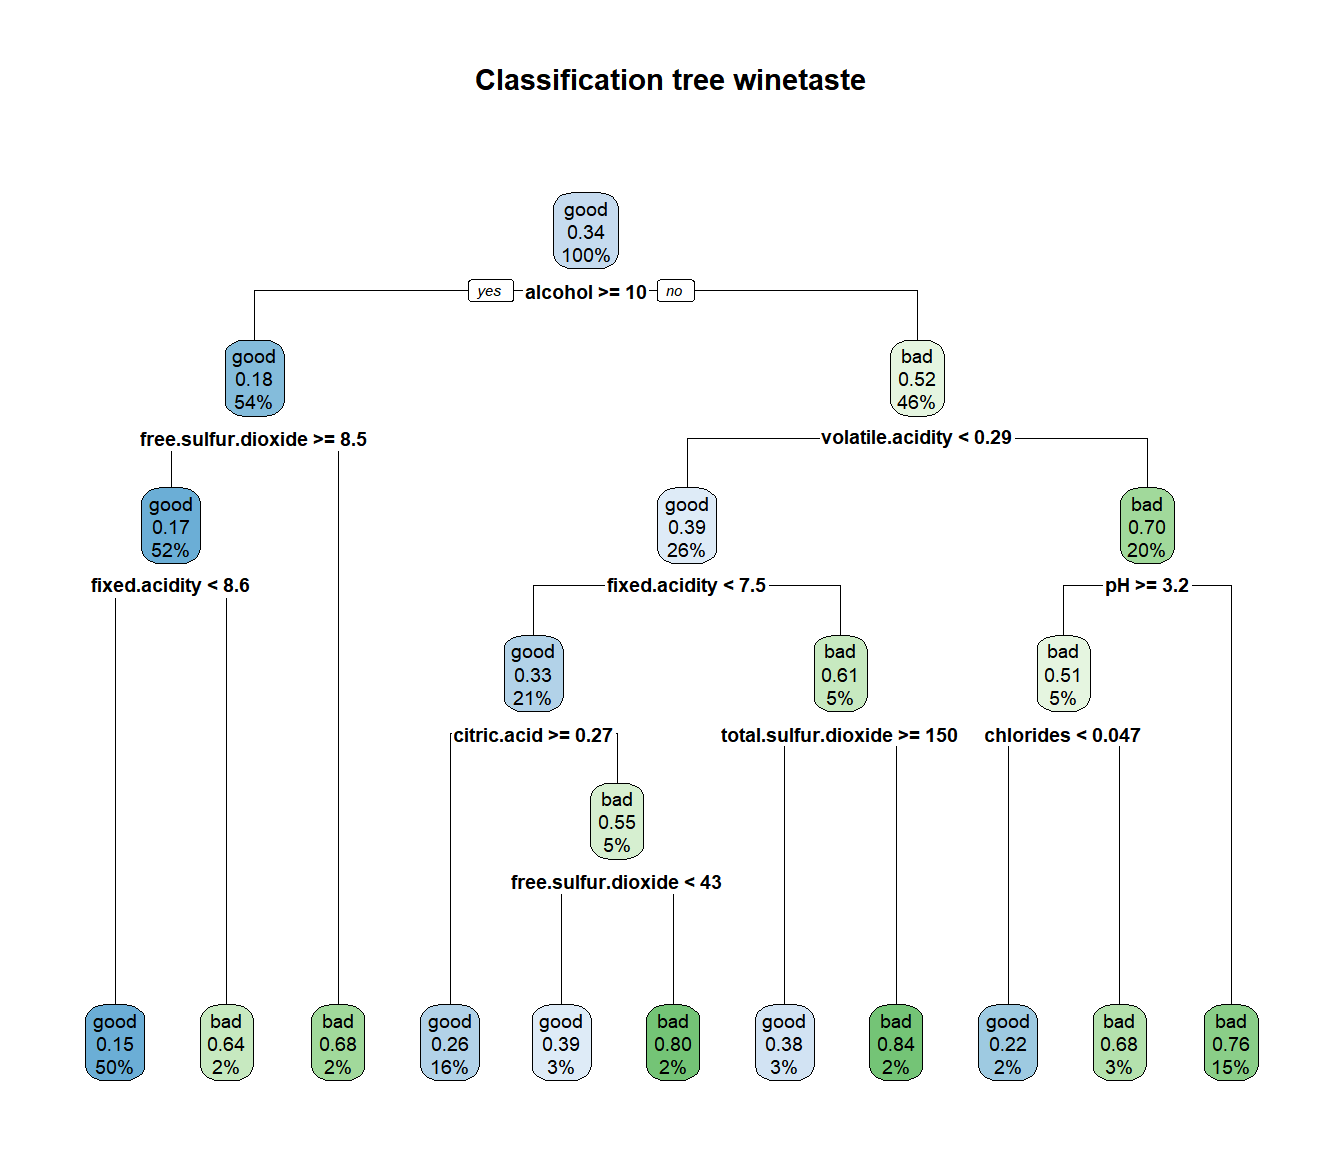
\includegraphics[width=0.8\linewidth]{02-arboles_files/figure-latex/unnamed-chunk-29-2} \end{center}

Para utilizar la regla de ``un error estándar'' se puede añadir
\texttt{selectionFunction\ =\ "oneSE"}

\begin{Shaded}
\begin{Highlighting}[]
\KeywordTok{set.seed}\NormalTok{(}\DecValTok{1}\NormalTok{)}
\NormalTok{caret.rpart <-}\StringTok{ }\KeywordTok{train}\NormalTok{(taste }\OperatorTok{~}\StringTok{ }\NormalTok{., }\DataTypeTok{method =} \StringTok{"rpart"}\NormalTok{, }\DataTypeTok{data =}\NormalTok{ train, }
                     \DataTypeTok{tuneLength =} \DecValTok{20}\NormalTok{,}
                     \DataTypeTok{trControl =} \KeywordTok{trainControl}\NormalTok{(}\DataTypeTok{method =} \StringTok{"cv"}\NormalTok{, }\DataTypeTok{number =} \DecValTok{10}\NormalTok{,}
                                              \DataTypeTok{selectionFunction =} \StringTok{"oneSE"}\NormalTok{)) }
\NormalTok{caret.rpart}
\end{Highlighting}
\end{Shaded}

\begin{verbatim}
## CART 
## 
## 1000 samples
##   11 predictor
##    2 classes: 'good', 'bad' 
## 
## No pre-processing
## Resampling: Cross-Validated (10 fold) 
## Summary of sample sizes: 901, 900, 900, 900, 900, 900, ... 
## Resampling results across tuning parameters:
## 
##   cp           Accuracy   Kappa    
##   0.000000000  0.7018843  0.3487338
##   0.005995017  0.7330356  0.3870552
##   0.011990034  0.7410655  0.3878517
##   0.017985051  0.7230748  0.3374518
##   0.023980069  0.7360748  0.3698691
##   0.029975086  0.7340748  0.3506377
##   0.035970103  0.7320748  0.3418235
##   0.041965120  0.7350849  0.3422651
##   0.047960137  0.7350849  0.3422651
##   0.053955154  0.7350849  0.3422651
##   0.059950171  0.7350849  0.3422651
##   0.065945188  0.7350849  0.3422651
##   0.071940206  0.7350849  0.3422651
##   0.077935223  0.7350849  0.3422651
##   0.083930240  0.7350849  0.3422651
##   0.089925257  0.7350849  0.3422651
##   0.095920274  0.7350849  0.3422651
##   0.101915291  0.7350849  0.3422651
##   0.107910308  0.7229637  0.2943312
##   0.113905325  0.6809637  0.1087694
## 
## Accuracy was used to select the optimal model using  the one SE rule.
## The final value used for the model was cp = 0.1019153.
\end{verbatim}

\begin{Shaded}
\begin{Highlighting}[]
\CommentTok{# ggplot(caret.rpart)}
\NormalTok{caret.rpart}\OperatorTok{$}\NormalTok{finalModel}
\end{Highlighting}
\end{Shaded}

\begin{verbatim}
## n= 1000 
## 
## node), split, n, loss, yval, (yprob)
##       * denotes terminal node
## 
## 1) root 1000 338 good (0.6620000 0.3380000)  
##   2) alcohol>=10.11667 541 100 good (0.8151571 0.1848429) *
##   3) alcohol< 10.11667 459 221 bad (0.4814815 0.5185185)  
##     6) volatile.acidity< 0.2875 264 102 good (0.6136364 0.3863636) *
##     7) volatile.acidity>=0.2875 195  59 bad (0.3025641 0.6974359) *
\end{verbatim}

\begin{Shaded}
\begin{Highlighting}[]
\KeywordTok{rpart.plot}\NormalTok{(caret.rpart}\OperatorTok{$}\NormalTok{finalModel, }\DataTypeTok{main =} \StringTok{"Classification tree winetaste"}\NormalTok{)}
\end{Highlighting}
\end{Shaded}

\begin{center}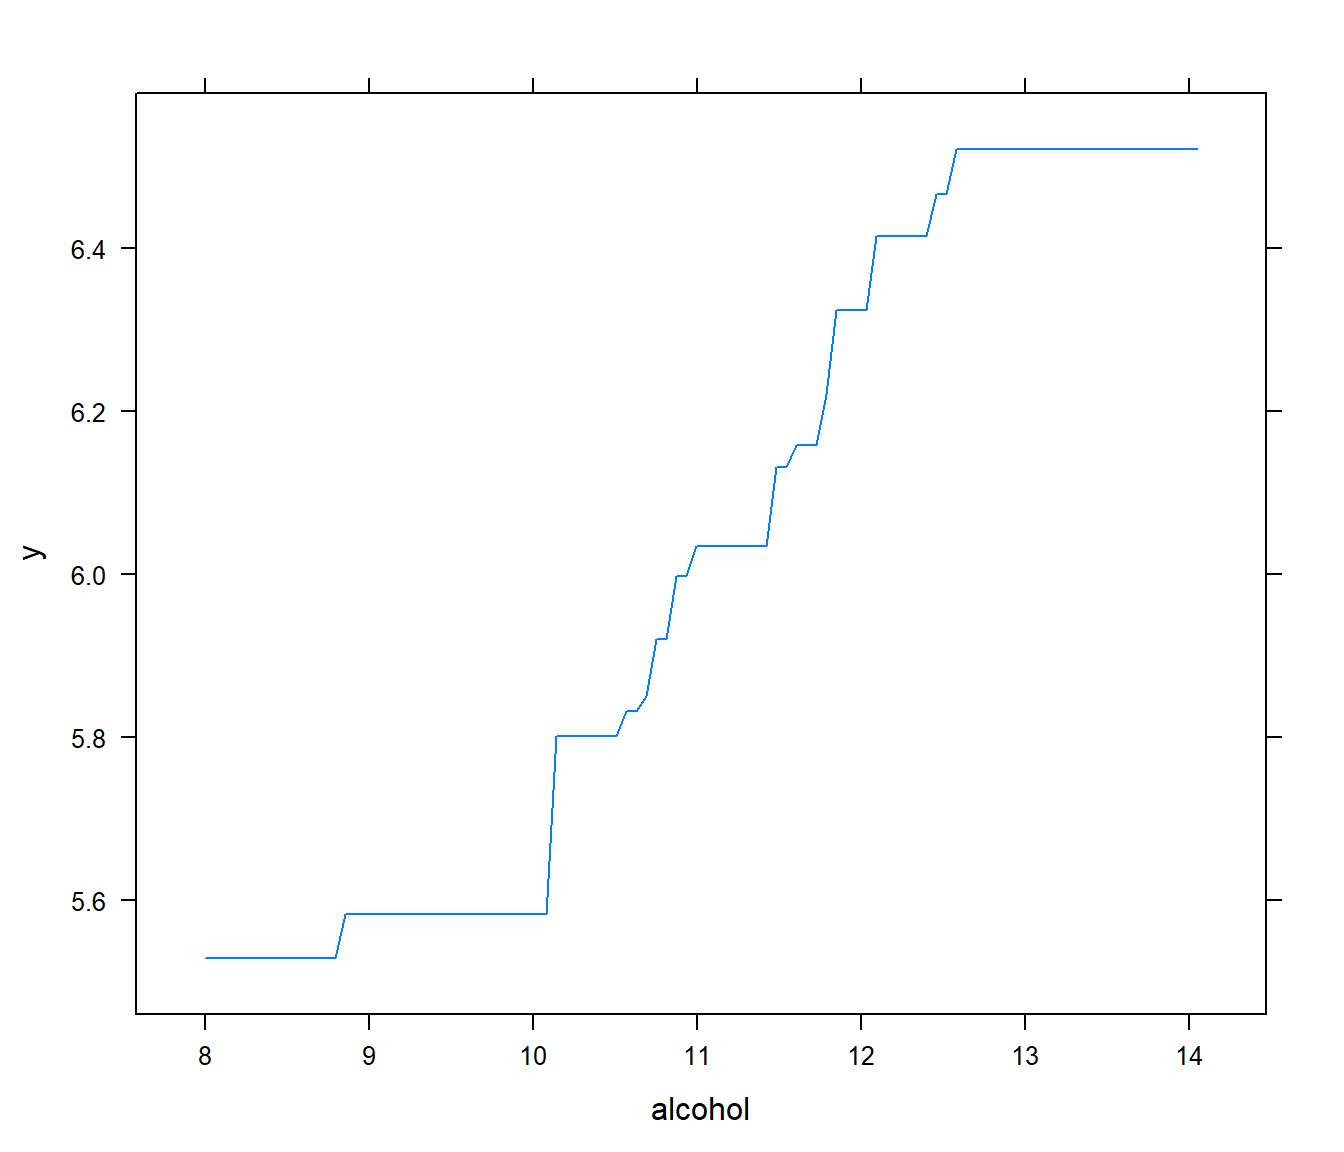
\includegraphics[width=0.8\linewidth]{02-arboles_files/figure-latex/unnamed-chunk-30-1} \end{center}

\begin{Shaded}
\begin{Highlighting}[]
\NormalTok{var.imp <-}\StringTok{ }\KeywordTok{varImp}\NormalTok{(caret.rpart)}
\KeywordTok{plot}\NormalTok{(var.imp)}
\end{Highlighting}
\end{Shaded}

\begin{center}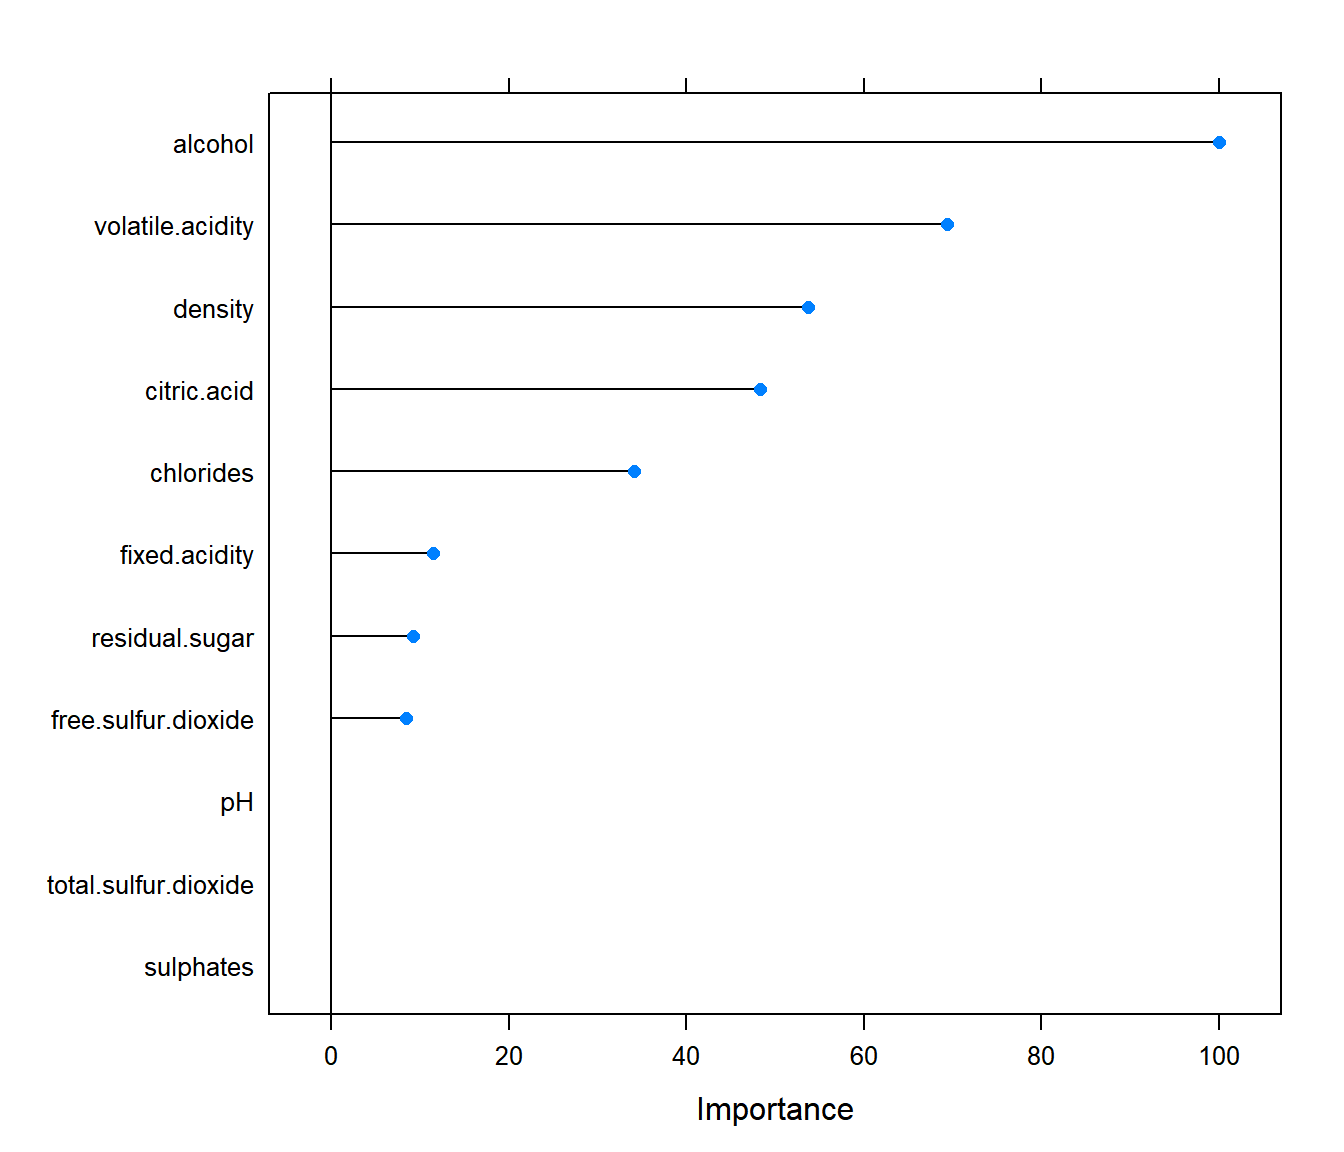
\includegraphics[width=0.8\linewidth]{02-arboles_files/figure-latex/unnamed-chunk-30-2} \end{center}

Para calcular las predicciones (o las estimaciones de las
probabilidades) podemos emplear el método \texttt{predict.train()} y
posteriormente \texttt{confusionMatrix()} para evaluar su precisión:

\begin{Shaded}
\begin{Highlighting}[]
\NormalTok{pred <-}\StringTok{ }\KeywordTok{predict}\NormalTok{(caret.rpart, }\DataTypeTok{newdata =}\NormalTok{ test)}
\CommentTok{# p.est <- predict(caret.rpart, newdata = test, type = "prob")}
\KeywordTok{confusionMatrix}\NormalTok{(pred, test}\OperatorTok{$}\NormalTok{taste)}
\end{Highlighting}
\end{Shaded}

\begin{verbatim}
## Confusion Matrix and Statistics
## 
##           Reference
## Prediction good bad
##       good  153  54
##       bad    13  30
##                                           
##                Accuracy : 0.732           
##                  95% CI : (0.6725, 0.7859)
##     No Information Rate : 0.664           
##     P-Value [Acc > NIR] : 0.01247         
##                                           
##                   Kappa : 0.3171          
##                                           
##  Mcnemar's Test P-Value : 1.025e-06       
##                                           
##             Sensitivity : 0.9217          
##             Specificity : 0.3571          
##          Pos Pred Value : 0.7391          
##          Neg Pred Value : 0.6977          
##              Prevalence : 0.6640          
##          Detection Rate : 0.6120          
##    Detection Prevalence : 0.8280          
##       Balanced Accuracy : 0.6394          
##                                           
##        'Positive' Class : good            
## 
\end{verbatim}

NOTA: En principio también se podría utilizar la regla de ``un error
estándar'' seleccionando \texttt{method\ =\ "rpart1SE"} (pero
\texttt{caret} implementa internamente este método y en ocasiones no se
obtienen los resultados esperados).

\begin{Shaded}
\begin{Highlighting}[]
\KeywordTok{set.seed}\NormalTok{(}\DecValTok{1}\NormalTok{)}
\NormalTok{caret.rpart <-}\StringTok{ }\KeywordTok{train}\NormalTok{(taste }\OperatorTok{~}\StringTok{ }\NormalTok{., }\DataTypeTok{method =} \StringTok{"rpart1SE"}\NormalTok{, }\DataTypeTok{data =}\NormalTok{ train) }
\NormalTok{caret.rpart}
\KeywordTok{printcp}\NormalTok{(caret.rpart}\OperatorTok{$}\NormalTok{finalModel)}
\NormalTok{caret.rpart}\OperatorTok{$}\NormalTok{finalModel}
\KeywordTok{rpart.plot}\NormalTok{(caret.rpart}\OperatorTok{$}\NormalTok{finalModel, }\DataTypeTok{main =} \StringTok{"Classification tree winetaste"}\NormalTok{)}
\KeywordTok{varImp}\NormalTok{(caret.rpart)}
\end{Highlighting}
\end{Shaded}

\section{Alternativas a los árboles
CART}\label{alternativas-a-los-uxe1rboles-cart}

Una de las alternativas más populares es la metodología C4.5 (Quinlan,
1993), evolución de ID3 (1986), que en estos momentos se encuentra en la
versión C5.0 (y es ya muy similar a CART). C5.0 se utiliza sólo para
clasificación e incorpora \emph{boosting} (que veremos en el tema
siguiente). Esta metodología está implementada en el paquete
\href{https://topepo.github.io/C5.0/index.html}{\texttt{C50}}.

Ross Quinlan desarrolló también la metodologia M5 (Quinlan, 1992) para
regresión. Su principal característica es que los nodos terminales, en
lugar de contener un número, contienen un modelo (de regresión) lineal.
El paquete \href{https://topepo.github.io/Cubist}{\texttt{Cubist}} es
una evolución de M5 que incorpora un método \emph{ensemble} similar a
\emph{boosting}.

La motivación detrás de M5 es que, si la predicción que aporta un nodo
terminal se limita a un único número (como hace la metodología CART),
entonces el modelo va a predecir muy mal los valores que
\emph{realmente} son muy extremos, ya que el número de posibles valores
predichos está limitado por el número de nodos terminales, y en cada uno
de ellos se utiliza una media. Por ello M5 le asocia a cada nodo un
modelo de regresión lineal, para cuyo ajuste se utilizan los datos del
nodo y todas las variables que están en la ruta del nodo. Para evaluar
los posibles cortes que conducen al siguiente nodo, se utilizan los
propios modelos lineales para calcular la medida del error.

Una vez se ha construido todo el árbol, para realizar la predicción se
puede utilizar el modelo lineal que está en el nodo terminal
correspondiente, pero funciona mejor si se utiliza una combinación
lineal del modelo del nodo terminal y de todos sus nodos ascendientes
(es decir, los que están en su camino).

Otra opción es CHAID (CHi-squared Automated Interaction Detection, Kass,
1980), que se basa en una idea diferente. Es un método de construcción
de árboles de clasificación que se utiliza cuando las variables
predictoras son cualitativas o discretas; en caso contrario deben ser
categorizadas previamente. Y se basa en el contraste chi-cuadrado de
independencia para tablas de contingencia.

Para cada par \((X_i, Y)\), se considera su tabla de contingencia y se
calcula el p-valor del contraste chi-cuadrado, seleccionándose la
variable predictora que tenga un p-valor más pequeño, ya que se asume
que las variables predictoras más relacionadas con la respuesta \(Y\)
son las que van a tener p-valores más pequeños y darán lugar a mejores
predicciones. Se divide el nodo de acuerdo con los distintos valores de
la variable predictora seleccionada, y se repite el proceso mientras
haya variables \emph{significativas}. Como el método exige que el
p-valor sea menor que 0.05 (o el nivel de significación que se elija), y
hay que hacer muchas comparaciones es necesario aplicar una corrección
para comparaciones múltiples, por ejemplo la de Bonferroni.

Lo que acabamos de explicar daría lugar a árboles no necesariamente
binarios. Como se desea trabajar con árboles binarios (si se admite que
de un nodo salga cualquier número de ramas, con muy pocos niveles de
profundidad del árbol ya nos quedaríamos sin datos), es necesario hacer
algo más: forzar a que las variables predictoras tengan sólo dos
categorías mediante un proceso de fusión. Se van haciendo pruebas
chi-cuadrado entre pares de categorías y la variable respuesta, y se
fusiona el par con el p-valor más alto, ya que se trata de fusionar las
categorías que sean más similares.

Para árboles de regresión hay metodologías que, al igual que CHAID, se
basan en el cálculo de p-valores, en este caso de contrastes de igualdes
de medias. Una de las más utilizadas son los \emph{conditional inference
trees} (Hothorn \emph{et al.}, 2006)\footnote{Otra alternativa es GUIDE
  (Generalized, Unbiased, Interaction Detection and Estimation; Loh,
  2002).}, implementada en la función \texttt{ctree()} del paquete
\href{https://CRAN.R-project.org/package=party}{\texttt{party}}.

Un problema conocido de los árboles CART es que sufren un sesgo de
selección de variables: los predictores con más valores distintos son
favorecidos. Esta es una de las motivaciones de utilizar estos métodos
basados en contrastes de hipótesis. Por otra parte hay que ser
conscientes de que los contrastes de hipótesis y la calidad predictiva
son cosas distintas.

\subsection{Ejemplo}\label{ejemplo}

\begin{Shaded}
\begin{Highlighting}[]
\KeywordTok{library}\NormalTok{(party)}
\NormalTok{tree2 <-}\StringTok{ }\KeywordTok{ctree}\NormalTok{(taste }\OperatorTok{~}\StringTok{ }\NormalTok{., }\DataTypeTok{data =}\NormalTok{ train) }
\KeywordTok{plot}\NormalTok{(tree2)}
\end{Highlighting}
\end{Shaded}

\begin{center}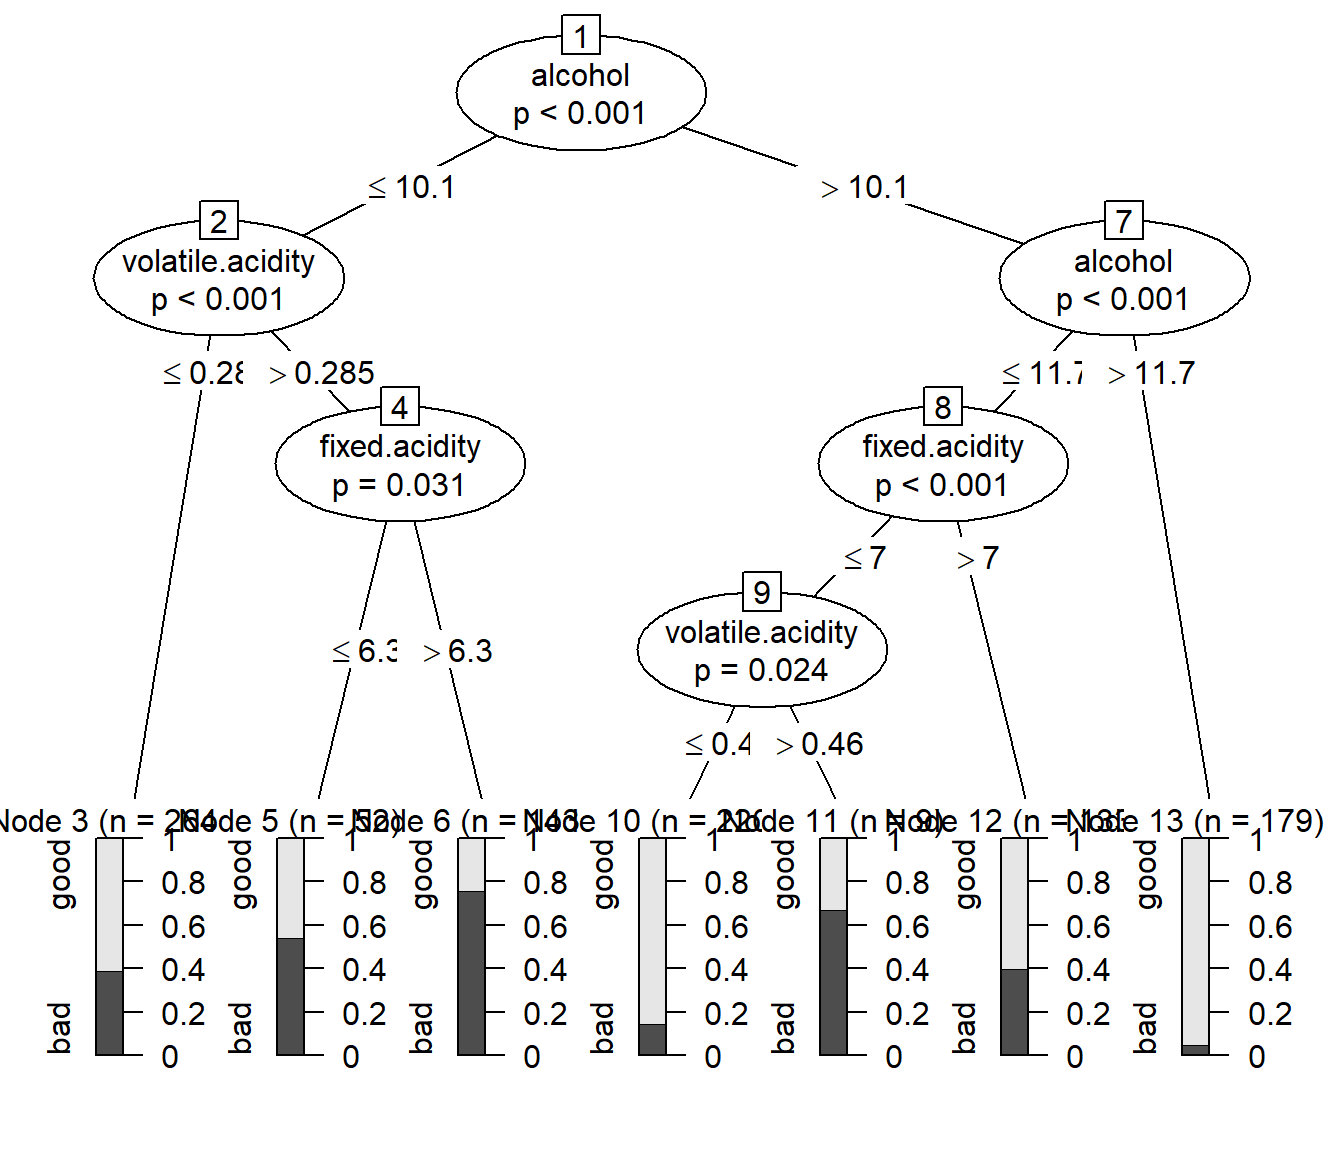
\includegraphics[width=0.8\linewidth]{02-arboles_files/figure-latex/unnamed-chunk-33-1} \end{center}

\chapter{Bagging y Boosting}\label{bagging-boosting}

Tanto el \emph{bagging} como el \emph{boosting} son procedimientos
generales para la reducción de la varianza de un método estadístico de
aprendizaje.

La idea básica consiste en combinar métodos de predicción sencillos
(débiles), es decir, con poca capacidad predictiva, para obtener un
método de predicción muy potente (y robusto). Estas ideas se pueden
aplicar tanto a problemas de regresión como de clasificación.

Son muy empleados con árboles de decisión: son predictores débiles y se
generan de forma rápida. Lo que se hace es construir muchos modelos
(crecer muchos árboles) que luego se combinan para producir predicciones
(promediando o por consenso).

\section{Bagging}\label{bagging}

En la década de 1990 empiezan a utilizarse los métodos \emph{ensemble}
(métodos combinados), esto es, métodos predictivos que se basan en
combinar las predicciones de cientos de modelos. Uno de los primeros
métodos combinados que se utilizó fue el \emph{bagging} (nombre que
viene de \emph{bootstrap aggregation}), propuesto en Breiman (1996). Es
un método general de reducción de la varianza que se basa en la
utilización del bootstrap junto con un modelo de regresión o de
clasificación, como puede ser un árbol de decisión.

La idea es muy sencilla. Si disponemos de muchas muestras de
entrenamiento, podemos utilizar cada una de ellas para entrenar un
modelo que después nos servirá para hacer una predicción. De este modo
tendremos tantas predicciones como modelos y por tanto tantas
predicciones como muestras de entrenamiento. El procedimiento
consistente en promediar todas las predicciones anteriores tiene dos
ventajas importantes: simplifica la solución y reduce mucho la varianza.

El problema es que en la práctica no suele disponerse más que de una
única muestra de entrenamiento. Aquí es donde entra en juego el
bootstrap, técnica especialmente útil para estimar varianzas, pero que
en esta aplicación se utiliza para reducir la varianza. Lo que se hace
es generar cientos o miles de muestras bootstrap a partir de la muestra
de entrenamiento, y después utilizar cada una de estas muestras
bootstrap como una muestra de entrenamiento (\emph{bootstrapped training
data set}).

Para un modelo que tenga intrínsecamente poca variabilidad, como puede
ser una regresión lineal, aplicar bagging puede ser poco interesante, ya
que hay poco márgen para mejorar el rendimiento. Por contra, es un
método muy importante para los árboles de decisión, porque un árbol con
mucha profundidad (sin podar) tiene mucha variabilidad: si modificamos
ligeramente los datos de entrenamiento es muy posible que se obtenga un
nuevo árbol completamente distinto al anterior; y esto se ve como un
inconveniente. Por esa razón, en este contexto encaja perfectamente la
metodología bagging.

Así, para árboles de regresión se hacen crecer muchos árboles (sin poda)
y se calcula la media de las predicciones. En el caso de los árboles de
clasificación lo más sencillo es sustituir la media por la moda y
utilizar el criterio del voto mayoritario: cada modelo tiene el mismo
peso y por tanto cada modelo aporta un voto. Además, la proporción de
votos de cada categoría es una estimación de su probabilidad.

Una ventaja adicional del bagging es que permite estimar el error de la
predicción de forma directa, sin necesidad de utilizar una muestra de
test o de aplicar validación cruzada u, otra vez, remuestreo, y se
obtiene un resultado similar al que obtendríamos con estos métodos. Es
bien sabido que una muestra bootstrap va a contener muchas observaciones
repetidas y que, en promedio, sólo utiliza aproximadamente dos tercios
de los datos (para ser más precisos,
\(1 - (1 - 1/n)^n \approx 1 - e^{-1} = 0.6321\) al aumentar el tamaño
del conjunto de datos de entrenamiento). Un dato que no es utilizado
para construir un árbol se denomina un dato \emph{out-of-bag} (OOB). De
este modo, para cada observación se pueden utilizar los árboles para los
que esa observación es \emph{out-of-bag} (aproximadamente una tercera
parte de los árboles construidos) para generar una única predicción para
ella. Repitiendo el proceso para todas las observaciones se obtiene una
medida del error.

Una decisión que hay que tomar es cuántas muestras bootstrap se toman (o
lo que es lo mismo, cuántos árboles se construyen). Realmente se trata
de una aproximación Monte Carlo, por lo que típicamente se estudia
gráficamente la convergencia del error OOB al aumentar el número de
árboles (para más detalles ver p.e. Fernández-Casal y Cao, 2020,
\href{https://rubenfcasal.github.io/simbook/convergencia.html}{Sección
4.1}). Si aparentemente hay convergencia con unos pocos cientos de
árboles, no va a variar mucho el nivel de error al aumentar el número.
Por tanto aumentar mucho el número de árboles no mejora las
predicciones, aunque tampoco aumenta el riesgo de sobreajuste. Los
costes computacionales aumentan con el número de árboles, pero la
construcción y evaluación del modelo son fácilmente paralelizables
(aunque pueden llegar a requerir mucha memoria si el conjunto de datos
es muy grande). Por otra parte si el número de árboles es demasiado
pequeño puede que se obtengan pocas (o incluso ninguna) predicciones OOB
para alguna de las observaciones de la muestra de entrenamiento.

Una ventaja que ya sabemos que tienen los árboles de decisión es su
fácil interpretabilidad. En un árbol resulta evidente cuales son los
predictores más influyentes. Al utilizar bagging se mejora (mucho) la
predicción, pero se pierde la interpretabilidad. Aún así, hay formas de
calcular la importancia de los predictores. Por ejemplo, si fijamos un
predictor y una medida del error podemos, para cada uno de los árboles,
medir la reducción del error que se consigue cada vez que hay un corte
que utilice ese predictor particular. Promediando sobre todos los
árboles bagging se obtiene una medida global de la importancia: un valor
alto en la reducción del error sugiere que el predictor es importante.

En resumen:

\begin{itemize}
\item
  Se remuestrea repetidamente el conjunto de datos de entrenamiento.
\item
  Con cada conjunto de datos se entrena un modelo.
\item
  Las predicciones se obtienen promediando las predicciones de los
  modelos (la decisión mayoritaria en el caso de clasificación).
\item
  Se puede estimar la precisión de las predicciones con el error OOB
  (out-of-bag).
\end{itemize}

\section{Bosques aleatorios}\label{bosques-aleatorios}

Los bosques aleatorios (\emph{random forest}) son una variante de
bagging específicamente diseñados para trabajar con árboles de decisión.
Las muestras bootstrap que se generan al hacer bagging introducen un
elemento de aleatoriedad que en la práctica provoca que todos los
árboles sean distintos, pero en ocasiones no son lo
\emph{suficientemente} distintos. Es decir, suele ocurrir que los
árboles tengan estructuras muy similares, especialmente en la parte
alta, aunque después se vayan diferenciando según se desciende por
ellos. Esta característica se conoce como correlación entre árboles y se
da cuando el árbol es un modelo adecuado para describir la relación ente
los predictores y la respuesta, y también cuándo uno de los predictores
es muy fuerte, es decir, es especialmente relevante, con lo cual casi
siempre va a estar en el primer corte. Esta correlación entre árboles se
va a traducir en una correlación entre sus predicciones (más
formalmente, entre los predictores).

Promediar variables altamente correladas produce una reducción de la
varianza mucho menor que si promediamos variables incorreladas. La
solución pasa por añadir aleatoriedad al proceso de construcción de los
árboles, para que estos dejen de estar correlados. Hubo varios intentos,
entre los que destaca Dietterich (2000) al proponer la idea de
introducir aleatorieadad en la selección de las variables de cada corte.
Breiman (2001) propuso un algoritmo unificado al que llamó bosques
aleatorios. En la construcción de cada uno de los árboles que finalmente
constituirán el bosque, se van haciendo cortes binarios, y para cada
corte hay que seleccionar una variable predictora. La modificación
introducida fue que antes de hacer cada uno de los cortes, de todas las
\(p\) variables predictoras, se seleccionan al azar \(m < p\)
predictores que van a ser los candidatos para el corte.

El hiperparámetro de los bosques aleatorios es \(m\), y se puede
seleccionar mediante las técnicas habituales. Como puntos de partida
razonables se pueden considerar \(m = \sqrt{p}\) (para problemas de
clasificación) y \(m = p/3\) (para problemas de regresión). El número de
árboles que van a constituir el bosque también puede tratarse como un
hiperparámetro, aunque es más frecuente tratarlo como un problema de
convergencia. En general, van a hacer falta más árboles que en bagging.

Los bosques aleatorios son computacionalmente más eficientes que bagging
porque, aunque como acabamos de decir requieren más árboles, la
construcción de cada árbol es mucho más rápida al evaluarse sólo unos
pocos predictores en cada corte.

Este método también puede ser empleado para aprendizaje no supervisado,
por ejemplo se puede construir una matriz de proximidad entre
observaciones a partir de la proporción de veces que están en un mismo
nodo terminal (para más detalles ver
\href{https://www.r-project.org/doc/Rnews/Rnews_2002-3.pdf}{Liaw y
Wiener, 2002}).

En resumen:

\begin{itemize}
\item
  Los bosques aleatorios son una modificación del bagging para el caso
  de árboles de decisión.
\item
  También se introduce aleatoriedad en las variables, no sólo en las
  observaciones.
\item
  Para evitar dependencias, los posibles predictores se seleccionan al
  azar en cada nodo (e.g. \(m=\sqrt{p}\)).
\item
  Se utilizan árboles sin podar.
\item
  Estos métodos dificultan la interpretación.
\item
  Se puede medir la importancia de las variables (índices de
  importancia).

  \begin{itemize}
  \item
    Por ejemplo, para cada árbol se suman las reducciones en el índice
    de Gini correspondientes a las divisiones de un predictor y
    posteriormente se promedian los valores de todos los árboles.
  \item
    Alternativamente (Breiman, 2001) se puede medir el incremento en el
    error de predicción OOB al permutar aleatoriamente los valores de la
    variable explicativa en la muestra OOB (manteniendo el resto sin
    cambios).
  \end{itemize}
\end{itemize}

\section{Bagging y bosques aleatorios en
R}\label{bagging-y-bosques-aleatorios-en-r}

Estos algoritmos son de los más populares en AE y están implementados en
numerosos paquetes de R, aunque la referencia es el paquete
\href{https://CRAN.R-project.org/package=randomForest}{\texttt{randomForest}}
(que emplea el código Fortran desarrollado por Leo Breiman y Adele
Cutler). La función principal es \texttt{randomForest()} y se suele
emplear de la forma:

\texttt{randomForest(formula,\ data,\ ntree,\ mtry,\ nodesize,\ ...)}

\begin{itemize}
\item
  \texttt{formula} y \texttt{data} (opcional): permiten especificar la
  respuesta y las variables predictoras de la forma habitual
  (típicamente \texttt{respuesta\ \textasciitilde{}\ .}), aunque si el
  conjunto de datos es muy grande puede ser preferible emplear una
  matriz o un data.frame para establecer los predictores y un vector
  para la respuesta (sustituyendo estos argumentos por \texttt{x} e
  \texttt{y}).
\item
  \texttt{ntree}: número de árboles que se crecerán; por defecto 500.
\item
  \texttt{mtry}: número de predictores seleccionados al azar en cada
  división; por defecto \texttt{max(floor(p/3),\ 1)} en el caso de
  regresión y \texttt{floor(sqrt(p))} en clasificación, siendo
  \texttt{p\ =\ ncol(x)\ =\ ncol(data)\ -\ 1} el número de predictores.
\item
  \texttt{nodesize}: número mínimo de observaciones en un nodo terminal;
  por defecto 1 en clasificación y 5 en regresión (puede ser
  recomendable incrementarlo si el conjunto de datos es muy grande, para
  evitar posibles problemas de sobreajuste, dismunir el tiempo de
  computación y los requerimientos de memoria; también podría ser
  considerado como un hiperparámetro).
\end{itemize}

Otros argumentos que pueden ser de interés\footnote{Si se quiere
  minimizar el uso de memoria, por ejemplo mientras se seleccionan
  hiperparámetros, se puede establecer \texttt{keep.forest=FALSE}.} son:

\begin{itemize}
\item
  \texttt{maxnodes}: número máximo de nodos terminales (como alternativa
  para la establecer la complejidad).
\item
  \texttt{importance\ =\ TRUE}: permite obtener medidas adicionales de
  importancia.
\item
  \texttt{proximity\ =\ TRUE}: permite obtener una matriz de
  proximidades (componente \texttt{\$proximity}) entre las observaciones
  (frecuencia con la que los pares de observaciones están en el mismo
  nodo terminal).
\item
  \texttt{na.action\ =\ na.fail}: por defecto no admite datos faltantes
  con la interfaz de fórmulas. Si los hubiese, se podrían imputar
  estableciento \texttt{na.action\ =\ na.roughfix} (empleando medias o
  modas) o llamando previamente a \texttt{rfImpute()} (que emplea
  proximidades obtenidas con un bosque aleatorio).
\end{itemize}

Más detalles en la ayuda de esta función o en
\href{https://www.r-project.org/doc/Rnews/Rnews_2002-3.pdf}{Liaw y
Wiener (2002)}.

Entre las numerosas alternativas, además de las implementadas en
paquetes que integran colecciones de métodos como \texttt{h2o} o
\texttt{RWeka}, una de las más utilizadas son los bosques aleatorios con
\emph{conditional inference trees}, implementada en la función
\texttt{cforest()} del paquete
\href{https://CRAN.R-project.org/package=party}{\texttt{party}}.

\subsection{Ejemplo: Clasificación con
bagging}\label{ejemplo-clasificaciuxf3n-con-bagging}

Como ejemplo consideraremos el conjunto de datos de calidad de vino
empleado en la Sección \ref{class-rpart} (para hacer comparaciones con
el ajuste de un único árbol).

\begin{Shaded}
\begin{Highlighting}[]
\KeywordTok{load}\NormalTok{(}\StringTok{"data/winetaste.RData"}\NormalTok{)}
\KeywordTok{set.seed}\NormalTok{(}\DecValTok{1}\NormalTok{)}
\NormalTok{df <-}\StringTok{ }\NormalTok{winetaste}
\NormalTok{nobs <-}\StringTok{ }\KeywordTok{nrow}\NormalTok{(df)}
\NormalTok{itrain <-}\StringTok{ }\KeywordTok{sample}\NormalTok{(nobs, }\FloatTok{0.8} \OperatorTok{*}\StringTok{ }\NormalTok{nobs)}
\NormalTok{train <-}\StringTok{ }\NormalTok{df[itrain, ]}
\NormalTok{test <-}\StringTok{ }\NormalTok{df[}\OperatorTok{-}\NormalTok{itrain, ]}
\end{Highlighting}
\end{Shaded}

Al ser bagging con árboles un caso particular de bosques aleatorios
cuando \(m = p\), también podemos emplear \texttt{randomForest}:

\begin{Shaded}
\begin{Highlighting}[]
\KeywordTok{library}\NormalTok{(randomForest)}
\KeywordTok{set.seed}\NormalTok{(}\DecValTok{4}\NormalTok{) }\CommentTok{# NOTA: Fijamos esta semilla para ilustrar dependencia}
\NormalTok{bagtrees <-}\StringTok{ }\KeywordTok{randomForest}\NormalTok{(taste }\OperatorTok{~}\StringTok{ }\NormalTok{., }\DataTypeTok{data =}\NormalTok{ train, }\DataTypeTok{mtry =} \KeywordTok{ncol}\NormalTok{(train) }\OperatorTok{-}\StringTok{ }\DecValTok{1}\NormalTok{)}
\NormalTok{bagtrees}
\end{Highlighting}
\end{Shaded}

\begin{verbatim}
## 
## Call:
##  randomForest(formula = taste ~ ., data = train, mtry = ncol(train) -      1) 
##                Type of random forest: classification
##                      Number of trees: 500
## No. of variables tried at each split: 11
## 
##         OOB estimate of  error rate: 23.5%
## Confusion matrix:
##      good bad class.error
## good  565  97   0.1465257
## bad   138 200   0.4082840
\end{verbatim}

Con el método \texttt{plot()} podemos examinar la convergencia del error
en la muestra OOB (simplemente emplea \texttt{matplot()} para
representar la componente \texttt{\$err.rate}):

\begin{Shaded}
\begin{Highlighting}[]
\KeywordTok{plot}\NormalTok{(bagtrees, }\DataTypeTok{main =} \StringTok{"Tasas de error"}\NormalTok{)}
\KeywordTok{legend}\NormalTok{(}\StringTok{"topright"}\NormalTok{, }\KeywordTok{colnames}\NormalTok{(bagtrees}\OperatorTok{$}\NormalTok{err.rate), }\DataTypeTok{lty =} \DecValTok{1}\OperatorTok{:}\DecValTok{5}\NormalTok{, }\DataTypeTok{col =} \DecValTok{1}\OperatorTok{:}\DecValTok{6}\NormalTok{)}
\end{Highlighting}
\end{Shaded}

\begin{center}\includegraphics[width=0.8\linewidth]{03-bagging_boosting_files/figure-latex/unnamed-chunk-4-1} \end{center}

Como vemos que los errores se estabilizan podríamos pensar que
aparentemente hay convergencia (aunque situaciones de alta dependencia
entre los áboles dificultarían su interpretación).

Con la función \texttt{getTree()} podemos extraer los árboles
individuales. Por ejemplo el siguiente código permite extraer la
variable seleccionada para la primera división:

\begin{Shaded}
\begin{Highlighting}[]
\CommentTok{# View(getTree(bagtrees, 1, labelVar=TRUE))}
\NormalTok{split_var_}\DecValTok{1}\NormalTok{ <-}\StringTok{ }\KeywordTok{sapply}\NormalTok{(}\KeywordTok{seq_len}\NormalTok{(bagtrees}\OperatorTok{$}\NormalTok{ntree),}
                      \ControlFlowTok{function}\NormalTok{(i) }\KeywordTok{getTree}\NormalTok{(bagtrees, i, }\DataTypeTok{labelVar=}\OtherTok{TRUE}\NormalTok{)[}\DecValTok{1}\NormalTok{, }\StringTok{"split var"}\NormalTok{])}
\end{Highlighting}
\end{Shaded}

En este caso concreto podemos observar que siempre es la misma, lo que
indicaría una alta dependencia entre los distintos árboles:

\begin{Shaded}
\begin{Highlighting}[]
\KeywordTok{table}\NormalTok{(split_var_}\DecValTok{1}\NormalTok{)}
\end{Highlighting}
\end{Shaded}

\begin{verbatim}
## split_var_1
##              alcohol            chlorides          citric.acid 
##                  500                    0                    0 
##              density        fixed.acidity  free.sulfur.dioxide 
##                    0                    0                    0 
##                   pH       residual.sugar            sulphates 
##                    0                    0                    0 
## total.sulfur.dioxide     volatile.acidity 
##                    0                    0
\end{verbatim}

Por último evaluamos la precisión en la muestra de test:

\begin{Shaded}
\begin{Highlighting}[]
\NormalTok{pred <-}\StringTok{ }\KeywordTok{predict}\NormalTok{(bagtrees, }\DataTypeTok{newdata =}\NormalTok{ test)}
\NormalTok{caret}\OperatorTok{::}\KeywordTok{confusionMatrix}\NormalTok{(pred, test}\OperatorTok{$}\NormalTok{taste)}
\end{Highlighting}
\end{Shaded}

\begin{verbatim}
## Confusion Matrix and Statistics
## 
##           Reference
## Prediction good bad
##       good  145  42
##       bad    21  42
##                                           
##                Accuracy : 0.748           
##                  95% CI : (0.6894, 0.8006)
##     No Information Rate : 0.664           
##     P-Value [Acc > NIR] : 0.002535        
##                                           
##                   Kappa : 0.3981          
##                                           
##  Mcnemar's Test P-Value : 0.011743        
##                                           
##             Sensitivity : 0.8735          
##             Specificity : 0.5000          
##          Pos Pred Value : 0.7754          
##          Neg Pred Value : 0.6667          
##              Prevalence : 0.6640          
##          Detection Rate : 0.5800          
##    Detection Prevalence : 0.7480          
##       Balanced Accuracy : 0.6867          
##                                           
##        'Positive' Class : good            
## 
\end{verbatim}

\subsection{Ejemplo: Clasificación con bosques
aleatorios}\label{ejemplo-clasificaciuxf3n-con-bosques-aleatorios}

Como ejemplo llamamos a la función \texttt{randomForest()} con las
opciones por defecto:

\begin{Shaded}
\begin{Highlighting}[]
\CommentTok{# load("data/winetaste.RData")}
\CommentTok{# set.seed(1)}
\CommentTok{# df <- winetaste}
\CommentTok{# nobs <- nrow(df)}
\CommentTok{# itrain <- sample(nobs, 0.8 * nobs)}
\CommentTok{# train <- df[itrain, ]}
\CommentTok{# test <- df[-itrain, ]}

\KeywordTok{set.seed}\NormalTok{(}\DecValTok{1}\NormalTok{)}
\NormalTok{rf <-}\StringTok{ }\KeywordTok{randomForest}\NormalTok{(taste }\OperatorTok{~}\StringTok{ }\NormalTok{., }\DataTypeTok{data =}\NormalTok{ train)}
\NormalTok{rf}
\end{Highlighting}
\end{Shaded}

\begin{verbatim}
## 
## Call:
##  randomForest(formula = taste ~ ., data = train) 
##                Type of random forest: classification
##                      Number of trees: 500
## No. of variables tried at each split: 3
## 
##         OOB estimate of  error rate: 22%
## Confusion matrix:
##      good bad class.error
## good  578  84   0.1268882
## bad   136 202   0.4023669
\end{verbatim}

En este caso también observamos que aparentemente hay convergencia y
tampoco sería necesario incrementar el número de árboles:

\begin{Shaded}
\begin{Highlighting}[]
\KeywordTok{plot}\NormalTok{(rf, }\DataTypeTok{main =} \StringTok{"Tasas de error"}\NormalTok{)}
\KeywordTok{legend}\NormalTok{(}\StringTok{"topright"}\NormalTok{, }\KeywordTok{colnames}\NormalTok{(rf}\OperatorTok{$}\NormalTok{err.rate), }\DataTypeTok{lty =} \DecValTok{1}\OperatorTok{:}\DecValTok{5}\NormalTok{, }\DataTypeTok{col =} \DecValTok{1}\OperatorTok{:}\DecValTok{6}\NormalTok{)}
\end{Highlighting}
\end{Shaded}

\begin{center}\includegraphics[width=0.8\linewidth]{03-bagging_boosting_files/figure-latex/unnamed-chunk-9-1} \end{center}

Podemos mostrar la importancia de las variables predictoras con la
función \texttt{importance()} o representarlas con
\texttt{varImpPlot()}:

\begin{Shaded}
\begin{Highlighting}[]
\KeywordTok{importance}\NormalTok{(rf)}
\end{Highlighting}
\end{Shaded}

\begin{verbatim}
##                      MeanDecreaseGini
## fixed.acidity                37.77155
## volatile.acidity             43.99769
## citric.acid                  41.50069
## residual.sugar               36.79932
## chlorides                    33.62100
## free.sulfur.dioxide          42.29122
## total.sulfur.dioxide         39.63738
## density                      45.38724
## pH                           32.31442
## sulphates                    30.32322
## alcohol                      63.89185
\end{verbatim}

\begin{Shaded}
\begin{Highlighting}[]
\KeywordTok{varImpPlot}\NormalTok{(rf)}
\end{Highlighting}
\end{Shaded}

\begin{center}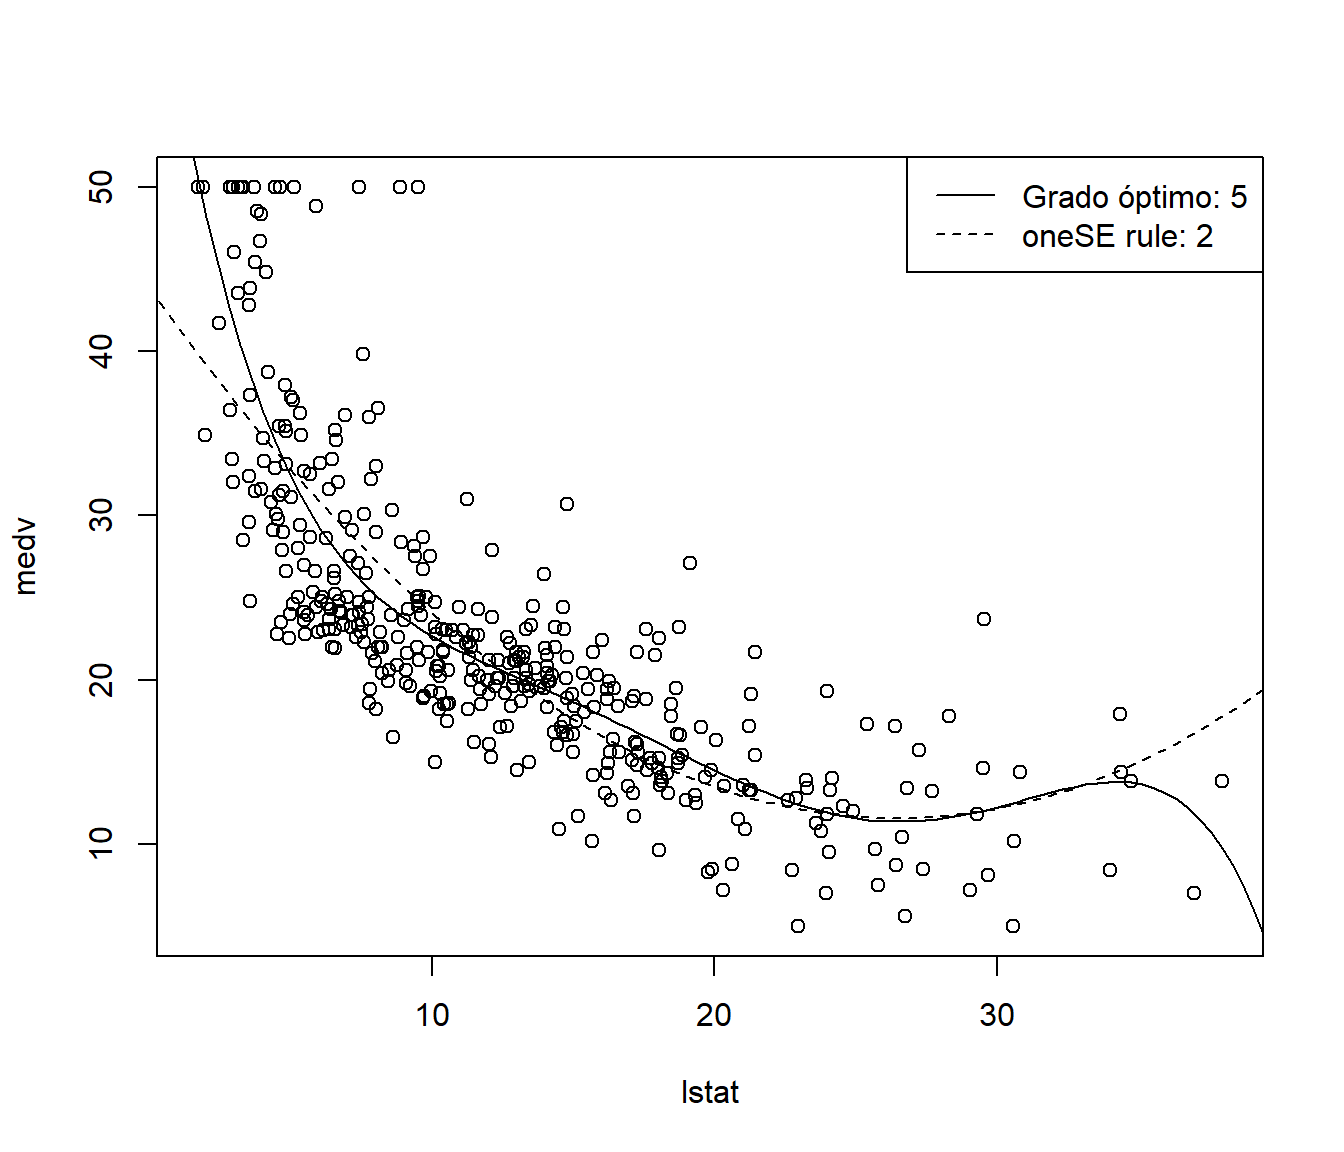
\includegraphics[width=0.8\linewidth]{03-bagging_boosting_files/figure-latex/unnamed-chunk-10-1} \end{center}

Si evaluamos la precisión en la muestra de test podemos observar un
ligero incremento en la precisión en comparación con el método anterior:

\begin{Shaded}
\begin{Highlighting}[]
\NormalTok{pred <-}\StringTok{ }\KeywordTok{predict}\NormalTok{(rf, }\DataTypeTok{newdata =}\NormalTok{ test)}
\NormalTok{caret}\OperatorTok{::}\KeywordTok{confusionMatrix}\NormalTok{(pred, test}\OperatorTok{$}\NormalTok{taste)}
\end{Highlighting}
\end{Shaded}

\begin{verbatim}
## Confusion Matrix and Statistics
## 
##           Reference
## Prediction good bad
##       good  153  43
##       bad    13  41
##                                           
##                Accuracy : 0.776           
##                  95% CI : (0.7192, 0.8261)
##     No Information Rate : 0.664           
##     P-Value [Acc > NIR] : 7.227e-05       
##                                           
##                   Kappa : 0.4494          
##                                           
##  Mcnemar's Test P-Value : 0.0001065       
##                                           
##             Sensitivity : 0.9217          
##             Specificity : 0.4881          
##          Pos Pred Value : 0.7806          
##          Neg Pred Value : 0.7593          
##              Prevalence : 0.6640          
##          Detection Rate : 0.6120          
##    Detection Prevalence : 0.7840          
##       Balanced Accuracy : 0.7049          
##                                           
##        'Positive' Class : good            
## 
\end{verbatim}

Debida a que en este caso la dependencia entre los árboles es menor:

\begin{Shaded}
\begin{Highlighting}[]
\NormalTok{split_var_}\DecValTok{1}\NormalTok{ <-}\StringTok{ }\KeywordTok{sapply}\NormalTok{(}\KeywordTok{seq_len}\NormalTok{(rf}\OperatorTok{$}\NormalTok{ntree),}
                      \ControlFlowTok{function}\NormalTok{(i) }\KeywordTok{getTree}\NormalTok{(rf, i, }\DataTypeTok{labelVar=}\OtherTok{TRUE}\NormalTok{)[}\DecValTok{1}\NormalTok{, }\StringTok{"split var"}\NormalTok{])}
\KeywordTok{table}\NormalTok{(split_var_}\DecValTok{1}\NormalTok{)}
\end{Highlighting}
\end{Shaded}

\begin{verbatim}
## split_var_1
##              alcohol            chlorides          citric.acid 
##                  150                   49                   38 
##              density        fixed.acidity  free.sulfur.dioxide 
##                  114                   23                   20 
##                   pH       residual.sugar            sulphates 
##                   11                    0                    5 
## total.sulfur.dioxide     volatile.acidity 
##                   49                   41
\end{verbatim}

\subsection{\texorpdfstring{Ejemplo: bosques aleatorios con
\texttt{caret}}{Ejemplo: bosques aleatorios con caret}}\label{ejemplo-bosques-aleatorios-con-caret}

En paquete \texttt{caret} hay varias implementaciones de bagging y
bosques aleatorios\footnote{Se puede hacer una búsqueda en la tabla del
  \href{https://topepo.github.io/caret/available-models.html}{Capítulo
  6: Available Models} del manual.}, incluyendo el algoritmo del paquete
\texttt{randomForest} considerando como hiperparámetro el número de
predictores seleccionados al azar en cada división \texttt{mtry}. Para
ajustar este modelo a una muestra de entrenamiento hay que establecer
\texttt{method\ =\ "rf"} en la llamada a \texttt{train()}.

\begin{Shaded}
\begin{Highlighting}[]
\KeywordTok{library}\NormalTok{(caret)}
\CommentTok{# str(getModelInfo("rf", regex = FALSE))}
\KeywordTok{modelLookup}\NormalTok{(}\StringTok{"rf"}\NormalTok{)}
\end{Highlighting}
\end{Shaded}

\begin{verbatim}
##   model parameter                         label forReg forClass probModel
## 1    rf      mtry #Randomly Selected Predictors   TRUE     TRUE      TRUE
\end{verbatim}

\begin{Shaded}
\begin{Highlighting}[]
\CommentTok{# load("data/winetaste.RData")}
\CommentTok{# set.seed(1)}
\CommentTok{# df <- winetaste}
\CommentTok{# nobs <- nrow(df)}
\CommentTok{# itrain <- sample(nobs, 0.8 * nobs)}
\CommentTok{# train <- df[itrain, ]}
\CommentTok{# test <- df[-itrain, ]}
\end{Highlighting}
\end{Shaded}

Con las opciones por defecto únicamente evalúa tres valores posibles del
hiperparámetro (se podría aumentar el número con \texttt{tuneLength} o
especificarlos con \texttt{tuneGrid}), pero aún así el tiempo de
computación puede ser alto (puede ser recomendable reducir el valor de
\texttt{nodesize} o paralelizar los cálculos; otras implementaciones
pueden ser más eficientes).

\begin{Shaded}
\begin{Highlighting}[]
\KeywordTok{set.seed}\NormalTok{(}\DecValTok{1}\NormalTok{)}
\NormalTok{rf.caret <-}\StringTok{ }\KeywordTok{train}\NormalTok{(taste }\OperatorTok{~}\StringTok{ }\NormalTok{., }\DataTypeTok{data =}\NormalTok{ train, }\DataTypeTok{method =} \StringTok{"rf"}\NormalTok{)}
\KeywordTok{plot}\NormalTok{(rf.caret)}
\end{Highlighting}
\end{Shaded}

\begin{center}\includegraphics[width=0.8\linewidth]{03-bagging_boosting_files/figure-latex/unnamed-chunk-14-1} \end{center}

Breiman (2001) sugiere emplear el valor por defecto, la mitad y el
doble:

\begin{Shaded}
\begin{Highlighting}[]
\NormalTok{mtry.class <-}\StringTok{ }\KeywordTok{sqrt}\NormalTok{(}\KeywordTok{ncol}\NormalTok{(train) }\OperatorTok{-}\StringTok{ }\DecValTok{1}\NormalTok{)}
\NormalTok{tuneGrid <-}\StringTok{ }\KeywordTok{data.frame}\NormalTok{(}\DataTypeTok{mtry =} \KeywordTok{floor}\NormalTok{(}\KeywordTok{c}\NormalTok{(mtry.class}\OperatorTok{/}\DecValTok{2}\NormalTok{, mtry.class, }\DecValTok{2}\OperatorTok{*}\NormalTok{mtry.class)))}
\KeywordTok{set.seed}\NormalTok{(}\DecValTok{1}\NormalTok{)}
\NormalTok{rf.caret <-}\StringTok{ }\KeywordTok{train}\NormalTok{(taste }\OperatorTok{~}\StringTok{ }\NormalTok{., }\DataTypeTok{data =}\NormalTok{ train,}
                  \DataTypeTok{method =} \StringTok{"rf"}\NormalTok{, }\DataTypeTok{tuneGrid =}\NormalTok{ tuneGrid)}
\KeywordTok{plot}\NormalTok{(rf.caret)}
\end{Highlighting}
\end{Shaded}

\begin{center}\includegraphics[width=0.8\linewidth]{03-bagging_boosting_files/figure-latex/unnamed-chunk-15-1} \end{center}

\section{Boosting}\label{boosting}

La metodología \emph{boosting} es una metodología general de aprendizaje
lento en la que se combinan muchos modelos obtenidos mediante un método
con poca capacidad predictiva para, \emph{impulsados}, dar lugar a un
mejor predictor. Los árboles de decisión pequeños (construidos con poca
profundidad) resultan perfectos para esta tarea, al ser realmente malos
predictores (\emph{weak learners}), fáciles de combinar y generarse de
forma muy rápida.

El boosting nació en el contexto de los problemas de clasificación y
tardó varios años en poderse extender a los problemas de regresión. Por
ese motivo vamos a empezar viendo el boosting en clasificación.

La idea del boosting la desarrollaron Valiant (1984) y Kearns y Valiant
(1989), pero encontrar una implementación efectiva fue una tarea difícil
que no se resolvió satisfactoriamente hasta que Freund y Schapire (1996)
presentaron el algoritmo \emph{AdaBoost}, que rápidamente se convirtió
en un éxito.

Veamos, de forma muy esquemática, en que consiste el algoritmo AdaBoost
para un problema de clasificación en el que sólo hay dos categorías y en
el que se utiliza como clasificador débil un árbol de decisión con pocos
nodos terminales, sólo marginalmente superior a un clasificador
aleatorio. En este caso resulta más cómodo recodificar la variable
indicadora \(Y\) como 1 si éxito y -1 si fracaso.

\begin{enumerate}
\def\labelenumi{\arabic{enumi}.}
\item
  Seleccionar \(B\), número de iteraciones.
\item
  Se les asigna el mismo peso a todas las observaciones de la muestra de
  entrenamiento (\(1/n\)).
\item
  Para \(b = 1, 2,\ldots, B\), repetir:

  \begin{enumerate}
  \def\labelenumii{\alph{enumii}.}
  \item
    Ajustar el árbol utilizando las observaciones ponderadas.
  \item
    Calcular la proporción de errores en la clasificación \(e_b\).
  \item
    Calcular \(s_b = \text{log}((1 - e_b)/e_b)\).
  \item
    Actualizar los pesos de las observaciones. Los pesos de las
    observaciones correctamente clasificadas no cambian; se les da más
    peso a las observaciones incorrectamente clasificadas, multiplicando
    su peso anterior por \((1 - e_b)/e_b\).
  \end{enumerate}
\item
  Dada una observación \(\mathbf{x}\), si denotamos por
  \(\hat y_b ( \mathbf{x} )\) su clasificación utilizando árbol
  \(b\)-ésimo, entonces
  \(\hat y( \mathbf{x} ) = signo \left( \sum_b s_b \hat y_b ( \mathbf{x} ) \right)\)
  (si la suma es positiva, se clasifica la observación como
  perteneciente a la clase +1, en caso contrario a la clase -1).
\end{enumerate}

Vemos que el algoritmo AdaBoost no combina árboles independientes (como
sería el caso de los bosques aleatorios, por ejemplo), sino que estos se
van generando en una secuencia en la que cada árbol depende del
anterior. Se utiliza siempre el mismo conjunto de datos (de
entrenamiento), pero a estos datos se les van poniendo unos pesos en
cada iteración que dependen de lo que ha ocurrido en la iteración
anterior: se les da más peso a las observaciones mal clasificadas para
que en sucesivas iteraciones se clasifiquen bien. Finalmente, la
combinación de los árboles se hace mediante una suma ponderada de las
\(B\) clasificaciones realizadas. Los pesos de esta suma son los valores
\(s_b\). Un árbol que clasifique de forma aleatoria \(e_b = 0.5\) va a
tener un peso \(s_b = 0\) y cuando mejor clasifique el árbol mayor será
su peso. Al estar utilizando clasificadores débiles (árboles pequeños)
es de esperar que los pesos sean en general próximos a cero.

El siguiente hito fue la aparición del método \emph{gradient boosting
machine} (Friedman, 2001), perteneciente a la familia de los métodos
iterativos de descenso de gradientes. Entre otras muchas ventajas, este
método permitió resolver no sólo problemas de clasificación sino también
de regresión; y permitió la conexión con lo que se estaba haciendo en
otros campos próximos como pueden ser los modelos aditivos o la
regresión logística. La idea es encontrar un modelo aditivo que minimice
una función de perdida utilizando predictores débiles (por ejemplo
árboles).

Si como función de pérdida se utiliza RSS, entonces la pérdida de
utilizar \(m(x)\) para predecir \(y\) en los datos de entrenamiento es
\[L(m) = \sum_{i=1}^n L(y_i, m(x_i)) = \sum_{i=1}^n (y_i - m(x_i))^2\].

Se desea minimizar \(L(m)\) con respecto a \(m\) mediante el método de
los gradientes, pero estos son precisamente los residuos: si
\(L(m)= \frac{1}{2} (y_i - m(x_i))^2\), entonces
\[- \frac{\partial L(y_i, m(x_i))} {\partial m(x_i)} = y_i - m(x_i) = r_i\]
Una ventaja de esta aproximación es que puede extenderse a otras
funciones de pérdida, por ejemplo si hay valores atípicos se puede
considerar como función de pérdida el error absoluto.

Veamos el algoritmo para un problema de regresión utilizando árboles de
decisión. Es un proceso iterativo en el que lo que se \emph{ataca} no
son los datos directamente, sino los residuos (gradientes) que van
quedando con los sucesivos ajustes, siguiendo una idea greedy (la
optimización se resuelve en cada iteración, no globalmente).

\begin{enumerate}
\def\labelenumi{\arabic{enumi}.}
\item
  Seleccionar el número de iteraciones \(B\), el parámetro de
  regularización \(\lambda\) y el número de cortes de cada árbol \(d\).
\item
  Establecer una predicción inicial constante y calcular los residuos de
  los datos \(i\) de la muestra de entrenamiento:
  \[\hat m (x) = 0, \ r_i = y_i\]
\item
  Para \(b = 1, 2,\ldots, B\), repetir:

  \begin{enumerate}
  \def\labelenumii{\alph{enumii}.}
  \item
    Ajustar un árbol de regresión \(\hat m^b\) con \(d\) cortes
    utilizando los residuos como respuesta: \((X, r)\).
  \item
    Calcular la versión regularizada del árbol: \[\lambda \hat m^b (x)\]
  \item
    Actualizar los residuos:
    \[r_i \leftarrow r_i - \lambda \hat m^b (x_i)\]
  \end{enumerate}
\item
  Calcular el modelo boosting:
  \[\hat m (x) = \sum_{b=1}^{B} \lambda \hat m^b (x)\]
\end{enumerate}

Comprobamos que este método depende de 3 hiperparámetros, \(B\), \(d\) y
\(\lambda\), susceptibles de ser seleccionados de forma \emph{óptima}:

\begin{itemize}
\item
  \(B\) es el número de árboles. Un valor muy grande podría llegar a
  provocar un sobreajuste (algo que no ocurre ni con bagging ni con
  bosques aleatorios, ya que estos son métodos en los que se construyen
  árboles independientes). En cada iteración, el objetivo es ajustar de
  forma óptima el gradiente (en nuestro caso, los residuos), pero este
  enfoque greedy no garantiza el óptimo global y puede dar lugar a
  sobreajustes.
\item
  Al ser necesario que el aprendizaje sea lento se utilizan árboles muy
  pequeños. Esto consigue que poco a poco se vayan cubriendo las zonas
  en las que es más difícil predecir bien. En muchas situaciones
  funciona bien utilizar \(d = 1\), es decir, con un único corte. En
  este caso en cada \(\hat m^b\) interviene una única variable, y por
  tanto \(\hat m\) es un ajuste de un modelo aditivo. Si \(d>1\) se
  puede interpretar como un parámetro que mide el órden de interacción
  entre las variables.
\item
  \(0 < \lambda < 1\), parámetro de regularización. Las primeras
  versiones del algorimo utilizaban un \(\lambda = 1\), pero no
  funcionaba bien del todo. Se mejoró mucho el rendimiento
  \emph{ralentizando} aún más el aprendizaje al incorporar al modelo el
  parámetro \(\lambda\), que se puede interpretar como una proporción de
  aprendizaje (la velocidad a la que aprende, \emph{learning rate}).
  Valores pequeños de \(\lambda\) evitan el problema del sobreajuste,
  siendo habitual utilizar \(\lambda = 0.01\) o \(\lambda = 0.001\).
  Como ya se ha dicho, lo ideal es seleccionar su valor utilizando, por
  ejemplo, validación cruzada. Por supuesto, cuanto más pequeño sea el
  valor de \(\lambda\), más lento va a ser el proceso de aprendizaje y
  serán necesarias más iteraciones, lo cual incrementa los tiempos de
  cómputo.
\end{itemize}

El propio Friedman propuso una mejora de su algoritmo, inspirado por la
técnica bagging de Breiman. Esta variante, conocida como
\emph{stochastic gradient boosting}, es a día de hoy una de las más
utilizadas. La única diferencia respecto al algoritmo anterior es en la
primera línea dentro del bucle: al hacer el ajuste de \((X, r)\), no se
considera toda la muestra de entrenamiento, sino que se selecciona al
azar un subconjunto. Esto incorpora un nuevo hiperparámetro a la
metodología, la fracción que se utiliza de los datos. Lo ideal es
seleccionar un valor por algún método automático (\emph{tunearlo}) tipo
validación cruzada; una selección manual típica es 0.5. Hay otras
variantes, como por ejemplo la selección aleatoria de predictores antes
de crecer cada árbol o antes de cada corte (ver por ejemplo la
documentación de
\texttt{{[}h2o::gbm{]}(http://docs.h2o.ai/h2o/latest-stable/h2o-docs/data-science/gbm.html)}).

Este sería un ejemplo de un método con muchos hiperparámetros y diseñar
una buena estrategia para ajustarlos (\emph{tunearlos}) puede resultar
mucho más complicado (puede haber problemas de mínimos locales,
problemas computacionales, etc.).

\emph{Stochastic gradient boosting} incorpora dos ventajas importantes:
reduce la varianza y reduce los tiempos de cómputo. En terminos de
rendimiento tanto el método \emph{stochastic gradient boosting} como
\emph{random forest} son muy competitivos, y por tanto son muy
utilizando en la práctica. Los bosques aleatorios tienen la ventaja de
que, al construir árboles de forma independiente, es paralelizable y eso
puede reducir los tiempos de cómputo.

Otro método reciente que está ganando popularidad es \emph{extreme
gradient boosting}, también conocido como \emph{XGBoost} (Chen y
Guestrin, 2016). Es un metodo más complejo que el anterior que, entre
otras modificaciones, utiliza una función de pérdida con una
penalización por complejidad y, para evitar el sobreajuste, regulariza
utilizando la hessiana de la función de pérdida (necesita calcular las
derivadas parciales de primer y de segundo orden), e incorpora
parámetros de regularización adicionales para evitar el sobreajuste.

Por último, la importancia de las variables se puede medir de forma
similar a lo que ya hemos visto en otros métodos: dentro de cada árbol
se sumas las reducciones del error que consigue cada predictor, y se
promedia entre todos los árboles utilizados.

En resumen:

\begin{itemize}
\item
  La idea es hacer un ``aprendizaje lento''.
\item
  Los arboles se crecen de forma secuencial, se trata de mejorar la
  clasificación anterior.
\item
  Se utilizan arboles pequeños.
\item
  A diferencia de bagging y bosques aleatorios puede haber problemas de
  sobreajuste (si el número de árboles es grande y la tasa de
  aprendizaje es alta).
\item
  Se puede pensar que se ponderan las observaciones iterativamente, se
  asigna más peso a las que resultaron más difíciles de clasificar.
\item
  El modelo final es un modelo aditivo (media ponderada de los árboles).
\end{itemize}

\section{Boosting en R}\label{boosting-en-r}

En preparación\ldots{}

ada, adabag, mboost, gbm, xgboost

\chapter*{Referencias}\label{referencias}
\addcontentsline{toc}{chapter}{Referencias}

\section*{Bibliografía básica}\label{bibliografuxeda-buxe1sica}
\addcontentsline{toc}{section}{Bibliografía básica}

James, G., Witten, D., Hastie, T. y Tibshirani, R. (2013).
\emph{\href{http://faculty.marshall.usc.edu/gareth-james/ISL}{An
Introduction to Statistical Learning: with Aplications in R}}. Springer.

Kuhn, M. y Johnson, K. (2013).
\emph{\href{http://appliedpredictivemodeling.com}{Applied predictive
modeling}}. Springer.

Williams, G. (2011). \emph{Data Mining with Rattle and R}. Springer.

\section*{Bibliografía
complementaria}\label{bibliografuxeda-complementaria}
\addcontentsline{toc}{section}{Bibliografía complementaria}

\subsection*{Libros}\label{libros}
\addcontentsline{toc}{subsection}{Libros}

Bellman, R.E. (1961). \emph{Adaptive Control Processes}, Princeton
University Press.

Burger, S.V. (2018). \emph{Introduction to machine learning with R:
Rigorous mathematical analysis}. O'Reilly.

Breiman, L., Friedman, J., Stone, C.J. y Olshen, R.A. (1984).
\emph{Classification and regression trees}. CRC press.

Efron, B. y Hastie, T. (2016).
\emph{\href{http://web.stanford.edu/~hastie/CASI/}{Computer age
statistical inference}}. Cambridge University Press.

Fernández-Casal, R. y Cao, R. (2020). \emph{Simulación Estadística}.
\url{https://rubenfcasal.github.io/simbook}.

Hastie, T., Tibshirani, R. y Friedman, J. (2009).
\emph{\href{https://web.stanford.edu/~hastie/ElemStatLearn}{The Elements
of Statistical Learning: Data Mining, Inference, and Prediction}}.
Springer.

Hastie, T., Tibshirani, R. y Wainwright, M. (2015). \emph{Statistical
learning with sparsity: the lasso and generalizations}. CRC press.

Irizarry, R.A. (2019).
\emph{\href{https://rafalab.github.io/dsbook}{Introduction to Data
Science: Data Analysis and Prediction Algorithms with R}}. CRC Press.

Molnar, C. (2020).
\href{https://christophm.github.io/interpretable-ml-book}{Interpretable
Machine Learning. A Guide for Making Black Box Models Explainable}.
Lulu.com.

Torgo, L. (2011). \emph{Data Mining with R: Learning with Case Studies}.
Chapman \& Hall/CRC Press.

\subsection*{Artículos}\label{artuxedculos}
\addcontentsline{toc}{subsection}{Artículos}

Agor, J. y Özaltın, O.Y. (2019). Feature selection for classification
models via bilevel optimization. \emph{Computers \& Operations
Research}, 106, 156-168.

Biecek, P. (2018).
\href{http://www.jmlr.org/papers/volume19/18-416/18-416.pdf}{DALEX:
explainers for complex predictive models in R}. \emph{The Journal of
Machine Learning Research}, 19(1), 3245-3249.

Breiman, L. (1996). Bagging predictors. \emph{Machine Learning}, 24(2),
123-140.

Breiman, L. (2001). Random Forests. \emph{Machine Learning}, 45(1),
5--32.

Breiman, L. (2001). Statistical Modeling: The Two Cultures (with
comments and a rejoinder by the author). \emph{Statistical Science}, 16,
199-231.

Dietterich, T.G. (2000). An Experimental Comparison of Three Methods for
Constructing Ensembles of Decision Trees: Bagging, Boosting, and
Randomization. \emph{Machine Learning}, 40(2), 139--158.

Dunson D.B. (2018). Statistics in the big data era: Failures of the
machine. \emph{Statistics and Probability Letters}, 136, 4-9.

Fisher, R.A. (1936). The use of multiple measurements in taxonomic
problems. \emph{Annals of Eugenics}, 7(2), 179-188.

Freund, Y. y Schapire, R. (1996). Experiments with a New Boosting
Algorithm. \emph{Machine Learning: Proceedings of the Thirteenth
International Conference}, 148--156.

Friedman, J.H. (2001). Greedy Function Approximation: A Gradient
Boosting Machine. \emph{Annals of Statistics}, 29, 1189--1232.

Friedman, J.H. y Popescu, B.E. (2008). Predictive learning via rule
ensembles. \emph{The Annals of Applied Statistics}, 2(3), 916-954.
Goldstein, A., Kapelner, A., Bleich, J. y Pitkin, E. (2015).
\href{https://doi.org/10.1080/10618600.2014.907095}{Peeking inside the
black box: Visualizing statistical learning with plots of individual
conditional expectation}. \emph{Journal of Computational and Graphical
Statistics}, 24(1), 44-65.

Greenwell, B.M. (2017).
\href{https://journal.r-project.org/archive/2017/RJ-2017-016/index.html}{pdp:
An R Package for Constructing Partial Dependence Plots}. \emph{The R
Journal}, 9(1), 421-436.

Kearns, M. y Valiant, L. (1989). Cryptographic Limitations on Learning
Boolean Formulae and Finite Automata. \emph{Proceedings of the
Twenty-First Annual ACM Symposium on Theory of Computing}.

Kuhn, M. (2008). Building predictive models in R using the caret
package. \emph{Journal of Statistical Software}, 28(5), 1-26.

Lauro, C. (1996). Computational statistics or statistical computing, is
that the question?, \emph{Computational Statistics \& Data Analysis}, 23
(1), 191-193.

Liaw, A. y Wiener, M. (2002).
\href{https://www.r-project.org/doc/Rnews/Rnews_2002-3.pdf}{Classification
and regression by randomForest}. \emph{R News}, 2(3), 18-22.

Loh, W.Y. (2002). Regression tress with unbiased variable selection and
interaction detection. \emph{Statistica Sinica}, 361-386.

Shannon C (1948). A Mathematical Theory of Communication. \emph{The Bell
System Technical Journal}, 27, 379--423.

Strumbelj, E. y Kononenko, I. (2010). An efficient explanation of
individual classifications using game theory. \emph{Journal of Machine
Learning Research}, 11, 1-18.

Valiant, L. (1984). A Theory of the Learnable. \emph{Communications of
the ACM}, 27, 1134--1142.

\bibliography{book.bib,packages.bib}

\end{document}
